\documentclass[10pt,twocolumn,letterpaper]{article}
\usepackage[T1]{fontenc}
\usepackage[utf 8]{inputenc}
\usepackage{amsmath,amssymb,mathtools,bm}
\usepackage{mathptmx,mathrsfs,iftex}
\renewcommand{\ttdefault}{pcr}
\usepackage[margin=0.68in,columnsep=0.26in,headheight=14pt,headsep=0.15in,footskip=0.28in]{geometry}
\usepackage{graphicx,booktabs,array,tabularx,longtable}
\usepackage{microtype,fancyhdr,caption,titlesec,enumitem,balance}
\usepackage[hidelinks,bookmarksnumbered=true,hypertexnames=false,pdftitle={Clocks, signals, and calibrated observation},pdfauthor={Sean Brady; OpenAI ChatGPT and Codex},pdfsubject={Chapter IV combined development; source clocks, propagation, amplitude distances and finite-window inference}]{hyperref}
\usepackage{xurl}
\setlength{\parindent}{1em}
\setlength{\parskip}{0.10em}
\setlength{\emergencystretch}{1.6em}
\setlength{\abovedisplayskip}{6pt plus 2pt minus 2pt}
\setlength{\belowdisplayskip}{6pt plus 2pt minus 2pt}
\captionsetup{font=small,labelfont=bf,justification=raggedright,singlelinecheck=false}
\titleformat{\section}{\large\bfseries\raggedright}{\thesection.}{0.45em}{}
\titleformat{\subsection}{\normalsize\bfseries\raggedright}{\thesubsection}{0.45em}{}
\titlespacing*{\section}{0pt}{11pt plus 2pt minus 2pt}{5pt}
\titlespacing*{\subsection}{0pt}{8pt plus 2pt minus 2pt}{3pt}
\pagestyle{fancy}\fancyhf{}
\fancyhead[L]{\footnotesize SAM Volume I | Chapter IV}
\fancyhead[R]{\footnotesize Brady \;|\; 16 October 2026}
\fancyfoot[C]{\footnotesize\thepage}
\renewcommand{\headrulewidth}{0.3pt}
\newcommand{\dd}{\mathrm{d}}
\newcommand{\ii}{\mathrm{i}}
\newcommand{\Tr}{\operatorname{Tr}}
\newcommand{\Span}{\operatorname{span}}
\ifPDFTeX
\pdfmapfile{+cm.map}
\pdfmapfile{+cmextra.map}
\pdfmapfile{+symbols.map}
\pdfmapfile{+psnfss.map}
\pdfmapfile{+utm.map}
\pdfmapfile{=ps 2pk 35.map}
\pdfmapfile{+rsfs.map}
\fi
\ifdefined\pdfgentounicode\pdfgentounicode=1\fi

\usepackage{braket,float}
\linespread{1.06}
\providecommand{\mathbbm}[1]{\mathbb{#1}}
\ifdefined\DeclareUnicodeCharacter
\DeclareUnicodeCharacter{03B8}{\ensuremath{\theta}}
\DeclareUnicodeCharacter{03C6}{\ensuremath{\varphi}}
\fi

\newcommand{\sgn}{\operatorname{sgn}}
\newcommand{\diag}{\operatorname{diag}}
\newcommand{\rank}{\operatorname{rank}}
\newcommand{\Var}{\operatorname{Var}}
\newcommand{\Cov}{\operatorname{Cov}}

\newcommand{\Kcal}{\mathcal K}
\newcommand{\se}{\mathrm{s}}
\renewcommand{\succeq}{\mathrel{\geq}}
\renewcommand{\succ}{\mathrel{>}}
\renewcommand{\hbar}{\mathchar'26\mkern-9mu h}
\renewcommand{\angle}{\mathord{\mathchar"025C}}


\begin{document}
\lefthyphenmin=2\righthyphenmin=3\raggedbottom
\twocolumn[{
\begin{center}
{\small SAM VOLUME I\par}\vspace{0.4em}
{\LARGE\bfseries Clocks, signals,\ and calibrated observation\par}\vspace{0.4em}
{\large Chapter IV \textbullet\ Finite preparation and switched joint composition development\par}\vspace{0.5em}
{\large Sean Brady\par}
{\small Originator and conceptual director\par}
{\small OpenAI ChatGPT and Codex \textbullet\ Research collaborators and co-authors\par}
{\small 16 October 2026\par}
\end{center}
\begin{minipage}{0.97\textwidth}
\noindent\textbf{Abstract.} A distant measurement composes a physical source history, emission, propagation, detection and calibration. The original interacting clock retains its full energy, preparation and transient. One globally positive spatial profile gives signed first and finite response enclosures for all six preparations under shared units. A sharper current bound certifies all six weak-field phase budgets and the total sign throughout a finite amplitude interval; a signed short-prefix result below is distinguished from the unresolved full-window isolated correction. The canonical local tensor coupling adds pair kernels, directional angular return and a switched vacuum-reference payment. A static canonical joint Hamiltonian, the original-shell limit and an analytic weighted normal frame now close static joint evolution and the free switched quantum propagator. All six static canonical source phases are certified at the original full-cycle time. Exact positive smoothing sharply bounds the compact carrier's radiation energy, with a signed source-work and near-storage identity. The actual gapless Euclidean continuum has a closed transform and positive finite quadrature surrogates with controlled errors. Noisy inference retains one simultaneous covariance event and a coarse-winding/fine-final measurement budget. The joint continuation derives a phase-bearing finite-mode signal from every original preparation, with an explicit passive channel, detector, finite-repeat and complete energy account. Exact real-time memory and two-time emission bounds compose with a finite local pointer protocol in the original or uniform-lapse law, with conditional phase error below 0.174 nanoradians. The current SAM\_land finite donor/control preparation now composes with that original/uniform local record protocol, including failures, unequal branch weights, phase and work. A complete tensor graph-ideal and causal common-form construction also closes existence of the actual switched canonical joint singular-source propagator. Quantitative nonuniform local-output transfer, measured apparatus calibration, global vacuum ramp work and cosmological amplitude dynamics remain explicit.
\end{minipage}\vspace{0.9em}
}]

\section*{Part A. The interacting clock and its spatial coupling}

\section{One observable, five physical operations}
The preceding chapters established an original Write source, its interacting phase clock and a spatial receiving account. Observation now asks how those objects become a measured number. A local clock history is followed by emission, propagation, reception and recording. Each operation contributes a defined transformation. Their composition is the subject of this chapter.~[1--3]

The source clock is retained throughout. Its complete Hamiltonian, preparation and nonzero current determine the actual phase; a bare two-level oscillator is not substituted when a signal leaves the source. A common lapse can change the clock's internal age, a route can delay its information, and an amplitude law can change an inferred distance. These are distinct operands in the same measurement.

The combined treatment brings together the former endpoint/GPS and photon-road drafts, and the finite-redshift analysis.~[11,18,19] The organizing question is what each measured quantity determines. The endpoint sections concern phase and accumulated age. The timing sections concern a map between emission and reception events. The distance sections concern amplitudes and channel calibration. A common source-native action can connect them; such a connection must be calculated rather than supplied by reusing the same word ``accumulation.''

\begin{table}[htbp]\centering\small
\caption{Notation and operational role. The three response symbols are deliberately distinct.}
\begin{tabularx}{\columnwidth}{@{}l>{\raggedright\arraybackslash}X@{}}\toprule
Symbol & Meaning\\\midrule
$a$ & dimensionless source lift, $2GM/(c^2r)$ in the isolated monopole comparison\\
$N$ & lapse multiplying the complete clock history\\
$n_{\rm opt}$ & coordinate optical index for a declared route law\\
$p$ & positive distance-response exponent\\
$\eta$ & internal age of the interacting clock in model units\\
$F$ & increasing emission--reception event map\\
$\Xi$ & GW/EM amplitude-distance ratio\\
$C_{\rm cal}$ & constant relative channel calibration in the distance sections\\\bottomrule
\end{tabularx}\end{table}

\section{The source lift and the receiving convention}


For a stationary isolated source, retain the source lift and potential
\[
 a(r)=\frac{2GM}{c^2r},\qquad \Phi(r)=-\frac{c^2}{2}a(r)=-\frac{GM}{r}.
\]
Here $a$ is the source-generated lift above the background, rather than the complete floor-plus-source account. The endpoint coupling used below is
\[
 N(a)=\sqrt{1-a},\qquad 0\leq a<1.
\]
It is a declared receiving law. The Poisson kernel alone does not select it. For two stationary endpoints, with identical calibration and matched internal age or stationary reference clocks,
\[
 \frac{\text{rate}_2}{\text{rate}_1}
 =\frac{N(a_2)}{N(a_1)}
 =\sqrt{\frac{1-a_2}{1-a_1}}.
\]
A higher endpoint has smaller $a$ and a larger rate. To first order the fractional increase is
\[
 \frac{\text{rate}_2}{\text{rate}_1}-1
 =\frac{a_1-a_2}{2}+O(a_1^2+a_2^2)
 =\frac{\Phi_2-\Phi_1}{c^2}+O(a^2).
\]
The half coefficient belongs to this endpoint map. Assigning it to a photon path would be a different receiving prescription.

The background needs an explicit convention even in a local experiment. If instead the raw coupling is $N_{\rm raw}(a)=\sqrt{1-A_0-a}$, normalizing its source-free value gives
\[
 \frac{N_{\rm raw}(a)}{N_{\rm raw}(0)}
 =\sqrt{1-\frac{a}{1-A_0}}.
\]
A common $A_0$ therefore does not algebraically cancel from the nonlinear endpoint ratio. Its leading source coefficient is $1/[2(1-A_0)]$. With the $A_0=1/(12\pi)$ convention retained in Chapters II--III, this differs from $1/2$ by the factor $1.0272486\ldots$. A rescaled lift could absorb the factor only if its source equation, mass calibration and all receiving laws were changed consistently.~[2,3,9]

The present chapter uses the source-normalized coupling $N(a)$ stated above. This is a testable choice of the local response, not a claim that a nonlinear floor has disappeared by subtraction. At linear order a genuinely common additive potential reference cancels between endpoints; that simpler statement does not prove the nonlinear one.

% Inherited complete-Hamiltonian clock deductions, with source citations retained.


\section{The endpoint receiver is the interacting clock}
An endpoint clock must first be an observable with a preparation and an evolution. Chapter I supplies all three without replacing the source by an isolated ideal oscillator. Its sixteen-state source retains Swap $S$, the signed current operators $D,C$, and the even energy $E_{\mathrm{even}}$. On each original active lane $l$, with signed gap $d_l\ne 0$, the receiver is
\[
 Z_l=\frac{D+iC}{d_l},\qquad z_l=\langle Z_l\rangle,
 \qquad\theta_l=-\arg z_l.
\]
The phase is continuously unwrapped from $\theta_l(0)=0$. It is not the original common Write phase. Its rate $\nu_l=-\operatorname{Im}(\dot z_l/z_l)$ exists wherever the retained differentiable expectation is nonzero. The full Hamiltonian is
\[
 \mathcal H_0=H_s+H_f+H_{\mathrm{int}}+H_{\mathrm{ct}},
\]
with $H_s=\varepsilon(S+E_{\mathrm{even}})$, both field polarizations in $H_f$, $H_{\mathrm{int}}=-\varepsilon(D\phi_++C\phi_\times)$, and $H_{\mathrm{ct}}=\varepsilon^2\mu_{\rm ct}(D^2+C^2)$, $\mu_{\rm ct}=1/(4R_{\rm W})$. Here $R_{\rm W}$ is Chapter I's source coupling radius, distinct from the terrestrial radius used below. None of these terms is removed when the receiver is named a clock.~[1]

The actual preparation is the coherent superposition of the exact two hard-field branches, tensored with the common soft vacuum. It is an interacting source--field preparation, not a product of a bare source oscillator and its optimal classical field. Chapter III's energy comparisons distinguish those preparations explicitly.~[3]

For every original lane, Chapter I reports a certified interval on which
\[
 |z_{l,0}(s)|\ge m_l>0,\qquad
 0<\ell_l\le\nu_{l,0}(s)\le u_l.
\]
Here $s$ denotes the original dimensionless evolution parameter. The inherited window ends at $T_0=573049\pi$, one bare cycle, not one completed actual phase turn. For example, the outward lane 01 rate bounds are $3.490102929541\times 10^{-6}$ and $3.490102934505\times 10^{-6}$. These are source-reported certificates; this chapter uses them and does not claim a new execution.~[1,2]


\section{A changing uniform lapse gives an exact history}
A lapse that changes with time need not vary across the clock's own source and field. First consider that uniform case. Assume the original self-adjoint Hamiltonian $\mathcal H_0$ is unchanged, the preparation is fixed, and $N(s)>0$ and $f(s)$ are real, locally integrable functions. Declare the complete coupling
\[
 \mathcal H(s)=N(s)\mathcal H_0+f(s)I,
 \qquad\eta(s)=\int_0^sN(v)\,\dd v.
\]
The variable $\eta$ is internal age in model units. It must remain in the inherited clock window whenever that window's quantitative bounds are used.

\noindent\textbf{Exact history consequence.} The propagator and current expectation are
\[
\begin{aligned}
 U(s)&=\exp\left[-i\int_0^s f(v)\,\dd v\right]
              \exp[-i\eta(s)\mathcal H_0],\\
 z_l(s)&=z_{l,0}(\eta(s)),\qquad
 \theta_l(s)=\theta_{l,0}(\eta(s)),\\
 \nu_l(s)&=N(s)\nu_{l,0}(\eta(s))
 \quad\hbox{almost everywhere}.
\end{aligned}
\]
\textit{Proof.} Spectral calculus defines the displayed unitary for every initial vector. On the domain of $\mathcal H_0$, differentiation almost everywhere gives $iU'=\mathcal H(s)U$ and $U(0)=I$; extension by continuity gives the full unitary evolution. The scalar exponential cancels from expectations. Substitution in the same bounded current observable gives the first identity for $z_l$. Nonvanishing and the common initial branch give the phase identity, and the absolutely continuous chain rule gives its rate. No adiabatic approximation or commutation of distinct field components is used: all times multiply the same complete operator.

This extends Chapter III's constant-lapse control by a mathematical consequence of its hypothesis. It does not establish that a supplied gravitational field couples in this way. Nor does it introduce a new continuum energy-density construction. Positivity makes internal age increasing; the unitary formula itself needs only real integrable $N$.

Changing the lapse also has an energy account. For differentiable $N,f$ and a finite-energy preparation, $[\mathcal H(s),\mathcal H_0]=0$ keeps $E_0=\langle\mathcal H_0\rangle$ constant, while the supplied power is $\dot N E_0+\dot f$. Thus the signed work over a switch is $(N(T)-N(0))E_0+f(T)-f(0)$. A closed switch can have zero signed net work while still requiring apparatus, timing and reversible energy storage. The phase identity does not remove that account.~[2,3]


\section{Equal coordinate time and equal internal age}
Comparing two identically prepared copies requires stating which events are compared. For copies $A,B$ with cumulative ages $\eta_A,\eta_B$, the exact rate ratio at equal coordinate parameter is
\[
 \frac{\nu_A(s)}{\nu_B(s)}
 =\frac{N_A(s)}{N_B(s)}
  \frac{\nu_0(\eta_A(s))}{\nu_0(\eta_B(s))}.
\]
The second factor is present because the actual clock is slightly nonstationary. At matched internal age, choose $s_A,s_B$ with $\eta_A(s_A)=\eta_B(s_B)$. The baseline rates then cancel and the ratio is $N_A(s_A)/N_B(s_B)$. A strictly stationary reference provides the same cancellation without age matching.

For a differentiable static receiving law $N(a)$ with $N(0)=1$, differentiation at equal coordinate time gives, where $\nu_0'$ exists,
\[
 \left.\partial_a\nu(s;a)\right|_{a=0}
 =N'(0)\{\nu_0(s)+s\nu_0'(s)\}.
\]
The transient term must not be absorbed into an independently fitted lapse. If only the inherited continuously differentiable phase is available, use its accumulated comparison instead; that argument needs no second phase derivative.

These distinctions concern comparison protocol, not a correction to the exact time change. Identical instruments examined after different internal ages need not display identical instantaneous baseline frequencies. An endpoint application can use matched-age calibration, a stationary reference, or an explicit transient budget. Independent adjustment of each lane's bare parameter would cease to test a shared coupling.~[2,3]


\section{A correlated finite-phase comparison}
Accumulated phase retains the common underlying history and is therefore sharper than comparing two unrelated interval estimates. For equal coordinate duration $T$, suppose both ages lie in the same certified window and $\eta_A(T)\le\eta_B(T)$. Put $D_T=\eta_B(T)-\eta_A(T)$. The exact time change gives
\[
\begin{aligned}
 \theta_A(T)-\theta_B(T)
 &=-\int_{\eta_A(T)}^{\eta_B(T)}\nu_0(v)\,\dd v,\\
 -uD_T&\le\theta_A(T)-\theta_B(T)\le-\ell D_T.
\end{aligned}
\]
This follows immediately by integrating the same positive baseline rate. Even if the two instantaneous lapses cross, only their cumulative ages enter this final comparison. No sign is asserted when their ordering is unknown.

For a reference with $N_B=1$ and a declared source-only lapse $N_A(s)=\sqrt{1-a(s)}$, assume $0\le a(s)<1$. Since
\[
 \frac a 2\le 1-\sqrt{1-a}=\frac{a}{1+\sqrt{1-a}}
 \le\frac{a}{2-a},
\]
we obtain the finite, time-dependent bound
\[
 -u\int_0^T\frac{a(s)}{2-a(s)}\,\dd s
 \le\theta_A(T)-\theta_B(T)
 \le-\frac\ell 2\int_0^Ta(s)\,\dd s.
\]
A positive integral produces a strictly negative phase difference within the stated hypotheses and window. This conditional deduction is inherited from the endpoint draft; it is an exact comparison under the stated coupling.

For a constant lift, the frozen Earth example retained in Chapter III gives approximately $-4.37389$ nanoradians over one bare cycle across the six lanes. Its independent-enclosure criterion $a>1-(\ell/u)^2$ is a sufficient condition for separating independently bounded phases, not a threshold for the correlated sign. Two independent readouts with phase error at most $\delta$ require a predicted margin exceeding $2\delta$, together with the stated timing, preparation and branch-control budgets.~[2,3]


\section{Which energy changes the clock}
A complete Hamiltonian coupling is stronger than a replacement of the source parameter. Scaling only $\varepsilon$ to $N\varepsilon$ while holding the field fixed gives
\[
 \mathcal H_\varepsilon=NH_s+H_f+NH_{\mathrm{int}}+N^2H_{\mathrm{ct}},
\]
so its exact difference from $N\mathcal H_0$ is
\[
 \mathcal H_\varepsilon-N\mathcal H_0
 =(1-N)H_f+(N^2-N)H_{\mathrm{ct}}.
\]
The derivative of this residual at $a=0$ is $N'(0)(H_{\mathrm{ct}}-H_f)$. The counterterm is current-blind, while the free field can change the current through the interaction. The six unequal hard-branch second-order diagnostics retained in Chapters II and III demonstrate why replacing a bare frequency alone is not the full-scaling theorem. They are not bounds on the full finite-lift response.~[2,3]

Conversely, energy can change with no current response. Chapter III identifies the complete Hermitian source algebra invisible to every current history:
\[
 W=\bigoplus_{a<b}w_{ab}I_2\ \oplus\ W_{\mathrm{dark}}.
\]
It has real dimension 22; the four-dimensional dark block carries zero current. Time-dependent integrable members are also invisible. Requiring conservation reduces the source algebra to ten dimensions, represented by functions of $E_{\mathrm{even}}$. A scalar addition is only its simplest case. Thus clock reception does not determine the total energy or its gravitational reference.

The six prepared-lane first-order tests are weaker still: the all-states-in-each-lane first-order blind space has dimension 238, including off-block directions that can return a bright response at second order. A common measured slope can constrain a declared coupling family without reconstructing arbitrary microscopic couplings. These inherited visibility results explain why universality needs a physical law, not six separate frequency fits.~[3]


\section{A finite control criterion for the actual phase}
The exact uniform theorem has a useful stability test. Compare it, including any exactly current-blind source term, with a Hamiltonian containing an additional strongly measurable, self-adjoint residual $R(s)$ with locally integrable operator norm. Require the same initial state and well-defined propagators. Duhamel's identity and unitarity give
\[
 |z(T)-z_{\mathrm{ideal}}(T)|
 \le 2\|Z\|\int_0^T\|R(s)\|\,\dd s.
\]
Indeed the propagator difference has norm at most the integral, and the expectation difference has two terms, each bounded by $\|Z\|$ times that difference. On a preserved original lane, $\|Z\|=2$. Leakage outside it requires the full receiver norm or an additional projected-receiver leakage estimate.

Suppose $|z_{\mathrm{ideal}}|\ge m$ throughout the interval. Write $q=4\int_0^T\|R(s)\|\,\dd s$ for the lane-preserving case. If $q<m$, the error disks exclude zero at every prefix, and elementary tangent geometry gives
\[
 |\theta(T)-\theta_{\mathrm{ideal}}(T)|
 \le\arcsin(q/m).
\]
Continuity from the common initial state fixes the unwrapped branch. If the ideal negative phase shift against an unperturbed reference has magnitude at least $x$, with $0<x<1$, the strict sufficient sign condition is
\[
 q<m\sin x.
\]
If both copies have residual errors, their two angular budgets must be added.

Chapter III implements a rational constant-residual version using $m=M_{\mathrm{lower}}-E_{\mathrm{cycle}}$, $x=\ell aT_{\mathrm{lo}}/2$, and
\[
 \|R\|<\frac{m(x-x^3/6)}{4T_{\mathrm{hi}}}.
\]
Its reported six lane budgets are approximately $6.07387$--$6.07390\times 10^{-16}$ in model-energy operator norm. They support its stated lane-preserving $\|R\|\le a^2$ fixture at the frozen lift. They do not bound an arbitrary unbounded field perturbation or specify attainable laboratory accuracy.~[3]


\section{A closed nonuniform quantum receiving form}\label{sec:nonuniform}
The uniform theorem fixes a complete reference operator. A constructive next step is to receive the original continuum energy through a positive weight on its complete residual-energy map. This is a new Codex receiving construction. Its spatial incidence is explicit; it is not assigned to the original ledger or identified with a pointwise renormalized stress tensor.

On each original active lane the complete Hamiltonian has the form
\[
 \mathcal H_0=\varepsilon eI+\varepsilon S+K,\qquad
 q_K[\Psi]=\|T_g\Psi\|^2,
\]
where $g=\varepsilon d$ retains the signed lane gap. On the complete two-polarization Fock space, with $\sigma_+=\sigma_z$, $\sigma_\times=\sigma_y$,
\[
 (T_g\Psi)_\alpha(\omega)=\sqrt\omega\,a_\alpha(\omega)\Psi
 -\frac{g\,u(\omega)}{\sqrt\omega}\sigma_\alpha\Psi.
\]
The original finite smearing is $\mu=\int|u(\omega)|^2\dd\omega/\omega$, and the bounded shift has squared norm $c_g=2g^2\mu$. The weighted annihilation map $A$ is closed on $\mathcal Q=Q(H_f)$, with $\|A\Psi\|^2=q_f[\Psi]$. Since $T_g=A-F_g$ and $F_g$ is bounded, $T_g$ is closed on precisely the same domain. The elementary squared triangle inequalities give
\begin{equation}
 H_f\le2K+2c_gI,\qquad K\le2H_f+2c_gI
 \label{eq:equivalent-forms}
\end{equation}
as quadratic forms. Thus $1+K$ and $1+H_f$ have equivalent form norms, without a frequency or occupation cutoff. The original finite source matrices extend this construction to all sixteen source states, including the four dark dimensions.

Choose a bounded self-adjoint weight on the residual-energy output space. For the six phase certificates below it preserves the original source lane; a source-independent output weight is one sufficient choice. Require
\[
 0<N_-I\le W\le N_+I<\infty,
 \qquad q_{K,W}[\Phi,\Psi]=\langle T_g\Phi,WT_g\Psi\rangle.
\]
For fixed real source coefficient $N_s$, define
\[
 q_{\mathcal H[N_s,W]}[\Psi]
 =N_s\varepsilon e\|\Psi\|^2+N_s\varepsilon\langle\Psi,S\Psi\rangle
 +q_{K,W}[\Psi].
\]
Positive upper and lower bounds on $W$, Eq.~\eqref{eq:equivalent-forms}, and the bounded source term make this a closed semibounded form on $\mathcal Q$. The representation theorem supplies its self-adjoint Hamiltonian. When $W=NI$ and $N_s=N$, it is exactly $N\mathcal H_0$.

Expanding $\langle(A-F_g)\Phi,W(A-F_g)\Psi\rangle$ retains the weighted free term, both signed cross terms and the entire weighted counterterm $\langle F_g\Phi,WF_g\Psi\rangle$. The construction does not weight the free field and then discard the interaction or counterterm. A bounded nonconstant spatial profile may be received by a supplied isometry $J$ as $W_N=J^*M_NJ$. The choice of $J$ is part of the physical receiving interface. The integrated Hamiltonian alone does not reconstruct it, and a different local stress quantization can have additional vacuum, pair-creation, projector or boundary terms.

\section{An energy-form stability theorem for the actual clock}\label{sec:form-stability}
The free-field part is unbounded, so the bounded-residual criterion above is not automatically applicable. The common form domain supplies a different estimate. Compare a static $H_{\rm ref}=N\mathcal H_0$, $N>0$, with the same-source-coefficient form $H_{\rm act}=H_{\rm ref}+r$, where
\[
 |r[\Phi,\Psi]|\le\delta\sqrt{q_K[\Phi]q_K[\Psi]},\qquad
 0\le\delta<N.
\]
The weight family supplies this bound with $\delta=\|W-NI\|$. Start both evolutions from the identical normalized original preparation in $\mathcal Q$. Write their states as $\Psi(t),\chi(t)$ and their distance as $d_\Psi(t)=\|\Psi(t)-\chi(t)\|$. Common-form weak evolution gives
\begin{equation}
 d_\Psi(t)^2\le2\delta\int_0^t
 \sqrt{K_{\rm act}(s)K_{\rm ref}(s)}\,\dd s.
 \label{eq:weak-duhamel}
\end{equation}
\textit{Proof.} The trajectories are continuous in the common form norm and differentiable into its dual. Pair the two weak Schr\"odinger equations. Their reference terms cancel, giving $\dd\langle\Psi,\chi\rangle/\dd t=\ii r[\Psi,\chi]$. Since $d_\Psi^2=2-2\operatorname{Re}\langle\Psi,\chi\rangle$, integration and the form bound give Eq.~\eqref{eq:weak-duhamel}. Bounded spectral regularization in the two equivalent form norms justifies the product rule before passing to the weak limit. No finite operator norm is assigned to $H_f$ or $r$.

For bounded current $Z$, the two-state expectation expansion gives
\[
 |z_{\rm act}-z_{\rm ref}|\le2\|Z\|d_\Psi.
\]
On each preserved original lane $\|Z\|=2$. If the reference amplitude is at least $m>0$ and $4d_\Psi<m$ at every prefix, the same unwrapped phase branch exists and its error is at most $\arcsin(4d_\Psi/m)$. Leakage between lanes pays its full receiver norm and preparation account.

\section{A bootstrap uses the original correlated preparation}
Retain the six original complete-energy preparation ceilings and phase-error certificates. For $N\le1$ and times within the original window, they supply
\[
 K_{\rm ref}(t)\le\kappa
 =K_{{\rm prep},\mathrm{upper}}+\varepsilon_{\rm upper}E(T)_{\rm upper}.
\]
This is a ceiling on the complete positive $K$ in the actual correlated preparation. It retains the cancellation between free, signed interaction and counterterm contributions.

Energy conservation in the two static families gives
\[
 (N-\delta)K_{\rm act}(t)
 \le(N+\delta)\kappa+2N\varepsilon d_\Psi(t).
\]
For $\delta\le N/2$, it follows that $K_{\rm act}\le3\kappa+4\varepsilon d_\Psi$. Choose $d_*>0$ and put
\[
 K_*=3\kappa+4\varepsilon_{\rm upper}d_*,\qquad
 \delta_*=\min\left\{\frac{N_{\rm lower}}2,
 \frac{d_*^2}{4T_{\rm upper}\sqrt{\kappa K_*}}\right\}.
\]
For $\delta\le\delta_*$, the trajectory cannot first reach $d_*$. Before a first crossing its $K_{\rm act}$ is bounded by $K_*$; Eq.~\eqref{eq:weak-duhamel} at that crossing would give $d_*^2\le d_*^2/2$. Hence $d_\Psi(t)<d_*$ throughout the interval. This is a full-continuum state estimate on the chosen form family.

For the inherited frozen Earth lift, set $N=\sqrt{1-a}$, $x=\ell aT_{\rm lower}/2$, and $m=M_{\rm lower}-E(T)_{\rm upper}$. The actual source certificate has $0<x<1$. Choose
\[
 d_*=\frac{m(x-x^3/6)}8.
\]
Then $4d_*/m=(x-x^3/6)/2<\sin x$. The perturbed phase error is smaller than the ideal negative correlated shift, preserving its sign. Directed rational evaluation gives the six sufficient dimensionless weight budgets in Table~\ref{tab:form-budgets}.

The source-specific bootstrap yields the first budget column in Table~\ref{tab:form-budgets}. It controls the complete joint vector, which is stronger than needed for a phase readout. The following estimate uses the actual current algebra directly.

\section{A sharper current-specific continuum remainder}
The receiver supplies additional structure. On a retained lane, $Z=\sigma_z+\ii\sigma_y$ has norm two. The weighted annihilation part commutes with finite source matrices, and direct two-polarization Pauli algebra gives
\[
 \|[T_g,Z]\Psi\|\le2\sqrt{c_g}\|\Psi\|,\qquad
 \|[T_g,Z^*]\Psi\|\le2\sqrt{c_g}\|\Psi\|.
\]
Equivalently, the squared polarization commutator sum is exactly $8g^2\mu I=4c_gI$. Thus
\[
 \sqrt{K[Z\Xi]}\le2\sqrt{K[\Xi]}+2\sqrt{c_g}\|\Xi\|,
\]
and likewise for $Z^*$. Conservation of the complete reference Hamiltonian also gives $K[U_0(t)\Xi]\le K[\Xi]+2\varepsilon\|\Xi\|^2$.

For $\delta\le N/2$, the static actual energy supplies the global ceiling $k_A=3K_{{\rm prep},\rm upper}+4\varepsilon_{\rm upper}$. Applying the preceding evolution, current and evolution bounds to $B_T(s)=U_{\rm ref}(T-s)^*ZU_{\rm ref}(T-s)$ gives, for both $B_T$ and its adjoint on the normalized actual state,
\[
 K[B_T(s)\Psi(s)]\le k_B,
\]
\[
 k_B=\left[2\sqrt{k_A+2\varepsilon_{\rm upper}}+2\sqrt{c_{g,\rm upper}}\right]^2
       +8\varepsilon_{\rm upper}.
\]
Weak Heisenberg variation on the same common form domain then gives the exact identity
\[
\begin{aligned}
 z_{\rm act}(T)-z_{\rm ref}(T)=\ii\int_0^T\{&r[\Psi,B_T\Psi]\\
                    &-r[B_T^*\Psi,\Psi]\}\,\dd s,
\end{aligned}
\]
and hence the observable-specific bound
\[
 |z_{\rm act}(T)-z_{\rm ref}(T)|\le2\delta T\sqrt{k_Ak_B}.
\]
A sufficient phase-sign weight budget is therefore
\[
 \delta_{\rm linear}=\min\left\{\frac{N_{\rm lower}}2,
 \frac{m(x-x^3/6)}{4T_{\rm upper}\sqrt{k_Ak_B}}\right\}.
\]
Directed upper square roots give the second column of Table~\ref{tab:form-budgets}. Its current error is at most half the sine margin. Each estimate separately suffices; the larger of the two budgets can be used without combining their incompatible intermediate bounds.

\begin{table}[htbp]\centering\small
\caption{Sufficient dimensionless $\|W-NI\|$ budgets for the original six preparations. Rounded displays of exact outward operands; the two columns protect the full state and the actual current, respectively.}\label{tab:form-budgets}
\begin{tabular}{@{}lrr@{}}\toprule
Lane & State bootstrap & Current-specific\\\midrule
01 & $7.090598\!\times\!10^{-11}$ & $2.961257\!\times\!10^{-11}$\\
02 & $2.262032\!\times\!10^{-11}$ & $2.845597\!\times\!10^{-11}$\\
03 & $3.199329\!\times\!10^{-15}$ & $1.479745\!\times\!10^{-11}$\\
12 & $6.476681\!\times\!10^{-11}$ & $2.953179\!\times\!10^{-11}$\\
13 & $3.745512\!\times\!10^{-15}$ & $1.511229\!\times\!10^{-11}$\\
23 & $4.467330\!\times\!10^{-15}$ & $1.546471\!\times\!10^{-11}$\\
\bottomrule\end{tabular}\end{table}
Protecting the observed phase is substantially less costly than protecting the complete joint vector for lanes 03, 13 and 23. The smallest of the six available sufficient budgets is now approximately $1.4797\times10^{-11}$. The declared illustrative fixture $\delta=a^2$ fits all six. These are receiving-weight bounds in model coordinates, distinct from bounded-Hamiltonian energy norms and from achieved apparatus precision. A physical lapse profile must supply its actual incidence, support and weight error before receiving the certificate.

\section{First variation and the local spatial calculation}
For an affine static weight $W(\lambda)=NI+\lambda B$ with $\|B\|\le b$, the complete variation is the form
\[
 r_B[\Phi,\Psi]=\langle T_g\Phi,BT_g\Psi\rangle,\qquad
 |r_B[\Phi,\Psi]|\le b\sqrt{q_K[\Phi]q_K[\Psi]}.
\]
Let $U_0$ denote the reference evolution and $B_T(s)=U_0(T-s)^*ZU_0(T-s)$. The finite source current and these evolutions preserve $\mathcal Q$, so the weak first-order response is
\[
 z_1(T)=\ii\int_0^T\!\left\{
 r_B[\chi(s),B_T(s)\chi(s)]
 -r_B[B_T(s)^*\chi(s),\chi(s)]\right\}\dd s.
\]
For nonzero reference current, $\theta_1(T)=-\operatorname{Im}[z_1(T)/z_0(T)]$ on the same unwrapped branch. The common-domain justification and complete source-matrix certificate are retained in Appendix~\ref{app:form-proof}. Actual evaluation requires the supplied incidence $J/B$ and two-time joint-state matrix elements; an energy ceiling alone does not assign their value.

A separate source-shell coefficient change $\delta_s$ contributes bounded residual $|\delta_s|\varepsilon$ after keeping the even scalar payment in the energy ledger. It adds at most $|\delta_s|\varepsilon T$ to the state-distance budget. It shares the total phase allowance with the form error; preparation, timing, winding, reference and readout errors add their own terms. The remaining local calculation is to construct the actual stress/energy form and receive every term, including its vacuum and boundary conventions, into this common-domain comparison.

\section{An explicit spatial receiver for the original radial modes}
The positive residual-energy form admits a source-bound spatial incidence rather than an unspecified output weight. Retain the original regular quadrupole radial operator and normalized TT tensors. Its unitary spherical-Bessel transform is
\[
 (\mathcal H_2 f)(r)=\sqrt{\frac2\pi}\int_0^\infty k j_2(kr)f(k)\,\dd k.
\]
It maps $L^2(\dd k)$ unitarily to $L^2(r^2\dd r)$.
The identity $\int r^2j_2(kr)j_2(k'r)\dd r=\pi\delta(k-k')/(2k^2)$ fixes its normalization and retains the regular finite-energy extension at the origin. With the original angular isometry $\mathcal UQ=\sqrt{5/(8\pi)}\Lambda_nQ$, define
\[
 (Jf)(r,n)=\sum_{\alpha=+,\times}\mathcal Ue_\alpha(n)(\mathcal H_2 f_\alpha)(r).
\]
This $J$ is an isometry on the original two-polarization residual-energy output. A real bounded profile $0<N_-\le N(\mathbf x)\le N_+$ supplies $W_N=J^*NJ$ with the same positive bounds. The full closed form retains both cross terms and its entire counterterm.

This is a specified positive-frequency square-form spatial receiver. Identifying it with a pointwise canonical quantum stress tensor still requires the common local-action, vacuum, derivative-energy and boundary calculation. Its compressed domain does not silently add the full angular complement dynamics. For
\[
 A_{ab}(r)=\int N(r,n)\,\mathcal Ue_a:\mathcal Ue_b\,\dd\Omega,
\]
the spectral kernel is
\[
 W_{ab}(k,k')=\frac2\pi kk'\int_0^\infty
 r^2j_2(kr)j_2(k'r)A_{ab}(r)\dd r.
\]
A scalar spatial profile can therefore mix radial frequencies.

\section{Exact selection rules and the gradient complement}
The polarized TT contraction is
\[
 \begin{aligned}
 \Lambda Q:\Lambda Q'={}&\operatorname{tr}(QQ')
 -n^{\mathrm T}(QQ'+Q'Q)n\\
 &+\tfrac12(n^{\mathrm T}Qn)(n^{\mathrm T}Q'n).
 \end{aligned}
\]
Its spherical degrees are precisely among $L=0,2,4$. Thus every odd scalar harmonic and every scalar harmonic above degree four has zero compression. For the actual two driven tensors, write $C[h]_{ab}=\int h\,\mathcal Ue_a:\mathcal Ue_b\dd\Omega$. Exact integration gives
\[
\begin{gathered}
 C[1]=I,\quad C[x]=C[y]=C[z]=0,\\
 C[3z^2-1]=\tfrac47I,\quad C[P_4(z)]=\tfrac1{126}I,\\
 C[x^2-y^2]=C[2xy]=C[2xz]=C[2yz]=0,\\
 C[x^4-6x^2y^2+y^4]=\tfrac4{63}\begin{pmatrix}1&0\\0&-1\end{pmatrix},\\
 C[4xy(x^2-y^2)]=\tfrac4{63}\begin{pmatrix}0&1\\1&0\end{pmatrix}.
\end{gathered}
\]
The other degree-four components vanish. The real scalar angular image on the original pair is exactly the three-dimensional space of real symmetric matrices. On the entire five-STF image, the actual $L=0,2,4$ Gaunt map has rank fifteen. It realizes every small real symmetric five-coordinate weight with a bounded real scalar profile; positivity still constrains finite coefficients. The earlier imaginary antisymmetric polarization fixture belongs to a different realization class. Here $\{D,C\}=0$ and $D^2=C^2$ make the real weighted counterterm proportional to $D^2$, retaining all four original dark dimensions.

A vanishing compressed gradient does not remove its complement. With $P_5$ the full STF angular-image projector,
\[
 \begin{gathered}
 P_5zP_5=0,\\
 P_5z(I-P_5)zP_5\\
 =\operatorname{diag}(11/21,11/21,5/21,5/21,1/7).
 \end{gathered}
\]
The latter is positive and rank five, with rank two on the driven pair. A full angular evolution must retain this gradient leakage and its returning effect.

The global profile remains bounded and positive. Every polynomial Taylor expression below is restricted to the finite near ball; the actual bounded exterior remains in the far account. For a smooth source-centered profile, $N=N_0+g_ix_i+H_{ij}x_ix_j/2+\cdots$, its quadratic compression is
\[
 A(r)-N_0I=\frac{r^2}{42}(5\operatorname{tr}H+6H_{zz})I+\cdots.
\]
Cubic terms also cancel by parity. A fourth directional-derivative bound $M_4$ on $r\le L$ supplies
\[
 \delta_{\rm near}\le \frac{L^2}{42}|5\operatorname{tr}H+6H_{zz}|+\frac{M_4L^4}{24}.
\]
For $N=1-m/|\mathbf d+\mathbf x|+O(m^2/d^2)$, the leading term is $mr^2(1-3\cos^2\beta)/(7d^3)$. It vanishes at $\cos^2\beta=1/3$. Even a scalar polarization compression varies radially and need not become one common lapse for six different correlated preparations.

\section{An actual-state spatial tail and a finite profile criterion}
Let $K_{\rm in/out}[\Psi]=\|P_{\rm in/out}JT_g\Psi\|^2$ split the original complete positive form at radius $L$. The physical profile supplies
\[
 |r[\Phi,\Psi]|\le\delta_{\rm near}\sqrt{K_{\rm in}[\Phi]K_{\rm in}[\Psi]}
 +\delta_{\rm far}\sqrt{K_{\rm out}[\Phi]K_{\rm out}[\Psi]}.
\]
The exterior stays in this account. If $\|W-N_0I\|<N_0/2$, put $k_A=3K_{{\rm prep},\rm up}+4\varepsilon_{\rm up}$. A reference ceiling $K\le k_R$ and uniform tail ceiling $K_{\rm out}\le\eta_{\rm ref}(L)$ give
\[
 \|\Psi_{\rm act}(T)-\chi(T)\|^2
 \le2T\sqrt{k_A}\left[\delta_{\rm near}\sqrt{k_R}
                         +\delta_{\rm far}\sqrt{\eta_{\rm ref}(L)}\right].
\]
Four times the state-distance bound controls the actual current error. Comparing it to the retained nonzero reference amplitude supplies the same unwrapped arcsine phase criterion as before.

The tail can be bounded for the original exact preparation. The retained hard-branch pull-through identity gives, for $k\ge\lambda=64\Delta$,
\[
 a_\alpha(k)\Phi_j=g u_R(k)(H_h-E_j+k)^{-1}\sigma_\alpha\Phi_j,
 \quad H_h-E_j\ge-\Delta.
\]
For $H_j(k)=k(H_h-E_j+k)^{-1}$, spectral calculus gives $\|H_j\|\le64/63$ and $\|H_j'\|\le(1/4+64/3969)/k$. Applying the original Bessel transform to this Hilbert-space-valued function supplies an explicit conservative annihilation bound $\|A_\alpha(r)\|\le C_A(L)/r^2$ for $r\ge L\ge2R$. The retained derivation splits at $1/R$, integrates the low-frequency Bessel derivative envelope, and keeps all nine high-frequency sine/cosine products with phases $k(r\pm R)$.

The shift has the exact profile
\[
 F_\alpha(r)=\frac{g}{\pi\sqrt\kappa\,rR}
 Q_2\!\left(\frac{r^2+R^2}{2rR}\right)\sigma_\alpha\Phi,
\]
where its logarithmic shell singularity is square integrable. For $r\ge L$ it is bounded by $C_F(L)/r^4$, with
\[
 C_F(L)=\frac{16|g|R^2}{15\pi\sqrt\kappa(1-y_L^2)},\qquad
 y_L=\frac{2LR}{L^2+R^2}.
\]
Keeping both original branches, both polarizations and the common soft vacuum gives
\[
 K_{{\rm out},{\rm prep}}(L)\le
 \min\left\{K_{{\rm prep},\rm up},\frac{8C_A(L)^2}{L}
                              +\frac{4C_F(L)^2}{5L^5}\right\}.
\]
The original energy-norm Duhamel estimate $d_A^2\le8T^2g^2v_s(1+F_T+\lambda)$ then supplies
\[
 \eta_{\rm ref}(L)\le\min\{K_{{\rm prep},\rm up}+\varepsilon E(T),
               2K_{{\rm out},{\rm prep}}(L)+4(1+c_g)d_A^2\}.
\]
The comparison payment independent of $L$ is a bound feature, not an actual tail floor. At the illustrative radius $L=10^{15}R$ in model coordinates, the preparation-tail ceilings divided by the inherited $K_{\rm prep}$ ceilings are approximately $0.00275835$, $0.00166416$, $2.06463\times10^{-5}$, $0.00267798$, $2.23339\times10^{-5}$ and $2.43841\times10^{-5}$ in lane order 01,02,03,12,13,23. No SI ruler is assigned by these examples.

These receiving-form results supply an explicit incidence, realizable-weight classification, selection and complement certificates, and actual-state tail bounds. Appendix~\ref{app:tail-coefficient} displays the full standalone $C_A(L)$ coefficient. The Gaunt certificates do not evaluate the six time-dependent current-response integrals. The following six-lane continuation supplies one actual positive profile, a declared common dimensional ruler and evaluated response enclosures. It retains the isolated inhomogeneous two-time matrix elements as unresolved within those enclosures. These are kept separate from the local quantum stress identification.

\section{One physical profile for the six original preparations}
Fix a common model profile before evaluating any lane:
\[
 \begin{gathered}
 N_\alpha(\mathbf x)=1-\alpha V_{\mathbf e}(\mathbf x),\qquad
 V_{\mathbf e}=\frac{\sqrt2d}{\sqrt{d^2+|\mathbf x-d\mathbf e|^2}},\\
 \alpha=10^{-3},\quad d=10^{30}R,\quad |\mathbf e|=1,
 \quad N_\alpha(0)=n=0.999.
 \end{gathered}
\]
This softened Plummer profile is smooth and globally positive:
$1-\sqrt2\alpha\le N_\alpha<1$. Its positive Laplacian is consistent with
a finite positive-density body under a declared weak-potential Poisson
interpretation. That interpretation is an additional receiving assignment,
not a gravity law derived from the original source ledger.

The original radius, propagation speed, action chart and clock window
$T_0=573049\pi$ remain common to every preparation. For a fully specified
shared SI fixture, choose $R_{\rm phys}=10^{-19}\,\mathrm m$,
$c_{\rm phys}=299792458\,\mathrm{m\,s^{-1}}$, and explicitly assign
$I_u=\hbar$, with $h=6.62607015\,10^{-34}\,\mathrm{J\,s}$. Then
\[
 \ell_u=R_{\rm phys}/R,\qquad t_u=\ell_u/c_{\rm phys},
 \qquad E_u=\hbar/t_u.
\]
The resulting displays are $t_u\simeq2.03959635\,10^{-27}\,\mathrm s$,
$E_u\simeq5.17049276\,10^{-8}\,\mathrm J$,
$\epsilon E_u\simeq9.02277600\,10^{-14}\,\mathrm J$,
$T_0t_u\simeq3.67185784\,10^{-21}\,\mathrm s$, and
$d_{\rm phys}=10^{11}\,\mathrm m$. Outward intervals travel with the
source bundle. This is one declared calibration fixture shared by all six
lanes; the microscopic assignment of the original action and ruler remains
a separate source question.

At the source center,
\[
 \nabla N_\alpha=-\frac{\alpha\mathbf e}{2d},\qquad
 \operatorname{Hess}N_\alpha=\frac{\alpha}{2d^2}
       (I-\tfrac32\mathbf e\mathbf e^{\rm T}).
\]
The gradient has zero first compression but retains its full local angular
complement. For $\beta=\angle(\mathbf e,\mathbf e_z)$ the quadratic
compression is
\[
 A(r)-nI=\frac{\alpha r^2}{56d^2}
       (9-6\cos^2\beta)I+O(r^4/d^4).
\]
Parallel, transverse and $\cos^2\beta=1/3$ controls have coefficients
$3/56,9/56,7/56$ times $\alpha r^2/d^2$. The last angle cancels the
trace-free tidal part, while the softened body's positive density leaves
an isotropic term.

A true leading tidal null is supplied by a second bounded physical
control: a uniform body centered at $d\mathbf e$ with radius $a=d/2$.
Writing $s=|\mathbf x-d\mathbf e|$,
\[
 N_\alpha=\begin{cases}
 1-\alpha d/s,&s\ge a,\\
 1-\alpha d(3a^2-s^2)/(2a^3),&s<a.
 \end{cases}
\]
It is globally positive and $C^1$, with minimum $1-3\alpha$ and continuous
normal derivative at its surface. The clock lies outside the body. Here
the quadratic coefficient is
$\alpha r^2(1-3\cos^2\beta)/(7d^2)$, with a genuine leading null at
$\cos^2\beta=1/3$. The finite globally bounded interior is retained.

\section{An evaluated first response with the interacting transient}
For the positive Bessel/TT receiver, the complete form is exactly
\[
 H_\alpha=(1-\alpha)H_0+\alpha r_B,\qquad
 r_B[\Phi,\Psi]=\langle T\Phi,J^*(1-V)JT\Psi\rangle.
\]
The original even source energy, both interactions and both counterterms
remain. Equality to a complete canonical local quantum stress is not assumed.
Let $\chi(t)=U_0(t)\Psi_{\rm prep}$ and let $z_1$ denote the derivative
of its actual current with respect to $\alpha$ at zero. Then
\[
 z_1(T)=-T\dot z_0(T)+z_{1,\rm inh}(T).
\]
The first term retains the exact interacting transient. The inhomogeneous
term is the weak two-time response pairing with $r_B$.

Choose the single common near radius $L=10^{18}R_-$, where $R_-$ is the
original radius's lower endpoint. Taylor's theorem and gradient cancellation
give the complete profile bounds
\[
 b_{\rm near}=\frac{3}{2\,10^{24}},\qquad b_{\rm far}=1.
\]
They are bounds for the derivative profile $1-V$, so the finite perturbation
pays $\delta_{\rm near}=\alpha b_{\rm near}$ and
$\delta_{\rm far}=\alpha b_{\rm far}$. The exterior is retained.

The original certificate gives $K[\chi(t)]\le\kappa_0$ and
$K_{\rm out}[\chi(t)]\le\eta_{\rm ref}(L)$ throughout the window.
For $B_T(s)=U_0(T-s)^*ZU_0(T-s)$, the current commutator and energy
conservation give, for $B_T$ and its adjoint,
\[
 K[B_T(s)\chi(s)]\le k_B
  =(2\sqrt{\kappa_0}+2\sqrt c)^2+8\epsilon.
\]
Each first-variation pairing has one original trajectory factor. Apply
its actual tail bound to that factor and $K_{\rm out}\le K\le k_B$ to
the current-inserted factor. This avoids assuming an uncomputed tail for
the inserted state and gives
\[
 \begin{aligned}
 |z_{1,\rm inh}(T)|&\le D_1,\\
 D_1&=2T\sqrt{k_B}
 [b_{\rm near}\sqrt{\kappa_0}
          +b_{\rm far}\sqrt{\eta_{\rm ref}(L)}].
 \end{aligned}
\]
With $m=M_--\mathcal E(T)>0$, the actual first phase derivative is enclosed by
\[
 \theta_1(T)=-T\nu_0(T)+[-D_1/m,D_1/m].
\]
Every quantity is evaluated with outward rational bounds from the original
six preparations. The following displays round outward:
\begin{center}\small
\begin{tabular}{c rr}\toprule
Lane&Lower $\theta_1$&Upper $\theta_1$\\\midrule
01&$-6.283185603$&$-6.283184981$\\
02&$-6.283185904$&$-6.283184578$\\
03&$-6.283197797$&$-6.283152294$\\
12&$-6.283185624$&$-6.283184955$\\
13&$-6.283196966$&$-6.283154685$\\
23&$-6.283196110$&$-6.283157146$\\\bottomrule
\end{tabular}
\end{center}
The complete complex $z_1$ is also enclosed: use
$|\dot z_0-\dot h|\le\Delta\mathcal E+2|g|W_D$ and the exact hard
harmonic $h=M e^{-\ii\Omega T}$. Its endpoint arc has angle
$T(\Delta-\Omega)$, so elementary sine/cosine bounds and the disk
$T(\Delta\mathcal E+2|g|W_D)+D_1$ give the retained complex rectangles.
All six imaginary parts of $z_1$ are strictly positive; its real part is
strictly negative in lanes03,13,23 and unresolved in the weaker lanes.
The inhomogeneous correction's own sign and its cross-lane differences
remain unresolved; these signed enclosures do not identify that correction
with its uniform contribution.

\section{Finite profile responses and a complete error budget}
The same actual source preparation evolves under the finite profile
$\alpha=10^{-3}$. Compare it with $\chi(nt)$, $n=.999$, and write
$e(t)=\|\Psi_\alpha(t)-\chi(nt)\|$. Static energy conservation and the
weak overlap identity give a strict sufficient first-crossing condition:
\[
 \begin{aligned}
 e_*^4>{}&4T^2 b_\alpha^2(3\kappa_0+4\epsilon e_*),\\
 b_\alpha={}&\delta_{\rm near}\sqrt{\kappa_0}
                 +\delta_{\rm far}\sqrt{\eta_{\rm ref}(L)}.
 \end{aligned}
\]
Its verified positive margins imply $e(t)<e_*$ throughout the window.
The current error is at most $4e_*$ and the phase error at most
$\arcsin(4e_*/m)$. The certificate uses the rational majorant
$(4e_*/m)/(1-4e_*/m)$ and verifies nonvanishing current at every prefix.
The source/reference/window part is retained exactly:
\[
 \theta_0(nT)-\theta_0(T)=-\int_{nT}^{T}\nu_0(t)\,\dd t.
\]
Thus the full finite phase responses, including the physical-profile
remainder, are enclosed as follows:
\begin{center}\small
\begin{tabular}{c rr}\toprule
Lane&Lower $\Delta\theta$&Upper $\Delta\theta$\\\midrule
01&$-.006285093$&$-.006281277$\\
02&$-.006287000$&$-.006279370$\\
03&$-.006313697$&$-.006252653$\\
12&$-.006285093$&$-.006281277$\\
13&$-.006298438$&$-.006267914$\\
23&$-.006298439$&$-.006267915$\\\bottomrule
\end{tabular}
\end{center}
All are strictly negative. The profile comparison errors are at most
$1.908,3.815,30.52,1.908,15.26,15.26$ microradians in lane order.
These are actual-state receiving-form certificates, not achieved apparatus
precision. The compact-body control also passes all six sign tests with
$b_{\rm near}=2\,10^{-24}$ and $b_{\rm far}=2$.

An explicit finite phase linearization payment is
\[
 \begin{aligned}
 |\Delta\theta_\alpha-\alpha\theta_1|\le{}&
  \phi_{\rm prof}+\alpha D_1/m\\
  &+\alpha T(\nu_+-\nu_-).
 \end{aligned}
\]
A complex-current finite remainder is retained separately in the source
bundle. A universal-coupling null must compare
$\theta_{\alpha,l}(T)$ with $\theta_{0,l}(nT)$, preserving each lane's
interacting transient. Pairwise differences of those residuals pay the sum
of the two profile errors together with preparation, timing, readout and
shared-reference covariance. At first order the corresponding residual is
$\theta_{1,l}+T\nu_{0,l}(T)$, bounded by $D_{1,l}/m_l$.

For the explicitly chosen receiving form, \textbf{the test result suggests
strong contact with the concept}: both the actual first response and a
finite perturbation have a certified sign in all six lanes under one
positive physical profile. The unresolved local quantum-stress terms and
the inhomogeneous susceptibility remain separately named recipients.

\section{A common spatial split and a joint interacting-clock control}
A shared logarithmic scan fixes $L_p=10^pR_-$ for $p=3,\ldots,29$, keeping
the same physical profile, radius, preparation and units in every lane.
At each radius the complete actual-state tail is recomputed and the objective
is the largest of the six first-variation disk bounds. Exact comparisons
give the minimum on this declared finite grid at $p=25$, with maximum disk
$6.13448\,10^{-6}$. The smallest common radius within one percent is
$p=21$, with maximum disk $6.16321\,10^{-6}$, compared with
$1.97773\,10^{-5}$ at the previous $p=18$.

At $p=21$ the reference-tail ceilings lie within about0.94 percent of the
retained soft-Duhamel comparison floor, compared with a factor10.394 at
$p=18$. That floor is a limitation of the comparison estimate. It is not a
physical nonzero tail floor. The one-percent radius is about100m in the
declared SI fixture; it is a mathematical split, not an apparatus extent.
The grid optimum is not asserted to be the continuous optimum.

The finite-$\alpha$ first-crossing inequality is also verified at this
single common radius. Its strict margins retain the entire continuum tail.
The six phase errors improve to at most
$0.954,1.908,15.260,0.954,7.630,7.630$ microradians. All finite total phase
responses remain strictly negative.

For an operational cross-lane control use the calibrated inverse of the
original interacting clock, retaining its transient:
\[
 y_{lj}=\frac{\theta_{0,l}^{-1}(\theta_{{\rm obs},l}(t_j))}{T}
              -n\frac{t_j}{T},\qquad
 \frac{t_j}{T}=\tfrac14,\tfrac12,\tfrac34,1.
\]
The deterministic profile error is bounded by
$|h_{lj}|\le\phi_l/(T_-\nu_{l,-})$. This is an inverse-calibration
prescription; the injection fixture does not manufacture exact numerical
source trajectories. It uses24 observations, with one common affine timing
nuisance and no individually fitted lane ages.

The declared normalized-age covariance includes independent noise
$\sigma_i=10^{-7}$, a reference shared by all lanes at each event
$\sigma_r=3\,10^{-7}$, and global offset/drift uncertainties
$\sigma_o=\sigma_d=2\,10^{-7}$. With $x_j=t_j/T$,
\[
 \Sigma_{lj,km}=\sigma_i^2\delta_{lk}\delta_{jm}
 +\sigma_r^2\delta_{jm}+\sigma_o^2+\sigma_d^2x_jx_m.
\]
These are modeled measurement requirements. For $X=(1,x)$, set
\[
 \begin{aligned}
 A={}&\Sigma^{-1}-\Sigma^{-1}X
 (X^{\rm T}\Sigma^{-1}X)^{-1}X^{\rm T}\Sigma^{-1},\\
 Q(y)={}&y^{\rm T}Ay.
 \end{aligned}
\]
Exact checks give $AX=0$, $A\Sigma A=A$, and $\operatorname{tr}(A\Sigma)=22$.
For zero-mean noise with this covariance, Markov's inequality gives the
conservative one-percent threshold2200 without a Gaussian assumption.
The whole profile-error box obeys
$h^{\rm T}Ah\le B=\sum h_{lj,\max}^2/\sigma_i^2$.
Thus $[\sqrt{Q(y)}-\sqrt B]_+^2$ is a conservative robust rejection
statistic; no independence of the unknown profile errors is assumed.

The correct coordinate baseline gives $Q=0$. A common affine clock or
travel-time injection also gives $Q=0$, exposing the need for an external
event-map anchor to separate those changes. Lane-dependent coupling
$(0,0,10^{-4},0,-10^{-4},0)x_j$ instead gives $Q=3{,}750{,}000$;
a wrong nonlinear common event map $8\,10^{-4}x_j^2$ gives
$Q=1{,}200{,}000/11$. Their profile-box robust lower statistics exceed
$3.52\,10^6$ and $73{,}083$, respectively. Both exceed2200 and satisfy the
separate sufficient modeled-power condition
$\sqrt{Q_{\rm signal}}>2\sqrt B+2\sqrt{2200}$, giving at least99 percent
rejection probability under the declared covariance. This is a reproducible
inference/injection result, not achieved apparatus performance.

\section{Isolated susceptibility and weak-amplitude reach}\label{sec:isolated-response-update}
Retain lanes $01,02,03,12,13,23$, with their unchanged exact hard-eigenbranch
superpositions and full soft vacuum. The signed couplings, both polarizations, all field frequencies,
even source energy, both counterterms, original window $T_0=573049\pi$ and
shared dimensional calibration remain. The complete sixteen-state source,
including its four dark states, is unchanged. This update concerns the
selected positive Bessel/TT receiver; the canonical local-stress protocol
retains its separate domain and renormalization questions.

The common profile is still $N_\alpha=1-\alpha V_{\mathbf e}$, with
$d=10^{30}R$, $N_\alpha(0)=1-\alpha$, and the single shared split
$L=10^{21}R_-$. Varying $\alpha$ changes the profile amplitude, not the
preparation, ruler or source age separately by lane. Below $T=T_0$.

\subsection{Cancel the interacting uniform history first}
Define the finite inhomogeneous residual by
\[
 R_l(\alpha,T)=\theta_{\alpha,l}(T)
                   -\theta_{0,l}((1-\alpha)T).
\]
Its derivative is $r_l=\theta_{1,l}+T\nu_{0,l}(T)$. The exact interacting
uniform transient has canceled before interval arithmetic. With the original
trajectory $\chi_l$, $z_{0,l}=\langle Z_l\rangle$ and
$B_T(s)=U_0(T-s)^*Z_lU_0(T-s)$, the isolated functional is
\[
 \begin{aligned}
 r_l=-\operatorname{Im}\frac{\ii}{z_{0,l}(T)}\int_0^T
 \bigl\{&r_B[\chi_l,B_T\chi_l]\\
       &-r_B[B_T^*\chi_l,\chi_l]\bigr\}\dd s.
 \end{aligned}
\]
The actual two-time matrix elements have not been point-evaluated. They are
enclosed directly using the original trajectory tail and one global energy
bound for the inserted-current state. The resulting zero-centered intervals
are for the isolated functional itself. Cross-lane contrasts also remove
their exact uniform transients first; without further joint information,
their safe radii add, with no independence assumption.

\subsection{Direct orientation contrasts and exact null controls}
A correlated orientation calculation cancels additional terms. Put
\[
 \begin{gathered}
 A=r^2+2d^2,\quad C=\tfrac12(A+\sqrt{r^4+4d^4}),\\
 q=rd/C,\qquad F=\sqrt2d/\sqrt C.
 \end{gathered}
\]
The profile has the exact expansion
$V_{\mathbf e}=F\sum_{j\ge0}q^jP_j(n\cdot\mathbf e)$, where
$F\le1$ and $q\le\sqrt2-1<5/12$. Only degrees 0,2,4 survive the TT
compression. Its anisotropic degree-four part is
\[
 \frac5{144}Fq^4\sin^4\beta
 [\cos(4\phi)\sigma_z+\sin(4\phi)\sigma_x].
\]
Consequently an azimuth shift $\phi\mapsto\phi+\pi/4$ cancels the complete
uniform, radial, quadrupole and axisymmetric degree-four contributions
before any response error is bounded. The remaining weight has bounds
\[
 \begin{gathered}
 b_{{\rm con},\rm far}=\frac5{72}\left(\frac5{12}\right)^4,\\
 b_{{\rm con},\rm near}=\frac5{1152}(L/d)^4.
 \end{gathered}
\]
The direct first-phase contrast radius is below
$1.290030\,10^{-8}$ radians per unit $\alpha$ in every lane, roughly 950
times tighter than adding two isolated residual disks in the strongest
lane. These intervals still contain zero.

There are exact null controls at every amplitude:
$W_{\mathbf e}=W_{-\mathbf e}$ and
$W(\beta,\phi+\pi/2)=W(\beta,\phi)$. Their receiving Hamiltonians and
current histories coincide on the same preparation. Gradient reversal
does not isolate its even return. The original charge selection is also
retained: the state has charges 0 and 1, $Z$ lowers charge by 1, and the
scalar receiving perturbation has charge 0 and anisotropic charge $\pm2$.
Only its charge 0 and $+2$ parts can contribute to the complex $Z$ first
response. This does not assign the unknown response coefficients.

\subsection{A tight finite energy ceiling}
The previous square-root amplitude diagnostic loses three nanoradian sign
tests. A tighter finite certificate uses the same common form domain and
current theorem, retaining the actual small correlated residual energy.
Let $n=1-\alpha$, $m_N=1-3\alpha/2$, and let
$\rho_{\rm prep}$ bound the original prepared expectation of $r_B$:
\[
 |r_B[\Psi_{\rm prep}]|\le b_{\rm near}K_{\rm prep}
                  +K_{{\rm out},\rm prep}(L)\le\rho_{\rm prep}.
\]
The complete profile obeys $N_\alpha\ge m_N$. With
$e(t)=\|\Psi_\alpha(t)-\chi(nt)\|$, exact energy conservation gives
\[
 \begin{aligned}
 K_{\rm act}(t)&\le A_\alpha+B_\alpha e(t),\\
 A_\alpha&=\frac{n\kappa_0+\alpha\rho_{\rm prep}}{m_N},\\
 B_\alpha&=\frac{2n\epsilon}{m_N}.
 \end{aligned}
\]
The common even scalar remains in the energy account and cancels only from
this comparison. A strict state-distance certificate is obtained from
\[
 \begin{aligned}
 e_*^4&>4T^2\alpha^2 b^2(A_\alpha+B_\alpha e_*),\\
 b&=b_{\rm near}\sqrt{\kappa_0}+\sqrt{\eta_{\rm ref}(L)}.
 \end{aligned}
\]
The ratio $e^4/(A+Be)$ is strictly increasing for $e>0$, so rational bisection
gives an upper root with an exact positive margin. This certifies the tight
uniform ceiling $K_A=A_\alpha+B_\alpha e_*$.

\subsection{A linear current certificate and an all-amplitude sign theorem}
Insert this ceiling into the existing weak Heisenberg theorem. The
reference propagator's energy bound and the exact current commutator give
\[
 \begin{gathered}
 k_B=[2\sqrt{K_A+2\epsilon}+2\sqrt c]^2+8\epsilon,\\
 |z_\alpha-z_{\rm ref}|\le2\alpha T\sqrt{K_Ak_B}.
 \end{gathered}
\]
This uses continuity in the common energy form domain and differentiability
into its dual. It does not assume $r_B\Psi$ exists as a Hilbert-space vector
or identify the canonical stress with this receiver. The exact variation
pairs the perturbation with the evolved current and its adjoint; both
inserted-current energies are bounded by $k_B$.

Take the smaller valid current error
$E_z=\min(4e_*,2\alpha T\sqrt{K_Ak_B})$. With $m=M_--\mathcal E(T)$,
\[
 |R_l(\alpha,T)|\le\arcsin(E_z/m)
                  \le\frac{E_z/m}{1-E_z/m}.
\]
The state certificate is often tighter at larger $\alpha$; the current
certificate becomes linear in $\alpha$ near zero. Both retain the unchanged
interacting preparation and every prefix of the original window.

There is an explicit interval theorem, beyond the discrete sweep. The
retained strict certificate at $\alpha_0=.001$ has
\[
 e_0^4>4T^2\alpha_0^2b^2(3\kappa_0+4\epsilon e_0).
\]
For $e_\alpha=e_0\sqrt{\alpha/\alpha_0}$, its left side scales by
$(\alpha/\alpha_0)^2$, while the energy factor on the right decreases.
The same first-crossing argument therefore gives
$e(t)<e_\alpha\le e_0$ for every $0<\alpha\le\alpha_0$. Using
$n\le1$ and $m_N\ge1-3\alpha_0/2$ in the exact energy comparison gives
\[
 \overline K_A=
 \frac{\kappa_0+\alpha_0\rho_{\rm prep}+2\epsilon e_0}
      {1-3\alpha_0/2}.
\]
Insert this ceiling in the current bound and define, lane by lane,
\[
 \begin{aligned}
 \overline k_B&=[2\sqrt{\overline K_A+2\epsilon}+2\sqrt c]^2+8\epsilon,\\
 C_l&=\frac{2T\sqrt{\overline K_A\overline k_B}}{m_l}.
 \end{aligned}
\]
The exact outward comparisons verify $\alpha_0C_l<1$ and
\[
 \begin{gathered}
 |R_l(\alpha,T)|\le\frac{\alpha C_l}{1-\alpha_0C_l},\\
 \frac{C_l}{1-\alpha_0C_l}<T_-\nu_{l,-}.
 \end{gathered}
\]
for all six original preparations. The largest error coefficient is below
$0.2121$, while every signal coefficient exceeds $6.28$. In particular,
\[
 \begin{gathered}
 \theta_{\alpha,l}(T)-\theta_{0,l}(T)\\
 =-\int_{(1-\alpha)T}^{T}\nu_{0,l}(u)\,\dd u+R_l(\alpha,T)\\
 \le-\alpha T_-\nu_{l,-}
       +\frac{\alpha C_l}{1-\alpha_0C_l}<0.
 \end{gathered}
\]
This proves the finite endpoint-phase sign for every
$0<\alpha\le.001$ in the same receiving model. It uses the entire original
interacting transient and the strict current-amplitude margin, not six
independent frequency fits or an inference from a negative derivative alone.

\subsection{Weak-amplitude replay and finite residual contrasts}
The outward sweep covers $\alpha=10^{-k}$ for $k=3,\ldots,8$,
adds $\alpha=7\,10^{-10}$, and includes $10^{-10}$, $10^{-11}$ and
$10^{-12}$. Every lane has a strict finite crossing, nonzero-current and
total-sign certificate. At
$\alpha=7\,10^{-10}$, compare the old sufficient rescaling with the new
finite inhomogeneous phase bounds, in nanoradians:
\begin{center}\small
\begin{tabular}{c rr}\toprule
Lane&Old rescaling&New bound\\\midrule
01&0.798&0.000162\\
02&1.596&0.000389\\
03&12.767&0.088993\\
12&0.798&0.000174\\
13&6.384&0.080217\\
23&6.384&0.071460\\\bottomrule
\end{tabular}
\end{center}
All six new bounds fit a 0.2 nanoradian complete-form allowance and preserve
the approximately $-4.398$ nanoradian uniform signal. This is a rescaling
of the declared distant-body fixture, not an Earth-profile calculation or
achieved apparatus sensitivity. Every other metrological requirement remains.

For a direct finite azimuth contrast, the other nonuniform receiver has
the arbitrary-vector propagation estimate
$K[U_B(t)\Xi]\le\gamma K[\Xi]+\beta\|\Xi\|^2$,
where $\gamma=1/m_N$, $\beta=2n\epsilon/m_N$.
Its inserted-current ceiling is
\[
 k_{B,\rm other}
 =\gamma[2\sqrt{\gamma K_A+\beta}+2\sqrt c]^2+4\beta.
\]
The exact receiving-form difference gives
$|z_A-z_B|\le2\alpha b_{{\rm con},\rm far}T
\sqrt{K_Ak_{B,\rm other}}$. Its reference amplitude is at least $m-E_z$.
At $7\,10^{-10}$ the direct finite orientation-phase contrast has a
zero-centered enclosure of radius below 0.000186272 nanoradians in every
lane. The common uniform and axisymmetric operators canceled first.

An explicit finite derivative payment is retained:
$|R_l(\alpha)-\alpha r_l|\le\Phi_l(\alpha)+\alpha D_l/m_l$.
The direct orientation contrast uses its own finite bound and direct
first-contrast radius. These are controlled finite remainders, with no
claim of a sharp quadratic order. Isolated signs and actual numerical
two-time matrix elements remain unresolved. For the selected receiver,
\textbf{the test result suggests strong contact with the concept}: retaining
the correlated energy closes the weak-amplitude sign test in all six lanes,
while the canonical quantum protocol remains separate.

\section{The canonical local coupling has a pair kernel}
The following new calculation starts from the retained compatible local
tensor action, with $\kappa=4/5$, its complete tangential tracefree bundle,
regular origin and full exterior.  It selects that action's canonical lapse
coupling.  A covariant source, support and ruler law is still needed to
select its complete physical metric stress; flat-space improvements can
leave the original Hamiltonian unchanged and change a nonuniform lapse
variation.

With $\Pi=\kappa\dot H/2$, the bulk candidate is
\[
 H_f[N]=\int N\left\{\frac{\Pi:\Pi}{\kappa}
 +\frac\kappa 4\left(|\nabla H|^2+\frac{2|H|^2}{r^2}\right)\right\}d^3x.
\]
The declared source shell receives $\bar N_R\varepsilon H_{\rm pair}$,
$-\varepsilon\sum_\alpha J_\alpha\int N(R,n)Ue_\alpha:H(R,n)d\Omega$,
and $\bar N_R\varepsilon^2\mu(D^2+C^2)$, where $J=(D,C)$,
$\mu=1/(4R)$ and $\bar N_R$ is the shell average.  Thus even source energy,
both signs and both original counterterms remain. The shell average and the receiving form's center value are distinct: for the shared profile $|\bar N_R-N(0)|<1.5\,10^{-63}$. This finite-source incidence mismatch is explicitly retained.  A new counterterm is
not silently fitted to complete a different square.

For real complete eigenmodes
$f_i=\sqrt{2/\pi}\,k j_l(kr)Y^P_{lm}(n)$ and $\omega_i=k$, set
\[
 M_{ij}=\int Nf_i:f_j,\qquad
 V_{ij}=\int N(\nabla f_i:\nabla f_j+2f_i:f_j/r^2).
\]
Canonical quantization gives, before the ultraviolet limit,
\begin{align*}
 :H_f[N]:&=a^\dagger A a+\tfrac 12(a B a+a^\dagger B a^\dagger),\\
 A_{ij}&=\frac{\omega_i\omega_jM_{ij}+V_{ij}}
                  {2\sqrt{\omega_i\omega_j}},\\
 B_{ij}&=\frac{V_{ij}-\omega_i\omega_jM_{ij}}
                  {2\sqrt{\omega_i\omega_j}}.
\end{align*}
Wave-packet integration by parts on the complete space gives
\[
 \begin{gathered}
 B_{ij}=\frac{(\omega_i-\omega_j)^2M_{ij}
              +\int(\Delta N)f_i:f_j}{4\sqrt{\omega_i\omega_j}},
 \end{gathered}
\]
\[
 A-A_J=B,\qquad (A_J)_{ij}=\sqrt{\omega_i\omega_j}M_{ij}.
\]
Any artificial interface has its own integration boundary term.  The
original source shell is a vertex, not a boundary deleting exterior modes.
Operator derivatives in $D_b$ and the return forcing below are projected
onto the constrained TT bundle; bare Cartesian normal components are not
added as field coordinates.
$A_J$ is the free-field part of the positive-frequency receiver.  The
canonical candidate additionally has $d\Gamma(B)$, a pair kernel, its
source vertices and a vacuum prescription.  Uniform $N$ makes $B=0$ and
recovers exactly $NH_0$.

\section{Vacuum domain and paid temporal regularization}
In a local flat polarization chart the pair kernel has the ultraviolet
asymptotic, for fixed $K$,
\[
 B(p,-p+K)=-\frac{|K_\perp|^2\widehat N(K)}
                       {4(2\pi)^{3/2}|p|}+O(|p|^{-2}).
\]
Its equivalent principal symbol is
$(\Delta N-\hat p^T\operatorname{Hess}N\hat p)/(4|p|)$.
Connection and source-centered potential terms have lower symbol order.
For one local real polarization a cutoff $\Lambda$ yields
\begin{align*}
 \|:\delta H_f:|0\rangle\|^2
   &\sim\frac{\Lambda}{120\pi^2}\int|\Delta\delta N|^2d^3x,\\
 \|H_f^{-1/2}:\delta H_f:|0\rangle\|^2
   &\sim\frac{\log\Lambda}{240\pi^2}\int|\Delta\delta N|^2d^3x.
\end{align*}
There are two local tensor polarizations.  The original finite shell
counterterm does not remove this bulk vacuum term.  Hence a sharp-time
Wick density cannot simply be installed as a continuous form on the
previous $D(H_f^{1/2})$ containing the original vacuum.  A static
Bogoliubov map with ultraviolet $\beta\sim|p|^{-2}$ does not make its
energy integral finite.

For the shared Plummer profile
\[
 N(x)=1-\frac{\mu_P}{\sqrt{d^2+|x-de_z|^2}},\quad
 \mu_P=\frac{\sqrt 2 d}{1000},\quad d=10^{30}R,
\]
the coefficient is explicitly
$\int|\Delta N|^2d^3x=45\pi^2\mu_P^2/(64d^3)>0$.
A specified entry and release gives a computable continuation.
For example, use $\chi(t)=\sin^4(\pi t/T_s)$ on $[0,T_s]$, zero outside.
Its zero extension is $C^3$.
The outgoing first-order pair coefficient and second-order free energy are
\[
 \begin{gathered}
 \beta_{ij}=-i\eta B_{ij}\widehat\chi(\omega_i+\omega_j),\\
 E_{\rm pairs}^{(2)}=\frac{\eta^2}{2}\int(\omega_i+\omega_j)|B_{ij}|^2
                   |\widehat\chi(\omega_i+\omega_j)|^2di\,dj.
 \end{gathered}
\]
The latter is finite and nonnegative for this switching.  It joins the
signed source work, vacuum-polarization convention and support/controller
payments.  Higher orders and the complete renormalized protocol remain
to be bounded; a finite spatial cutoff is not the original preparation.

\section{A gradient leaves through two angular sectors}
Let $\mathcal C$ be the retained total-rotation Casimir.  For
$Y=n_zUQ$, direct polynomial calculation gives
\[
 Y_{B2}=(12-\mathcal C)Y/6,\qquad
 Y_{E3}=(\mathcal C-6)Y/6.
\]
These are mutually orthogonal, have Casimirs 6 and 12, and are orthogonal
to the whole original electric $U(\mathrm{STF})$ image. Their normalized
Grams in its rational five-coordinate chart are
\[
 \begin{gathered}
 G_{B2}=\operatorname{diag}(4/9,4/9,1/9,1/9,0),\\
 G_{E3}=\operatorname{diag}(5/63,5/63,8/63,8/63,1/7).
 \end{gathered}
\]
Thus the actual plus/cross gradient leakage divides as $4/9+5/63=11/21$;
fractions $28/33$ and $5/33$ propagate through different radial operators.
The compressed variance alone supplies no time evolution or inverse gap.

For the exact first Legendre coefficient $n_1(r)$ of the same Plummer
profile, put $a=r^2+2d^2$, $b=2rd$, $s_\pm=\sqrt{a\pm b}$. Then
\[
 n_1(r)=-\frac{2\mu_P b}
 {(s_++s_-)(a+\sqrt{a^2-b^2})}
       =-\frac{r}{2000d}+O(r^3/d^3).
\]
The radial number and pair kernels of the two complementary sectors are
obtained from
\begin{align*}
 M_l(k,q)&=\int r^2n_1(r)R_2(k,r)R_l(q,r)dr,\\
 D_l^N(k,q)&=\int r^2(n_1''+2n_1'/r-2n_1/r^2)\\
 &\hspace{4em}\times R_2(k,r)R_l(q,r)dr,\\
 B_{2\leftarrow l}&=\frac{(k-q)^2M_l+D_l^N}{4\sqrt{kq}},\\
 A_{2\leftarrow l}&=\sqrt{kq}M_l+B_{2\leftarrow l}.
\end{align*}
where the reverse-sector kernels are $A_{l\leftarrow2}(q,k\prime)=A_{2\leftarrow l}(k\prime,q)$ and likewise for $B$; these reverse labels are not forward functions evaluated with exchanged arguments. Here $R_l=\sqrt{2/\pi}k j_l(kr)$ and angular weights are $c_2^2=4/9$,
$c_3^2=5/63$.  Eliminating the doubled canonical complement gives the
leading causal return
\[
 \begin{aligned}
 K_{++}(k,k';\tau)=\eta^2\sum_lc_l^2\int
 \big[&A_{2\leftarrow l}(k,q)A_{l\leftarrow2}(q,k')e^{-iq\tau}\\
       &-B_{2\leftarrow l}(k,q)B_{l\leftarrow2}(q,k')e^{iq\tau}\big]dq.
 \end{aligned}
\]
The complementary boundary force
$\varepsilon n_1(R)c_lJ_\alpha u_{R,l}(q)$ is also retained.  In the
original quantum source equation it is operator-valued; its expectation
needs the actual interacting two-time state.

\section{The bounded physical profile has a nonzero static return}
This exact static field Schur calculation keeps the source boundary.
Let $v_R=\delta(r-R)/R^2$ and
\[
 h_0=D_2^{-1}v_R=
 \begin{cases}r^2/(5R^3),&r<R,\\R^2/(5r^3),&r>R.\end{cases}
\]
For $N=N_0+\eta b$, $D_N=N_0D+\eta D_b$ with
$D_b=bD-\nabla b\cdot\nabla$, while $v_N=N_0v_R+\eta b(R)v_R$.
The static field functional is
$-\varepsilon^2\langle v_N,D_N^{-1}v_N\rangle J_\alpha^2/\kappa$.
The bulk and boundary insertions cancel their delta-shell pieces:
\[
 \begin{gathered}
 w=b(R)v_R-D_bh_0\\
 \hphantom{w}=P_{\rm TT}[\nabla b\cdot\nabla(h_0Ue_\alpha)],\qquad
 E_{\rm all}=\langle w,D^{-1}w\rangle=E_P+E_Q.
 \end{gathered}
\]
Here $P$ is the original electric-$l=2$ driven projector, $Q=I-P$, and $E_Q=\langle Qw,(QDQ)^{-1}Qw\rangle$. The complete inverse retains even forcing in $P$; the isolated odd forcing lies in $Q$. Its quadratic contribution is
$-\eta^2\varepsilon^2 E_{\rm all}J_\alpha^2/(\kappa N_0)$.
For the linear-gradient comparator $b=\gamma z$, solving both regular
interior/decaying exterior Poisson equations gives
\[
 E_{B2}=\frac{c_2^2\gamma^2R}{210},\qquad
 E_{E3}=\frac{2c_3^2\gamma^2R}{105},\qquad
 E_{\rm linear}=\frac{8\gamma^2R}{2205}.
\]
For both source polarizations this coefficient is
$-2\eta^2\varepsilon^2\gamma^2R(D^2+C^2)/(441N_0)$.
It is a field Schur functional, not a replacement coherent preparation or
an exact joint quantum ground-energy formula for noncommuting $D,C$.

Now retain the complete bounded odd part
$b_o(x)=[N(x)-N(-x)]/2$, including all its higher multipoles.
For $\gamma=-1/(2000d)$, $\mathcal D=d/R$, $S=L/R$, a dual energy estimate gives
\[
 \begin{aligned}
 &\frac{\|D_Q^{-1/2}(w_o-w_{\rm linear})\|^2}{\gamma^2R}\\
 &\quad\le\frac 16\left[\frac{10368}{275\mathcal D^4}
       +\frac{16848(S-1)}{25\mathcal D^4}+\frac{208}{75S^3}\right].
 \end{aligned}
\]
It uses $D_Q\ge 6/r^2$, the actual angular gradient coefficient 4, and
the full exterior. With $\mathcal D=10^{30}$, $S=10^{15}$,
\[
 E_o\in\frac{8\gamma^2R}{2205}[1-10^{-20},1+10^{-20}].
\]
Thus the actual bounded profile's returning gradient is calculated.
Its two signs have identical compressed receiver histories and this
nonzero canonical return.
The return is measured against the constant $N_0$ reference. Parity can
also make the two complete canonical histories equal for the original
even preparation and source-only readout; this calculation does not
automatically recover the gradient's sign.

There is an exact finite-profile bound as well.  Set
$\mathcal B=D^{-1/2}D_bD^{-1/2}$ and $u=D^{-1/2}w$. The nonlinear
static remainder after the linear part is exactly
$\eta^2\langle u,(N_0I+\eta\mathcal B)^{-1}u\rangle$.
Since $\|\mathcal B\|\le\|b\|_\infty$, it lies between
$\eta^2E_{\rm all}/[N_0(1+\rho)]$ and $\eta^2E_{\rm all}/[N_0(1-\rho)]$ for
$\rho=|\eta|\|b\|_\infty/N_0<1$.
For the full Plummer profile, $\|N-N_0\|_\infty=1/1000$, $\rho=1/999$,
and parity gives $E_{\rm all}=E_e+E_o\ge E_o$. Its finite nonlinear static
return is therefore at least $E_o$ at $\eta=1$.
For an isolated odd profile parity improves the relative correction to
at most $1/998000$. These static bounds do not evaluate the prepared
quantum clock's two-time expectation.

\section{The source-derived kernel and the amplitude interface}
Eliminating the original quadratic field gives
\[
 \begin{gathered}
 \chi_R(\omega)=2\int_0^\infty
 \frac{k u_R(k)^2}{k^2-(\omega+i 0)^2}dk
 =\frac{G_2(\omega R)}{\kappa R},\\
 G_2(z)=\int_0^2e^{izs}(1-3s^2/2+3s^4/8)ds.
 \end{gathered}
\]
Its first six signed delay moments are
$2/5,0,-8/105,0,32/105,16/15$. Therefore
\[
 \chi_R(\omega)=\frac 1{2R}+\frac R{21}\omega^2
 +\frac{R^3}{63}\omega^4+i\frac{R^4}{90}\omega^5+O(\omega^6).
\]
For positive frequency, $\operatorname{Im}\chi_R=\pi u_R(\omega)^2\ge 0$.
This is radiative passivity. The kernel is a signed compact delay response;
its state-dependent source influence retains time ordering and noise.
The original superposed hard branches require a two-time susceptibility.

The retained bulk kinetic coefficient is constant $\kappa$.
Localized source elimination gives a nonlocal self-energy, rather than
selecting a homogeneous cosmological $Q(t)$ or a positive rate spectrum
in $\log(1+z)$. Hamiltonian spectral factors oscillate even with positive
energy and positive passive spectral weight. A relaxation/coarse-graining
law, its background, common units and a controlled reduction are the
remaining physical inputs to such a transport coefficient.

One positive-spectrum construction does come directly from the source.
For its actual finite dressing vector $v=u_R/\sqrt{k}$,
$\|v\|^2=1/(5\kappa R)$, the normalized Euclidean correlation is
\[
 F_E(\tau)=\frac{\langle v,e^{-\tau k}v\rangle}{\|v\|^2}
  =\int_0^\infty e^{-k\tau}\frac{10R}{\pi}j_2(kR)^2dk.
\]
This is a derived continuous positive measure of total mass 1, with rates
down to zero and $F_E(\tau)\sim 16R^5/(15\pi\tau^5)$.
It is a Euclidean or contractive-semigroup observable; real Hamiltonian
time uses $e^{-ik\tau}$.  Its identification with physical relaxation and
then $\log(1+z)$ still requires a physical law.  No finite mode count or
positive minimum rate follows from this original continuum.

The independent portable checker supplies 164 exact assertions, including
the original polynomial angular split, both radial matching problems,
full-tail Plummer bound and signed source-kernel moments. Native execution
and custody are recorded separately in the accompanying cycle receipts.

\section{A switched canonical protocol and its remaining quantum certificate}
\label{sec:canonical-switched-update}
\subsection{An executable directional-kernel control}
The corrected directional kernels can be checked on nonsymmetric regular
radial probes before any return contraction is formed. For
$b(x)=ze^{-r^2}$, use $r^2e^{-ar^2}$ in the retained sector and
$r^3e^{-br^2}$ in the complementary sector. After factoring
$105\sqrt\pi/32$, the choices $a=(1,97)$, $b=(2,23)$ give
\[
 M_{2\leftarrow3}=\begin{pmatrix}2^{-9}&5^{-9}\\10^{-9}&11^{-9}\end{pmatrix},
 \qquad M_{3\leftarrow2}=M_{2\leftarrow3}^{T}.
\]
The matrix is nonsymmetric, so the executable check detects an incorrect
forward--forward contraction. These are test functions, not replacement
clock preparations. Independent actual-Bessel quadrature at $(k,q)=(1,2)$
gives $A_{2\leftarrow3}(1,2)=A_{3\leftarrow2}(2,1)
=0.02332496\ldots$, whereas the incorrectly reused forward function is
$A_{2\leftarrow3}(2,1)=0.00811628\ldots$.
The quadrature is a numerical diagnostic, not an interval certificate.

\subsection{A paid smooth switching protocol}
Preserve the original preparations and window $T_s=T_0=573049\pi$.
Before zero and after $T_s$ use $N=1$; inside prescribe
\[
 N_\eta(t,x)=1+\eta\chi(t)b(x),\qquad
 b(x)=-\frac{\mu_P}{\sqrt{d^2+|x-de_z|^2}},
\]
with the same $\mu_P=\sqrt2d/1000$, $d=10^{30}R$, and
$\chi(t)=\sin^4(\pi t/T_s)$.  Its zero extension is $C^3$ and
$N_\eta\ge1-|\eta|\sqrt2/1000$.  The bulk, finite source even energy,
both shell vertices and both original counterterms all receive this same
lapse at their stated supports.  No angular or frequency cutoff defines
the protocol. Its two relevant areas are
\[
 \int\chi\,dt=\frac{3T_s}{8},\qquad
 \int\chi^2dt=\frac{35T_s}{128}.
\]
The center-lapse reference therefore has age $T_s(1-3\eta/8000)$,
and keeps the original interacting baseline transient.
Clock-certificate use of the full original window is restricted to
$0\le\eta\le1$; signed classical bounds below do not extrapolate its age.

For the canonical pair kernel $B_{ij}$, put $\Omega=\omega_i+\omega_j$.
The first-Born outgoing pair amplitude and spontaneous vacuum free energy are
\[
 \beta_{1,ij}=-iB_{ij}\widehat\chi(\Omega),\qquad
 E_{\rm spont}^{(2)}=\frac{\eta^2}{2}\int\Omega|B_{ij}|^2
                                  |\widehat\chi(\Omega)|^2di\,dj.
\]
The outgoing energy is finite. At an intermediate nonzero $\chi(t)$,
$\beta_t$ instead has ultraviolet order $|p|^{-2}$: its number norm can
be finite while its original free-energy norm diverges logarithmically.
The expression above is a vacuum component, not the full work on the
original entangled hard-branch preparation.

Smooth switching also leaves a scalar order-two vacuum loop phase.
The high-frequency time integral satisfies
\[
 \int_{s<t}\chi(t)\chi(s)\sin[\Omega(t-s)]dsdt
 =\frac{\int\chi^2dt}{\Omega}+O(\Omega^{-3}).
\]
For both tensor polarizations of the actual Plummer profile this yields
\[
 \Gamma_{2,\Lambda}=
 \frac{105\mu_P^2T_s}{65536d^3}\log(\Lambda/\Lambda_{\rm ref})+O(1).
\]
A bulk scalar vacuum counterterm cancels that divergence; its finite
energy-reference part must be stated. The original source counterterm
proportional to $D^2+C^2$ is retained and is not this bulk term.
The scalar phase cancels every bounded source-current expectation. Thus
it is an energy/reference issue rather than, by itself, a failure of
projective observable evolution. Returning the controls to their initial
values does not remove outgoing field energy or gross switching payments.

\subsection{A controlled transported boundary form for all six preparations}
The next construction explicitly separates the background field evolution.
Let $S_\eta(t)$ be complete classical symplectic propagation and $S_0(t)$
the original free propagation. If $W_\eta(t)$ implements
$S_\eta(t)S_0(-t)$ projectively, write $U_{\rm joint}=W_\eta V_\eta$.
The comparison-picture candidate has the original $H_f$ plus transformed
boundary forms $-\varepsilon\sum_\alpha J_\alpha\phi(f_{\alpha,t})$,
the full finite source Hamiltonian and the original shell counterterms.
Every angular mode and coordinate/momentum quadrature in the exact
symplectic pullback remains; $f_{\alpha,t}$ is not replaced by
$\bar N_Ru_R$.

A uniform weighted boundary estimate can already be closed. With
$\delta=\|b\|_\infty$, $n_\pm=1\pm|\eta|\delta$, the classical energy obeys
\[
 n_-E_0\le E_N\le n_+E_0,\qquad
 |\dot E_N|\le\frac{\|\dot N\|_\infty}{n_-}E_N.
\]
Since $\int\|\dot N\|_\infty dt\le2|\eta|\delta$, the energy-norm
propagation bound and complete shell duality give
\[
 C_E\le\sqrt{\frac{n_+}{n_-}}e^{|\eta|\delta/n_-},\qquad
 \left\|\frac{f_{\alpha,t}}{\sqrt k}\right\|_2
       \le n_+C_E\sqrt{\mu_2}.
\]
Here every tensor mode has $\mu_l=1/[\kappa R(2l+1)]\le\mu_2$; the
angular expansion of $N(R,n)Ue_\alpha$ pays its complete norm.
For $|\eta|\le1$, exact rational majorants yield
\[
 C_E\le\frac{2003}{1994},\qquad
 M_\alpha:=\sup_t\|f_{\alpha,t}/\sqrt k\|_2
       <\frac{1007}{1000}\sqrt{\mu_2}.
\]
All six original radius balls are used in the independent certificate.
Consequently the transported source forms are uniformly semibounded:
\[
 K_\eta(t)\ge\frac{H_f}{2}
       -2\varepsilon^2\left(\sum_\alpha\|J_\alpha\|M_\alpha\right)^2.
\]
This is an explicit comparison-picture bound, not an inheritance of the
sharp-time canonical vacuum domain from the positive receiver.

\subsection{A closed static frequency comparison}
A further constructive route diagonalizes the instantaneous classical field
before treating its time connection. This is a new partial advance, rather
than a completed quantum propagator. In normalized canonical variables
$q=\sqrt{\kappa/2}H$, $p=\sqrt{2/\kappa}\Pi$, put
\[
 \begin{gathered}
 H_f[N]=\tfrac12(\langle p,Np\rangle+\langle q,D_Nq\rangle),\\
 Q=N^{-1/2}q,\quad P=N^{1/2}p,\\
 A_N=N^{1/2}D_NN^{1/2},\quad h_N=A_N^{1/2},\quad \omega=D^{1/2}.
 \end{gathered}
\]
Here $D$ and $D_N$ act on the complete regular tensor field; $D_N$ is the
positive lapse-weighted gradient and potential form. No driven-sector
compression is used.

For the actual Plummer profile, with $s=|x-de_z|$ and $t=s/d$,
\[
 r|\nabla N|\le |\eta\chi|\delta
       \frac{t(t+1)}{(1+t^2)^{3/2}}
       \le\frac{|\eta\chi|}{1000}.
\]
The global maximum follows from the exact factorization
\[
 (1+t^2)^3-2t^2(t+1)^2
 =(t-1)^2(t^4+2t^3+4t^2+2t+1).
\]
This estimate includes the softened body, regular origin and full exterior.
The original $l\ge2$ angular energy gives
$\|f/r\|^2\le\langle f,Df\rangle/6$.
Writing $g=\sup r|\nabla N|$ and $c_g=g/(2\sqrt6)$, the Leibniz rule and
$n_-D\le D_N\le n_+D$ therefore give the closed-form inequalities
\[
 (n_--c_g)^2D\le A_N
 \le\bigl(n_++c_g\sqrt{n_+/n_-}\bigr)^2D.
\]
Operator monotonicity of the positive square root yields
\[
 (n_--c_g)\omega\le h_N
 \le\bigl(n_++c_g\sqrt{n_+/n_-}\bigr)\omega.
\]
Using $\delta<3/2000$, $g\le1/1000$ and $\sqrt6\ge2$ supplies the explicit
uniform frequency-form comparison
\[
 \frac{998}{1000}\omega\le h_N\le\frac{1002}{1000}\omega,
 \qquad |\eta|\le1.
\]
This proves equivalence of these frequency form domains. It also bounds the
static classical change of variables and its inverse on the original energy
space, so instantaneous shell pullback has a finite energy-dual norm. It
does not prove the required time derivative or a Fock implementer.

For clarity, the ordered static Bogoliubov factors on a common smooth core
are
\[
 \begin{aligned}
 T_+&=h_N^{1/2}N^{-1/2}\omega^{-1/2},&
 T_-&=h_N^{-1/2}N^{1/2}\omega^{1/2},\\
 \alpha_N&=(T_++T_-)/2,& \beta_N&=(T_+-T_-)/2.
 \end{aligned}
\]
A local Weyl expansion in a normal tensor frame gives the same order
$|p|^{-1}$ term in $T_+$ and $T_-$; it cancels in $\beta_N$, whose formal
symbol begins at order $|p|^{-2}$. This principal cancellation is not a
global Hilbert--Schmidt proof: the remainder, massless infrared limit,
conical origin, spatial infinity and all angular modes still require
bounds. A gap-free trace-ideal target is explicit. If
$AX+XA^T=B$ for positive injective $A$, then
\[
 \|X\|_{\rm HS}\le\tfrac12
       \|A^{-1/2}BA^{-T/2}\|_{\rm HS},
 \qquad \frac{ab}{(a+b)^2}\le\frac14.
\]
This identifies a weighted norm to calculate; its finiteness has not been
assumed. The nonlinear static transformation requires its own estimate too.

If the static transformation admits a differentiable projective implementer
$U_N(t)$, its time connection has number coefficient $C_t$ and symmetric
pair coefficient $F_t$. Sufficient form bounds to establish include
\[
 \begin{gathered}
 c_t=\|\omega^{-1/2}C_t\omega^{-1/2}\|,\qquad
 g_t=\|\omega^{-1/2}F_t\omega^{-T/2}\|,\\
 \nu_t=\|\omega^{-1/2}F_t\|_{\rm HS}^2,\qquad E=\langle H_f\rangle,\\
 |\langle H_{\rm pair}(F_t)\rangle|
       \le g_tE+\sqrt{\nu_t E}.
 \end{gathered}
\]
The vacuum contraction is included in the last inequality. No finite values
for $c_t,g_t,\nu_t$ are assigned here. Their relative bounds must leave a
positive margin below $998/1000$, with time regularity for the transformed
non-$L^2$ shell form. At entry and release $N=1$, so the static frame returns
to the original reference in a fixed phase gauge. This route specifies the
next global kernel calculation while retaining the open joint evolution.

\subsection{The remaining joint quantum certificate}
To complete the actual switched preparation, one must still establish the
full symplectic implementability bounds, a nonautonomous propagation theorem
for these boundary forms, and convergence with a state-specific remainder.
The original $u_R\notin L^2$ but $u_R/\sqrt k\in L^2$; formal time
differentiation need not preserve that weighted norm. Uniform lower bounds
alone do not supply the old $C^1$ common-form theorem. A smooth-background
theorem requiring $C^\infty$ switching must use a stated bump waveform and
its actual areas instead of silently assuming the displayed $C^3$ protocol.

For the vacuum field channel, a verified higher-order bound
$\|\omega^{1/2}(\beta_\eta-\eta\beta_1)\|_{\rm HS}\le C_2\eta^2$
would imply
\[
 |E_{\rm spont}-\eta^2\|\omega^{1/2}\beta_1\|_{\rm HS}^2|
 \le2|\eta|^3C_2\|\omega^{1/2}\beta_1\|_{\rm HS}+C_2^2\eta^4.
\]
No finite $C_2$ is inferred from the first-Born term. For the actual joint
state, a norm remainder $r$ gives current error at most
$\|Z\|r(2+r)=4r+2r^2$, then a phase disk on the original nonzero branch.
First energy alone cannot imply a generic quadratic state Taylor bound:
a fixed-mean-energy high-occupation probe has remainder of order
$\sqrt{|\eta|}$.  The actual hard branches may have stronger properties;
their required correlations and propagation estimates remain the source-
specific calculation. No Gaussian substitute, finite UV cutoff, or chosen
energy reference completes that calculation automatically.


\section{Changing profiles retain a common continuum domain}\label{sec:changing-profile}
The complete positive receiving form also admits controlled time variation. Write $H_s=\varepsilon(eI+S)$ and retain the unchanged $T_g$, $K[\Psi]=\|T_g\Psi\|^2$ and $\mathcal Q=Q(H_f)$. Let $s(t)$ be real and $C^1$, and let the self-adjoint output weight be operator-norm $C^1$, with uniform bounds $0<mI\le W(t)\le MI$. Set
\[
 q_t[\Phi,\Psi]=s(t)\langle\Phi,H_s\Psi\rangle
             +\langle T_g\Phi,W(t)T_g\Psi\rangle.
\]
All forms are closed on $\mathcal Q$. With $C=\sup|s|\,\|H_s\|$, the shifted forms satisfy
\[
 \begin{aligned}
 \|\Psi\|^2+mK[\Psi]&\le q_t[\Psi]+(C+1)\|\Psi\|^2\\
 &\le(2C+1)\|\Psi\|^2+MK[\Psi].
 \end{aligned}
\]
These uniformly equivalent, $C^1$ form inner products meet the common-form propagator hypotheses: a unique unitary evolution preserves $\mathcal Q$ and solves the equation weakly into its dual. The relevant existence statement is Assumption~3.8 and Theorem~3.10 of Balmaseda, Lonigro and P\'erez-Pardo, \emph{On the Schr\"odinger equation for time-dependent Hamiltonians with a constant form domain}, \url{https://arxiv.org/abs/2112.11063}. A time-independent operator domain is unnecessary.

The weak energy rule and a normalized preparation give
\[
 \begin{gathered}
 \dot E=\dot s\langle H_s\rangle+
       \langle T_g\Psi,\dot W T_g\Psi\rangle,\\
 K(t)\le\frac{F(0)}m\exp\!\int_0^t
       \left(|\dot s|\|H_s\|+\frac{\|\dot W\|}{m}\right)\dd u,
 \end{gathered}
\]
where $F=E+C+1\ge1+mK$. This follows by bounding $|\dot F|$ by the displayed coefficient times $F$ and integrating. Piecewise constant controls are obtained by concatenating their self-adjoint evolutions. At a control jump the state remains continuous and its signed work is
\[
 w_j=\Delta s_j\langle H_s\rangle_j+
             \langle T_g\Psi_j,\Delta W_jT_g\Psi_j\rangle.
\]
Multiply the preceding energy bound by $1+|\Delta s_j|\|H_s\|+\|\Delta W_j\|/m$ at each jump. Gross work retains the absolute positive and withdrawn pieces. Equal starting and ending Hamiltonians need not give equal mean energies, because the state may have changed.

The actual-current bound extends with this energy account. Compare to $H_{\rm ref}(t)=N(t)H_0$ on the same preparation, and suppose
\[
 |r_t[\Phi,\Psi]|\le\delta(t)\sqrt{K[\Phi]K[\Psi]}
                         +b(t)\|\Phi\|\|\Psi\|.
\]
Pairing the two weak equations yields
\[
 \|\Psi(t)-\chi(t)\|^2\le2\int_0^t
        [\delta\sqrt{K_AK_R}+b]\dd u.
\]
For $B_t(u)=U_{\rm ref}(t,u)^*ZU_{\rm ref}(t,u)$ the weak Heisenberg identity likewise retains its time-ordered form. If $K_A\le k_A$ and $K[B_t\Psi],K[B_t^*\Psi]\le k_B$, then
\[
 |z_A-z_R|\le2\int_0^t\delta\sqrt{k_Ak_B}\dd u+4\int_0^t b\dd u.
\]
The earlier $k_B$ formula applies to lane-preserving uniform reference histories. A positive current amplitude converts this error into the same phase disk. Thus changing weights pay their work and their current remainder within one continuum account.

\section*{Part B. Paid control and actual event timing}
\section{One fully paid switching and reference account}
A complete scalar example retains every original Hamiltonian term. Put $a=10^{-3}$, hold $n=1-a$ for $h=1/2$ and $n=1+a$ for another $h=1/2$, with $n=1$ before and after. The original unscaled energy $E$ stays in its retained lane01 enclosure $0.917629340281369063<E<0.917632830384309734$. The state is exactly $\exp(-\ii H_0\eta)\Psi_0$ and its mean energy is $nE$.

During these source waits choose the balanced reference $h_R=-2nEP_R$. Its mean energy is $-nE$ and its phase obeys $\dot\beta=-2nE$. It remains active throughout the wait. Entry and release are external linear ramps of duration $b=1/100$, taking $h_R$ from zero to $-2EP_R$ and back while $n=1$. Explicitly, the entry coefficient is $-2Et/b$ and the release coefficient is $-2E(1-t/b)$ on their own local intervals $0\le t\le b$. Each ramp contributes phase area $-Eb$; any alternative waveform must preserve that area to preserve the stated final phase. They are outside ledger matching; the source evolves during both. The final original age is $2b+2h=51/50$ and the final reference phase is $-101E/50$. The source phase remains $\theta_0(51/50)$.

\begin{table}[htbp]\centering\small
\caption{Signed mean work in the original energy unit. Zero source waits retain nonzero source/reference energies.}\label{tab:switching-work}
\begin{tabular}{@{}lrr@{}}\toprule
Piece&Source&Reference\\\midrule
External entry ramp&$0$&$-E$\\
$n:1\to1-a$&$-aE$&$+aE$\\
$n:1-a\to1+a$&$+2aE$&$-2aE$\\
$n:1+a\to1$&$-aE$&$+aE$\\
External release ramp&$0$&$+E$\\\midrule
Signed sum&$0$&$0$\\
Gross exchanged&$4aE$&$(2+4a)E$\\\bottomrule
\end{tabular}\end{table}

The opposite matched payments can be recovered internally in an ideal work store. Their cancellation does not erase either recipient or specify dissipation, waveform, state preparation, readout or counter-reset cost. This source-wait/coupling example complements Chapter~II's original forward Write, reverse Write and wait protocol. The reference waveform prescribes the ideal energy history; using an approximate energy adds its calibration residual.

For a coarse reference winding record use prefixes spaced by at most $1/100$, including every control boundary. Here $|\dot\beta|<2.002$. Split coordinate error $1/16$ into statistical $1/32$ and systematic $1/32$, retaining the separate preparation, unwanted evolution, observable and trigger contributions. This gives angular error below $1/8$, and $2.002/100+1/4<\pi$ fixes each increment. At most 110 prefixes and 26624 fresh shots per coordinate give failure below $0.01$, conditional on the systematic coordinate bounds, with at most 5,857,280 fresh reference preparations. This winding account is distinct from precise source-current tomography.

\section{A moving two-way protocol with every event epoch}\label{sec:moving-two-way}
Use flat $1+1$ spacetime and $c=1$. Endpoint $A$ is at $x=0$ and $B$ follows $x_B=\lambda/10+3t/5$, so $\dd\tau_A/\dd t=1$ and $\dd\tau_B/\dd t=4/5$. Both actual interacting clocks begin at $t=0$. Emit at $t_0=\lambda/10$ and let $B$ wait a proper duration $\lambda/10$ before reemission. The relay stores the incoming encoded phase, with its own specified transfer phase; it does not replace it by $B$'s independent clock phase.

\begin{table}[htbp]\centering\small
\caption{Actual events for the moving two-way fixture, in units of $\lambda$. Internal ages assume the declared complete proper-time coupling.}\label{tab:moving-events}
\begin{tabular}{@{}lrrrr@{}}\toprule
Event&$t/\lambda$&$x/\lambda$&$\eta_A/\lambda$&$\eta_B/\lambda$\\\midrule
$A$ emits&$1/10$&$0$&$1/10$&$2/25$\\
$B$ receives&$1/2$&$2/5$&$1/2$&$2/5$\\
$B$ reemits&$5/8$&$19/40$&$5/8$&$1/2$\\
$A$ receives&$11/10$&$0$&$11/10$&$22/25$\\\bottomrule
\end{tabular}\end{table}

The null endpoint equations yield
\[
 \begin{aligned}
 F_{\rm out}(t)&=\tfrac52t+\tfrac\lambda4,\\
 P(t)&=t+\tfrac\lambda8,\\
 F_{\rm ret}(t)&=\tfrac85t+\tfrac\lambda{10},\\
 G(t)&=(F_{\rm ret}\circ P\circ F_{\rm out})(t)\\
 &=4t+\tfrac{7\lambda}{10}.
 \end{aligned}
\]
After accounting for transfer phase, the encoded rate relative to $A$'s actual current at final reception is $\nu_0(t_0)/[4\nu_0(t_3)]$. The baseline remains nonstationary. For a variable remote proper rate, a fixed proper wait satisfies $\int_t^{P(t)}n_B(u)\dd u=\Delta\tau_B$ and hence $P'=n_B(t)/n_B(P(t))$.

Choose $\lambda=10T_0/11$, with the inherited $T_0=573049\pi$. Then final reception is at $T_0$, emission is at $T_0/11$, and every endpoint age in Table~\ref{tab:moving-events} lies in the original certified interval. This is a declared relativistic model fixture, with its own ruler/time conversion, rather than an assigned GPS trajectory.

\section{Shift, Sagnac and the coordinate-invariant composition}\label{sec:shift-sagnac}
A rotating coordinate system has a nonzero shift. Write it with velocity units as
\[
 \dd s^2=-N^2c^2\dd t^2+h_{ij}(\dd x^i+\beta^i\dd t)
                                  (\dd x^j+\beta^j\dd t).
\]
A worldline with coordinate velocity $v$ has proper rate $n=[N^2-h(v+\beta,v+\beta)/c^2]^{1/2}$. In flat spacetime the change $X=R(t)x$ gives $N=1$, $h=I$ and $\beta=\Omega\times x$. Thus a coordinate-stationary clock has the expected rotational proper rate, and the time--space cross term also enters signal propagation.

For $A=N^2c^2-h(\beta,\beta)>0$, the future null root along a stationary spatial path is
\[
 \dd t=\frac{h(\beta,\dd x)+
 \sqrt{h(\beta,\dd x)^2+A h(\dd x,\dd x)}}A.
\]
Opposite traversals of the same fixed loop differ by $2\oint h(\beta,\dd x)/A$. A guided circular ring in rotating flat coordinates consequently gives
\[
 \begin{aligned}
 T_\pm&=\frac{2\pi R}{c\mp\Omega R},\\
 \Delta T&=\frac{4\pi\Omega R^2}{c^2-\Omega^2R^2},\\
 \Delta\tau&=\frac{4\pi\Omega R^2}{c^2\sqrt{1-\Omega^2R^2/c^2}}.
 \end{aligned}
\]
The leading coordinate difference is $4\bm\Omega\cdot\bm{\mathcal A}/c^2$. These exact ring expressions retain guided paths; free endpoint-to-endpoint rays require their specified routes.

For an increasing rechart $t'=h(t)$, the event map becomes $\widetilde F=h\circ F\circ h^{-1}$, its derivative is $h'(t_R)F'/h'(t_E)$, and $\widetilde n=n/h'$. Therefore
\[
 \frac{\widetilde n_E}{\widetilde n_R\widetilde F'}
 =\frac{n_E}{n_RF'}.
\]
The endpoint internal ages and the actual $\nu_0$ ratio are unchanged. The composed observable is coordinate invariant, including its proper-wait map. This fills the rotating-coordinate propagation interface without deriving a microscopic boost or metric law from the lapse alone.

\section{A nanoradian phase target has its own measurement budget}\label{sec:nanoradian-budget}
For the inherited Earth-phase comparison at $T_0$, specify two histories and five prefixes $jT_0/4$, $j=0,\ldots,4$. This differential calibration is separate from the flat moving fixture above: its approximately $-4.374$ nrad prediction is not assigned to that fixture. Use fresh source--field preparations for each coordinate and prefix, with the signed lane01 receivers $D/d_{01}$ and $C/d_{01}$. Extend them by zero outside the measured lane so their full-space norms remain one and leakage outcomes are flagged. The retained coarse current amplitude is $m_z=0.99$.

The original sufficient design takes statistical coordinate tolerance $d=5\times10^{-11}$ and $N=7\times10^{21}$ independent bounded shots per mean. Twenty coordinate means need at most $1.4\times10^{23}$ fresh source--field preparations. Hoeffding's inequality and a union bound give
\[
 \begin{gathered}
 P(\hbox{any statistical failure})\le40e^{-Nd^2/2}\\
              =40e^{-35/4}<0.01,\\
 |\Delta\theta|_{\rm stat}\le2\arcsin(\sqrt2d/m_z)<0.2\ {\rm nrad}.
 \end{gathered}
\]
These are transparent sufficient counts. The coarse-winding/fine-final refinement below reduces their preparation cost while retaining this systematic ledger; neither design is achieved apparatus performance or an optimal metrological lower bound.

\begin{table}[htbp]\centering\small
\caption{Specified allowances on the final phase difference. Each condition requires a source or apparatus input; none is recorded as apparatus-achieved.}\label{tab:nanoradian-budget}
\begin{tabularx}{\linewidth}{@{}>{\raggedright\arraybackslash}p{0.27\linewidth}r>{\raggedright\arraybackslash}X@{}}\toprule
Contribution&nrad&Sufficient condition\\\midrule
Complete-form remainder&$0.20$&The two current-error disks from the changing-weight bound fit this allowance.\\
Within-sector preparation&$0.10$&Trace distance $\le10^{-11}$ per arm; retain a separate $K$-energy ceiling.\\
Leakage&$0.10$&Generic coherent probability $\le10^{-22}$; incoherent probability $\le10^{-11}$ suffices.\\
Effective readout&$0.10$&Full observable norm error $\le10^{-11}$ per coordinate.\\
Internal-age timing&$0.10$&Per-arm age error $\le10^{-5}$ model units, using $u<3.5\times10^{-6}$.\\
Carrier/relay phase&$0.10$&Residual phase $\le5\times10^{-11}$ rad per arm.\\
Reference and winding&$0.10$&Residual branch/reference phase $\le5\times10^{-11}$ rad per arm.\\
Statistical estimates&$0.20$&The twenty means and shot count displayed above.\\\midrule
Total&$1.00$&Conditional on every source-model and apparatus row.\\\bottomrule
\end{tabularx}\end{table}

A trace-distance condition controls bounded coordinates, not unbounded energy; rare high-energy leakage must still satisfy the preparation energy account. The generic coherent leakage allowance uses its square-root trace-distance bound. If the complete dynamics preserves the sector and the receiver is block diagonal, cross-sector receiver matrix elements vanish, and the stronger coordinate bound $2p$ allows $p\le10^{-11}$ even for coherent leakage. This is an available apparatus refinement, not an additional requirement.

The original rate certificate gives $uT_0/4<1.58$ rad. Prefix errors leave a strict margin below $\pi$, so continuation from $\theta(0)=0$ fixes the winding; an external record stores that integer. Readout disturbs each copy. Source preparation, phase reference, timing, readout, transfer, work recovery and storage/reset all retain recipients. The $1$ nrad allowance leaves a sign margin against the uniform prediction only when the actual physical form remainder and every apparatus condition fit the ledger. The calculations here specify those conditions and perform no experimental shots.



\section{Laboratory calibration and the endpoint assignment}
Model time becomes a measured duration only after a common energy and action calibration. With physical energy $e_u\mathcal H_0$ and action unit $I_u$, write
\[
 s=\frac{e_u}{I_u}t_{\mathrm{phys}},\qquad
 \omega_{\mathrm{phys}}=\frac{e_u}{I_u}\nu.
\]
This must agree with Chapter I's chosen $t_u$ chart; it is not a new independent adjustment of the six lanes. The physical source size and spatial localization need their common ruler as well. A dimensionless phase prediction survives a change of units, but a duration, frequency, mass assignment or apparatus tolerance requires these conversions.~[1,3]

Chapter III fixes the receiving field's isolated normalization by $a=2GM/(c^2r)$ and distinguishes the source-only prescription $N=\sqrt{1-a}$ from the background-normalized raw prescription $\sqrt{1-a/(1-A_0)}$. They have different first-order slopes when the Poisson normalization is held fixed. This chapter adopts the source-only prescription conditionally; normalization cannot silently supply its physical derivation.~[3]

The endpoint statement is consequently precise: if the complete interacting clock receives one common lapse, its entire actual history follows the associated internal age. Applying that statement universally to laboratory clock species, to moving clocks, and to a navigation time coordinate requires the corresponding physical coupling and calibration. The following endpoint mechanics can state those assignments and compare their consequences with GPS rates. These comparisons retain the remaining physical spatial-incidence calculation, the absolute energy reference and the demonstrated measurement budget as separate inputs.


\section{Motion requires a spatial metric}
A stationary lapse is not yet a moving-clock law. The clock's worldline samples both temporal and spatial geometry. To make that extra input explicit, assume a static, zero-shift metric
\[
 \dd s^2=-N^2c^2\dd t^2+g_{ij}\dd x^i\dd x^j.
\]
For coordinate velocity $v^i=\dd x^i/\dd t$, a timelike trajectory satisfies
\[
 \left(\frac{\dd\tau}{\dd t}\right)^2
 =N^2-\frac{g_{ij}v^iv^j}{c^2}.
\]
The speed measured by a local static observer is instead
\[
 v_{\rm loc}^2=\frac{g_{ij}v^iv^j}{N^2},\qquad
 \frac{\dd\tau}{\dd t}=N\sqrt{1-v_{\rm loc}^2/c^2}.
\]
This product is exact for the stated metric. Replacing $v_{\rm loc}$ by a coordinate speed generally destroys that exactness.

Chapter III supplies a conditional weak metric interface, rather than a complete derivation of spacetime geometry.~[3] Write it as
\[
 N^2=1-a+O(a^2),\qquad
 g_{ij}=[1+\gamma a+O(a^2)]\delta_{ij}.
\]
With $b=|\bm v|^2/c^2$ and $a,b$ small, its first-order clock law is
\[
 \frac{\dd\tau}{\dd t}
 =1-\frac a 2-\frac b 2+O(a^2,ab,b^2)
 =1+\frac{\Phi}{c^2}-\frac{v^2}{2c^2}+O(\epsilon^2).
\]
Here $\Phi=-GM/r$ and $a,b=O(\epsilon)$. This is the familiar weak-field, slow-motion result used in the GPS comparison.~[4] Agreement at this order does not determine $\gamma$ or the omitted metric coefficients.

One counterexample makes the coordinate-speed caution concrete. Treat the deliberately truncated expressions $N^2=1-a$ and $g_{ij}=(1+\gamma a)\delta_{ij}$ as an exact comparison metric. Its squared rate is $1-a-(1+\gamma a)b$, whereas the squared coordinate-speed product is $(1-a)(1-b)$. The rates consequently differ by
\[
 \sqrt{1-a}\sqrt{1-b}
 -\sqrt{1-a-(1+\gamma a)b}
 =\frac{\gamma+1}{2}ab+O(\epsilon^3).
\]
This diagnoses a composition error; it is not a second-order prediction of the original weak metric. Nor does multiplying two static endpoint factors derive a boost law for the interacting Hamiltonian. The preceding time-change construction applies along a moving trajectory only after its physical lapse history has been supplied.
With that complete coupling and a common calibration, the composition is explicit:
\[
\begin{aligned}
 \eta(t)&=\frac{e_u}{I_u}[\tau(t)-\tau(t_0)],\\
 \theta_l(t)&=\theta_{l,0}(\eta(t)),\qquad
 \frac{\dd\theta_l}{\dd t}=\frac{e_u}{I_u}\frac{\dd\tau}{\dd t}\nu_{l,0}(\eta(t)).
\end{aligned}
\]
The inherited phase bounds apply only while $\eta$ remains in their certified window. An SI day cannot be identified with one certified bare cycle without the common calibration.


\section{The rotating reference and coordinate time}
A satellite is compared with a specified terrestrial reference, not with an unnamed clock ``on Earth.'' Use an Earth-centered inertial coordinate system (ECI), a negative potential $\Phi$, and initially an unnormalized coordinate time $t$. A clock fixed to the rotating Earth has ECI velocity $\bm\Omega\mathbin\times\bm r$. The effective reference potential is
\[
 \Phi_0=\Phi_{\rm ground}
       -\tfrac 12|\bm\Omega\mathbin\times\bm r_{\rm ground}|^2.
\]
On the ideal geoid this combination is constant. Normalize coordinate time to that reference rate by
\[
 \frac{\dd t_{\rm geo}}{\dd t}=1+\frac{\Phi_0}{c^2}+O(\epsilon^2).
\]
Dividing the satellite's rate by this reference gives
\begin{equation}
 \frac{\dd\tau}{\dd t_{\rm geo}}-1
 =\frac{\Phi-\Phi_0-v_{\rm ECI}^2/2}{c^2}
 +O(\epsilon^2).
 \label{eq:geoid-rate}
\end{equation}
The reference subtraction and its sign follow from the ratio. Equivalently, with positive potentials $U=-\Phi$ and $W_0=-\Phi_0$, the numerator is $W_0-U-v^2/2$. A stationary geoid clock has zero excess by construction.~[4]

For two endpoints compared at common coordinate time, $\Phi_0$ cancels from their first-order rate difference. It remains essential when either rate is reported relative to the chosen time scale. A spherical surface with arbitrary radius and latitude is not automatically the geoid: an actual reference also includes Earth's nonspherical gravitational field. Thus the spherical arithmetic below is a controlled illustration, not a substitute geoid model.

Two appearances of rotation must be kept separate. The ground clock's ECI speed contributes to its rate. Rotation also affects a transmitted signal's travel-time comparison when emission and reception are described in Earth-fixed coordinates. That latter propagation treatment includes the Sagnac effect. Adding the correct propagation treatment does not duplicate the ground-rate contribution; adding another ground-rate term after it is already included in $\Phi_0$ does. The propagation sections below supply the route account. An observed signal-frequency ratio additionally requires propagation, Doppler and instrument modeling before it becomes an endpoint-rate ratio.


\section{Endpoint comparisons: GPS and optical height}
The shared first-order rate is $1+\Phi/c^2-v^2/(2c^2)$. Its observable value is a ratio to a specified ground reference, evaluated along a specified trajectory. For a circular satellite and a spherical equatorial ground reference,
\[
 \delta_{\rm circ}=\frac{\mu/R-3\mu/(2r)+\Omega^2R^2/2}{c^2},\qquad \mu=GM.
\]
With the retained operands $R=6378137$ m, $r=26560000$ m, $\mu=3.986004418\times 10^{14}\,{\rm m^3s^{-2}}$, $\Omega=7.292115\times 10^{-5}\,{\rm s^{-1}}$ and exact SI $c$, the gravitational and satellite-motion parts are $+45.650911342$ and $-7.213599823\,\mu{\rm s/day}$. Ground rotation adds $+0.103976943\,\mu{\rm s/day}$, giving $+38.541288463\,\mu{\rm s/day}$. This frozen spherical illustration and the nominal GPS convention use different reference models; Appendix~\ref{app:orbit} retains their individual operands and correction signs.~[4--6]

For an ellipse with semimajor axis $A$, eccentricity $e$ and eccentric anomaly $E$, the periodic unsteered clock offset is
\[
 \delta\tau_{\rm per}=-\frac{2\bm r\cdot\bm v}{c^2}
 =-\frac{2e\sqrt{\mu A}}{c^2}\sin E.
\]
A finite observation uses its difference at the two interval endpoints. The sign reverses when an offset in the clock reading is converted into a correction toward coordinate time. This distinction also matters when comparing received timestamps that have already been corrected.~[4,5]

A nearly stationary height comparison isolates another channel. For upward height $h$, its exact static endpoint ratio is
\[
 q_h=\sqrt{\frac{1-a(r+h)}{1-a(r)}}-1
      =\frac{gh}{c^2}+O(h^2/r^2,a^2),
\]
where the leading laboratory quantity is the local geopotential difference. The retained millimetre optical comparison is described with its published gradient uncertainty in Appendix~\ref{app:height}; its synchronous comparison uncertainty is a separate number.~[7,8] Neither an SI day nor a millimetre test extends the inherited model-time clock certificate without the common energy, action and ruler calibration.

\section{The Magic Bell locates the missing carrier}
The Unified Technical Synthesis places a distant mirror clock on Epsilon+ and an observer on Alpha+. A stipulated magic bell rings on Alpha+ at every remote mirror strike, while a telescope receives light from Epsilon+.~[9] The bell supplies knowledge without a carrier or synchronization protocol; it therefore supplies no physical emission--reception map. The telescope displays radiation emitted at earlier events along actual routes. Matching a bell ring to an optical image requires exactly the map omitted by the stipulation.

This distinction can be carried into an ordinary weak-field experiment. An occurrence is a source event, emission encodes it into a signal, reception is the detector interaction, and recording assigns a local timestamp or stored phase. Encoding and detector latencies, route identity, polarization, dispersion and any phase offset are apparatus inputs. A near-horizon setting may motivate the question, but the weak-field route calculated here makes no global horizon or no-crossing claim.

\section{Emission, reception and recorded phase}
Choose a coordinate-time chart and an identifiable causal route branch. For successive emissions let
\[
 t_R=F(t_E)=t_E+T(t_E),\qquad F'(t_E)>0.
\]
This is a relation between events, not a claim that separated observers directly read the same coordinate clock. The finite spacing identity is
\[
 \Delta t_R=\Delta t_E+T(t_{E,2})-T(t_{E,1}).
\]
A fixed added delay shifts the sequence while leaving its spacing unchanged. A changing delay changes the spacing. Under ideal nondispersive phase encoding with known transfer phase,
\[
 \theta_{\rm rec}(t_R)=\theta_E(F^{-1}(t_R)),\qquad
 \frac{\dd\theta_{\rm rec}}{\dd t_R}=\frac{\dot\theta_E(t_E)}{F'(t_E)}.
\]
A nonconstant transfer phase or detector latency must be composed with this map rather than absorbed into an endpoint lapse.

\section{The interacting history survives transmission}
Use physical seconds and the same conversion $e_u/I_u$ at both endpoints. For the exact uniform-lapse control,
\[
 \eta_j(t)=\frac{e_u}{I_u}\int_0^t N_j(u)\,\dd u,\qquad
 \dot\theta_j(t)=\frac{e_u}{I_u}N_j(t)\nu_0(\eta_j(t)).
\]
Dividing the received encoded phase rate by the receiver's own phase rate gives the composed observable
\begin{equation}
 \mathcal R(t_R)=
 \frac{N_E(t_E)}{N_R(t_R)F'(t_E)}
 \frac{\nu_0(\eta_E(t_E))}{\nu_0(\eta_R(t_R))}.
 \label{eq:composed-observable}
\end{equation}
The actual baseline ratio remains because the interacting clock is slightly nonstationary. Matched internal age or a stationary reference removes it; arbitrary reception compares different events and generally retains it. All relevant ages must remain in the certified source window when its quantitative bounds are invoked.

For static endpoints and a stationary route $F'=1$. The received frequency per receiver proper time divided by the local emission frequency per emitter proper time is $N_E/N_R$. Comparing instead with an independently evolving receiver clock retains the last factor in Eq.~\eqref{eq:composed-observable}. Thus static redshift can coexist with a constant route delay, while two routes can have different delays between the same endpoints. Motion and changing gravitational geometry enter through $F'$ as well as the endpoint histories.

The distinction between complete scaling and a change of source parameter also survives transmission. Changing only $\varepsilon$ leaves $(1-N)H_f+(N^2-N)H_{\rm ct}$ relative to the uniform control. A propagation map does not remove that residual.


\section{The optical receiving law}
A path integral needs a propagation law. Assume a static metric with no time--space cross term,
\[
 \dd s^2=-N(x)^2c^2\dd t^2+h_{ij}(x)\dd x^i\dd x^j.
\]
Setting the interval to zero gives the coordinate travel-time functional
\[
 T[\Gamma]=\frac 1c\int_\Gamma\frac{\sqrt{h_{ij}\dd x^i\dd x^j}}{N}.
\]
The optical spatial metric is $h_{ij}/N^2$. This displays the two physical inputs that the endpoint lapse alone cannot provide: the spatial geometry and the route selected by propagation. Along the ray, a local static observer uses proper length $\dd\ell_{\rm prop}=\sqrt{h_{ij}\dd x^i\dd x^j}$ and proper time $\dd\tau=N\dd t$, and therefore measures $\dd\ell_{\rm prop}/\dd\tau=c$.

For the declared weak spherical metric in isotropic coordinates, write
\[
\begin{aligned}
 N^2&=1-a+O(a^2),\\
 h_{ij}&=[1+\gamma a+O(a^2)]\delta_{ij},\qquad a=\frac{2GM}{c^2r}.
\end{aligned}
\]
Its coordinate optical index is
\[
 n_{\rm opt}=\frac{\sqrt{1+\gamma a+O(a^2)}}{\sqrt{1-a+O(a^2)}}
 =1+\frac{1+\gamma}{2}a+O(a^2).
\]
The first-order excess is consequently
\[
 \Delta T_1=\frac{1+\gamma}{2c}\int_{\Gamma_0}a\,\dd\ell.
\]
At $\gamma=1$ this is the retained SAM road operator $c^{-1}\int a\,\dd\ell$. Its temporal half and spatial half are distinct terms of the declared metric.~[3,9,12] The Poisson source profile does not by itself determine $\gamma$. Nor does identifying a two-polarization interacting field in Chapter I supply an electromagnetic propagation action without a further bridge.

The shorthand coordinate speed $c(1-a)$ is the first-order reciprocal-index expression at $\gamma=1$. It is not an exact rule at $a=1$, a local reduction of the invariant speed, or a substitute for a full null-geodesic calculation.


\section{Why the first-order integral uses a straight segment}
At zero field the travel-time functional is Euclidean length divided by $c$. With fixed spatial endpoints, its stationary path is the straight segment $\Gamma_0$. For a smooth weak perturbation, write the path as $x(\ell)=x_0(\ell)+\delta x(\ell)$, with $\delta x$ zero at both ends. The first variation of the flat length is
\[
 \delta L=\int_0^L\widehat{\mathbf k}\cdot\delta x'(\ell)\,\dd\ell
 =\widehat{\mathbf k}\cdot[\delta x(L)-\delta x(0)]=0.
\]
Here $\widehat{\mathbf k}$ is the constant segment direction. The first-order metric term may therefore be evaluated along $\Gamma_0$; its path variation contributes at the next order. This is the local perturbative content of Fermat's principle behind the first-post-Minkowskian transfer formula.~[12]

The argument assumes a regular, identifiable ray branch perturbatively connected to that segment, outside the central body's support. It does not provide a uniform error estimate near a caustic, a singularity, an occultation boundary or a regime with enhanced higher-order terms. Even a small local $a$ is not alone a proof that a long-baseline lensing problem is globally perturbative.

Fixed endpoints also matter conceptually. There is only one Euclidean straight segment between a given pair. Different physical routes between the same endpoints require a specified guide, reflection, medium or multiple-image geometry; one cannot manufacture an additional ray merely by choosing another integration curve. The impact sweep below instead keeps the endpoint radii fixed while changing their angular placement.


\section{The finite-endpoint logarithm}
Let the endpoint vectors be $\mathbf x_A,\mathbf x_B$, with radii $r_A,r_B$, separation $L=|\mathbf x_B-\mathbf x_A|$ and unit direction $\widehat{\mathbf k}=(\mathbf x_B-\mathbf x_A)/L$. Define
\[
 z_A=\widehat{\mathbf k}\cdot\mathbf x_A,\quad z_B=z_A+L,
 \quad b^2=r_A^2-z_A^2.
\]
For $b>0$, the line's distance from the center is $r(z)=\sqrt{b^2+z^2}$. Direct integration gives
\[
\begin{aligned}
 I&=\int_0^L\frac{\dd\ell}{|\mathbf x_A+\ell\widehat{\mathbf k}|}\\
 &=\operatorname{asinh}(z_B/b)-\operatorname{asinh}(z_A/b)\\
 &=\ln\frac{r_A+r_B+L}{r_A+r_B-L}.
\end{aligned}
\]
To verify the final form, use $r_A^2-z_A^2=r_B^2-z_B^2=b^2$ and $z_B-z_A=L$ in the logarithmic definition of $\operatorname{asinh}$. The triangle denominator is positive for a nondegenerate segment that does not pass through the center. A same-side radial segment with $b=0$ has a finite limiting logarithm; a through-center point-source route is singular and is excluded.

Thus the one-way first-order gravitational delay is
\begin{equation}
 \Delta T_1=\frac{(1+\gamma)GM}{c^3}
 \ln\frac{r_A+r_B+L}{r_A+r_B-L}.
 \label{eq:finite-road}
\end{equation}
The argument is dimensionless, and the coefficient has units of time. These are useful controls against a missing factor of $c$ or a source length being mistaken for a duration.

For opposite-side endpoints, $z_A=-\sqrt{r_A^2-b^2}$ and $z_B=+\sqrt{r_B^2-b^2}$. When $b\ll r_A,r_B$,
\[
 I=\ln\frac{4r_Ar_B}{b^2}
 -\frac{b^2}{4}\left(\frac 1{r_A^2}+\frac 1{r_B^2}\right)
 +O\!\left(\frac{b^4}{r_A^4}+\frac{b^4}{r_B^4}\right).
\]
The familiar far-endpoint formula is therefore an additional geometric approximation, not the exact finite logarithm. Its error can be evaluated independently of any higher-order gravitational metric correction.


\section{Round trips and what a receiver records}
A one-way coordinate excess is not automatically a radar observable. For stationary endpoints and an ideal immediate reflection in the same static geometry, the outward and return integrals are equal, so $\Delta T_{\rm round}=2\Delta T_1$. A stationary receiving clock with lapse $N_A$ assigns the corresponding proper-time excess $N_A\Delta T_{\rm round}$ when the reference subtraction uses that same clock and baseline. Multiplication of the first-order excess by $N_A-1$ enters at the next gravitational order; the complete baseline and reference convention must still be retained.~[11,13]

With motion or a nonzero turnaround delay, use the actual event maps. If $F_{\rm up}$ and $F_{\rm down}$ include the declared turnaround convention, the round-trip map is $F_{\rm rt}=F_{\rm down}\circ F_{\rm up}$ and
\[
 F'_{\rm rt}(t)=F'_{\rm down}(F_{\rm up}(t))F'_{\rm up}(t).
\]
Different leg geometries are evaluated at their different events; doubling a frozen one-way number is then only an approximation.

An ideal static coherent transponder supplies a useful separation. If its local turnaround frequency factor is $k$, the outward lapse ratio is $N_A/N_B$ and the return ratio is $N_B/N_A$. Their product is one, leaving the received-to-emitted ratio $k$ while a nonzero round-trip delay remains in ranging. Constant delay and constant gravitational redshift cannot be interchanged to explain that observation. Moving coherent links retain the derivatives of the event maps, alongside their endpoint rates and hardware factors.

The same map also contains ordinary Doppler. For a rest emitter and a receiver receding at speed $v$ in flat space, $F'=1/(1-\beta)$, $\beta=v/c$, while the receiver proper-time rate is $\sqrt{1-\beta^2}$. Hence
\[
 \frac{\omega_R}{\omega_E}
 =\frac{1-\beta}{\sqrt{1-\beta^2}}
 =\sqrt{\frac{1-\beta}{1+\beta}}.
\]
This exact flat-space check shows why the travel-time derivative must not be dropped or counted again as a second endpoint correction.


\section{The Cassini observable is a changing delay}
Bertotti, Iess and Tortora reported $\gamma-1=(2.1\pm 2.3)\times 10^{-5}$ from Cassini tracking, with the quoted uncertainty at one standard deviation.~[14] The observable was a frequency shift associated with a changing round-trip light time. Multiple radio frequencies were used to separate dispersive solar-plasma effects; dynamics, propagation and instrumental modeling were also part of the analysis. A static integral reproducing an engineering-scale delay is not a reconstruction of that fit.

Define $y$ here as received-minus-emitted fractional frequency after the chosen flat-range and endpoint model has been removed. Let $T_0$ be the baseline travel-time model. With the same endpoint factors, the residual frequency ratio is exactly
\[
 y=\frac{1+T_0'}{1+T_0'+\Delta T'}-1
   =-\frac{\Delta T'}{1+T_0'+\Delta T'}.
\]
Primes here mean emission-time derivatives. Only when the additional derivative and the retained baseline derivative are small does this reduce to $y\simeq-\Delta T'$. In the far-endpoint, frozen-radius approximation,
\[
 \Delta T_{\rm round}\simeq
 \frac{2(1+\gamma)GM}{c^3}\ln\frac{4r_Ar_B}{b(t)^2},
\]
so
\[
 \frac{\dd\Delta T_{\rm round}}{\dd t}
 \simeq-\frac{4(1+\gamma)GM}{c^3}\frac{\dot b}{b}.
\]
The corresponding $y$ has the opposite sign. Some timing sources instead define $y$ as the delay derivative itself; the convention must be declared before comparing signs. Changing endpoint radii contributes additional derivatives, and a substantial baseline Doppler factor must be retained when forming the residual ratio.

The exact first-order opposite-side derivative at fixed radii is
\[
 \frac{\partial\Delta T_1}{\partial b}
 =-\frac{(1+\gamma)GM}{c^3b}
 \left[\frac{r_A}{\sqrt{r_A^2-b^2}}+
       \frac{r_B}{\sqrt{r_B^2-b^2}}\right].
\]
This supplies a finite-geometry alternative to the far-endpoint derivative. A real tracking reduction must use its actual trajectory, both leg epochs, transponder model and covariance; the declared static shape sweep is not such a dataset. The published Cassini result supports the conventional weak metric within its stated analysis. The present source packet is a compatible recovery, not a new measurement or a unique discrimination against general relativity.

\begin{figure*}[t]
\centering
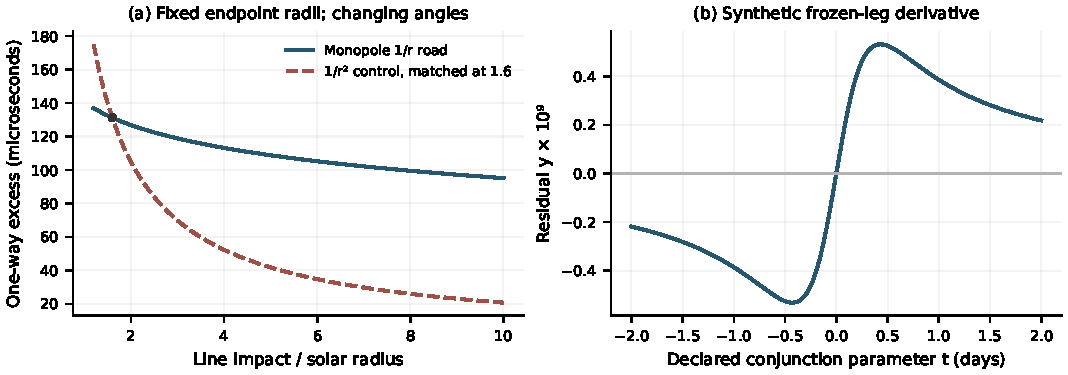
\includegraphics[width=\textwidth]{road_controls.pdf}
\caption{Declared controls, not tracking data. (a) The monopole road and an inverse-square control normalized at $b=1.6R_\odot$. Endpoint radii stay fixed; endpoint angles change. (b) A synthetic first-order residual $y=-2(\partial\Delta T_1/\partial b)\dot b$, using the frozen equal-leg approximation and $b(t)=\sqrt{b_0^2+v^2t^2}$ with $b_0=1.6R_\odot$ and $v=30$ km/s. The central delay is largest when its derivative vanishes. This parameterized curve is not a moving-endpoint two-way solution or a fit to Cassini ephemerides; actual leg epochs and baseline Doppler must be supplied for that task.}
\label{fig:roadcontrols}
\end{figure*}


\section{A shared source, two weak response coefficients}
The temporal and spatial responses can be parameterized independently before a source-native derivation is complete. Write
\[
 N^2=1-\kappa_t a+O(a^2),\qquad
 h_{ij}=[1+\kappa_s a+O(a^2)]\delta_{ij}.
\]
Direct expansion gives
\[
 N=1-\frac{\kappa_t}{2}a+O(a^2),\qquad
 n_{\rm opt}=1+\frac{\kappa_t+\kappa_s}{2}a+O(a^2).
\]
An endpoint comparison therefore measures the temporal coefficient, while a monopole timing route measures their sum. With one common source normalization, they imply $\kappa_s=2K_{\rm road}-2K_{\rm end}$, where $K_{\rm end}=\kappa_t/2$ and $K_{\rm road}=(\kappa_t+\kappa_s)/2$ are the coefficients of the same lift. In the declared metric used above, $\kappa_t=1$ and $\kappa_s=\gamma$.

This algebra makes a useful experimental and theoretical pairing: derive or measure the endpoint and route responses without independently rescaling their source amplitude. The Poisson kernel fixes the radial lift profile; it does not by itself choose either response coefficient. A spatial coefficient derived from the same retained action would supply the missing physical bridge.

\section*{Part C. The emitted carrier and amplitude transport}
\section{A propagation action connects phase and amplitude}
A concrete declared electromagnetic adapter is the minimally coupled action
\[
 S_{\rm EM}=-\frac14\int\sqrt{-g}\,g^{\mu\rho}g^{\nu\sigma}
 F_{\mu\nu}F_{\rho\sigma}\,\dd^4x.
\]
Its geometric-optics principal symbol gives $g^{\mu\nu}k_\mu k_\nu=0$ and the static optical metric $h_{ij}/N^2$. A local orthonormal observer measures $c$. A positive scalar multiplier $Z(x)$ leaves this cone unchanged while changing the leading flux equation to $\nabla_\mu(ZA^2k^\mu)=0$. Phase transport therefore does not fix amplitude transport.

For example, all members of the declared family
\[
 \dd s_\gamma^2=-(1-a)c^2\dd t^2+(1+\gamma a)|\dd\bm x|^2
\]
share the same stationary clock lapse where $0\le a<1$ and $1+\gamma a>0$. Their route indices are $\sqrt{(1+\gamma a)/(1-a)}$, and their first-order Shapiro coefficients differ. The cases $\gamma=0$ and $\gamma=1$ give respectively half and all of the retained road operator. This is a constructive separation of temporal and spatial information; it does not assert that all members solve one source field equation.

\section{A positive tensor action supplies an amplitude bridge}
Use $b_{\rm cos}(\eta_c)$ for the cosmological scale factor, normalized to one today, and $\mathscr H=b_{\rm cos}'/b_{\rm cos}$. The conformal time $\eta_c$ is distinct from the interacting clock's model-age variable. In units $c=1$, declare the two-polarization action
\[
\begin{aligned}
 S_T&=\frac12\sum_A\int\dd\eta_c\,\dd^3x\ b_{\rm cos}^2Q
 \left[(h_A')^2-c_T^2|\nabla h_A|^2\right],\\
 &\hspace{4em}Q>0,\qquad c_T^2>0.
\end{aligned}
\]
This is an explicit propagation construction by Codex, following the amplitude-friction representation retained in Ref.~[19]; $Q$ and $c_T$ are not assigned as source-native SAM coefficients. Its momentum and Hamiltonian are
\[
 \Pi_A=b_{\rm cos}^2Qh_A',\quad
 H_T=\frac12\sum_A\int\left[
 \frac{\Pi_A^2}{b_{\rm cos}^2Q}+b_{\rm cos}^2Qc_T^2|\nabla h_A|^2
 \right]\dd^3x.
\]
The instantaneous energy is nonnegative. Prescribed changes of the background coefficients supply external work; this is not a conserved total apparatus account.

Varying the action and Fourier transforming gives
\[
 h_A''+(2\mathscr H+Q'/Q)h_A'+c_T^2k^2h_A=0.
\]
Set $B=b_{\rm cos}\sqrt Q$ and $v_A=Bh_A$. Direct substitution cancels the first derivative and yields the exact equation
\[
 v_A''+\left[c_T^2k^2-\frac{B''}{B}\right]v_A=0.
\]
For $c_T=1$, a smooth high-frequency regime gives the leading amplitude $h_A\propto1/(b_{\rm cos}\sqrt Q)$ with the radial spreading factor. A quantitative use needs control of $|B''/B|/k^2$ and its variation on the chosen branch, with absorption and mode conversion included if present.

\section{Source, transport, detector and inferred distance}
If source generation and local detector normalization are matched between the comparison channels, the preceding transport amplitude gives
\[
\begin{aligned}
 \Xi(z)&=\frac{d_L^{\rm GW}}{d_L^{\rm EM}}
       =\sqrt{\frac{Q(0)}{Q(z)}},\\
 \delta(s)&=-\frac{\dd\ln\Xi}{\dd s}
       =\frac12\frac{\dd\ln Q}{\dd s},\qquad s=\ln(1+z).
\end{aligned}
\]
Here $Q(0)$ is the receiver value and $Q(z)$ the emitter value. Since $\dd s/\dd\eta_c=-\mathscr H$, the mode equation is $h_A''+2\mathscr H(1-\delta)h_A'+k^2h_A=0$, the amplitude-friction representation used in the finite-redshift paper.~[19] The amplitude factor is distinct from the principal phase speed $c_T$ and from a travel-time delay.

A source-generation or detector factor $G(z)$ changes the measured ratio to $Y(z)=C_{\rm cal}G(z)\Xi(z)$. The simpler $Y=C_{\rm cal}\Xi$ protocol requires $G$ to be controlled or fitted explicitly. Changing $c_T$ also changes the propagation problem; the displayed distance formula retains $c_T=1$ and the stated matching assumptions.

Conversely every smooth positive normalized $\Xi$ has a compatible positive coefficient
\[
 Q(z)=\frac{Q(0)}{\Xi(z)^2}.
\]
For $\Xi=\Xi_\infty+(1-\Xi_\infty)e^{-ps}$ with $p>0$ and $\Xi_\infty>0$, this gives
\[
 \delta(s)=\frac{p(1-\Xi_\infty)e^{-ps}}{\Xi_\infty+(1-\Xi_\infty)e^{-ps}}.
\]
Positivity of this declared action therefore selects neither a single power nor its exponent. An independently derived $Q$, $p$, or rate spectrum is the physical result needed from the common source dynamics.

The practical ratio additionally retains emission properties, inclination and polarization response, background distance, detector gain, opacity and selection. Independent angular-distance information can help separate channels: with $d_A$, define $\eta_{\rm EM}=d_L^{\rm EM}/[(1+z)^2d_A]$ and $\eta_{\rm GW}=d_L^{\rm GW}/[(1+z)^2d_A]$. Then $\Xi=\eta_{\rm GW}/\eta_{\rm EM}$, with ruler calibration and shared covariance retained. A trend in $\Xi$ alone does not determine which sector generated it.~[19]

\section{Finite-frequency amplitude and phase certificates}
The positive transport action now has an explicit finite-frequency estimate.
Write $B=b_{\rm cos}\sqrt Q>0$, $U=B''/B\in L^1[a,b]$, $c_T=1$, and retain the same incoming initial data for the canonical mode and its plane-wave comparator:
\[
 v(a)=1,\quad v'(a)=-\ii k,\qquad
 v_0(\eta_c)=e^{-\ii k(\eta_c-a)},\quad k>0.
\]
Variation of constants gives the exact equation
\[
 v=v_0+\int_a^{\eta_c}\frac{\sin[k(\eta_c-s)]}{k}U(s)v(s)\,\dd s.
\]
Set $M(\eta_c)=k^{-1}\int_a^{\eta_c}|U|\,\dd s$ and $\rho=e^M-1$. Gronwall, followed by substitution and differentiation, gives
\[
 |v-v_0|\le\rho,\qquad |v'-v_0'|\le k\rho.
\]
Indeed $|v(s)|\le e^{M(s)}$ and the resulting integral is exactly $e^{M(\eta_c)}-1$. No derivative bound on $U$ is needed. For $h=v/B$ and $h_0=v_0/B$,
\[
\begin{split}
 |h-h_0|&\le\rho/B,\\
 |h'-h_0'|&\le(k+|B'/B|)\rho/B.
\end{split}
\]
If $\rho<1$, the same disk gives
\[
 \big||v|-1\big|\le\rho,\qquad
 |\arg(v/v_0)|\le\arcsin\rho,
\]
with one continuous phase unwrapping from $a$. The real potential preserves $\operatorname{Im}(\bar v v')=-k$, so the actual phase rate is $-k/|v|^2$ and
\[
 \left|\frac{\dd\arg v}{\dd\eta_c}+k\right|
 \le k\big[(1-\rho)^{-2}-1\big].
\]
The positive factor $B$ changes no phase. These are separate amplitude, accumulated-phase and phase-rate certificates.

For a fully specified declared example, take $0\le\eta_c\le1$ and
\[
 b_{\rm cos}=\frac{10+\eta_c}{11},\qquad
 Q=\left(\frac{10+\eta_c}{10}\right)^2,\qquad k=100.
\]
Then $B=(10+\eta_c)^2/110$, $U=2/(10+\eta_c)^2$ and
\[
 M(1)=\frac1{5500},\qquad \rho(1)<\frac1{5499}.
\]
The last rational bound uses $e^x\le(1-x)^{-1}$ for $0\le x<1$. The leading endpoint factor is $B_E/B_R=100/121$, and the propagation-only distance ratio is $\sqrt{Q_R/Q_E}=11/10$. The finite-frequency amplitude disk is below $1.819\times10^{-4}$. This receiving example assigns no microscopic SAM $Q$ or physical conformal-time scale. An elementary exact basis,
\[
 w(\eta_c)=e^{-\ii k\eta_c}
 \left(1-\frac{\ii}{k(10+\eta_c)}\right),\quad\bar w,
\]
with Wronskian $2\ii k$, supplies the independent matched-initial-data check.

\section{Generation, propagation and detector normalization}
A source term $\mathcal J h$ in one normalized Fourier mode gives
\[
 (B^2h')'+B^2k^2h=\mathcal J,\qquad
 v''+(k^2-U)v=\mathcal J/B.
\]
For a zero incoming incremental mode and impulse $\mathcal J=j\delta(\eta_c-E)$, the canonical momentum jumps by $j$. If $G(R,E)$ has unit initial velocity and zero initial displacement, then
\[
 h(R)=\frac{jG(R,E)}{B_EB_R},\qquad
 W_{\rm impulse}=\frac{j^2}{2B_E^2}.
\]
Thus an equal source impulse and an equal emitted field preparation are different protocols when $Q_E$ differs.

Keep the preceding $b_{\rm cos}$ but set $Q=4[(10+\eta_c)/10]^2$. This leaves $U$ unchanged; now $Q_E=4$ and $Q_R=121/25$. Compare an electromagnetic mode with $Q=1$, the same $k=100$, and $E=0$, $R=1$. For $x_E=10$, $x_R=11$ and $L=1$, the complete retarded Green functions are
\[
\begin{split}
 G={}&\left(1+\frac1{k^2x_Ex_R}\right)\frac{\sin kL}{k}\\
 &+\left(\frac1{x_R}-\frac1{x_E}\right)\frac{\cos kL}{k^2},\\
 G_{\rm EM}={}&\frac{\sin kL}{k}.
\end{split}
\]
Here $G/G_{\rm EM}=1.0001557233563114\ldots$ at this specified nonzero readout. The absolute Green error also satisfies $k|G-G_{\rm EM}|\le e^M-1$; no ratio is assigned at a zero of $G_{\rm EM}$.

Let $d$ be the receiving detector-gain ratio. The recorded amplitudes obey exactly
\[
 \frac{A_T}{A_{\rm EM}}=
 d\frac{j_T}{j_{\rm EM}}\frac1{\sqrt{Q_EQ_R}}
 \frac{G}{G_{\rm EM}}.
\]
Equal impulses and $d=1$ give $(5/22)(G/G_{\rm EM})$. Matching the emitted $h'$ requires $j_T=Q_Ej_{\rm EM}=4j_{\rm EM}$ and gives $(10/11)(G/G_{\rm EM})$. A detector gain $d=3/2$ changes the latter to $(15/11)(G/G_{\rm EM})$. The inferred amplitude distances are the reciprocal ratios. Only the matched-emission, matched-detector protocol has the leading propagation-only ratio $11/10$.

For $j_{\rm EM}=1$, the electromagnetic impulse costs $121/200$ per normalized mode; the equal-impulse tensor mode costs $121/800$; matched emission costs $121/50$. During propagation the prescribed background also does signed work:
\[
 \frac{\dd H}{\dd\eta_c}
 =BB'k^2h^2-\frac{B'}{B^3}\Pi^2
\]
for each real mode outside the impulse. Source preparation, prescribed-background work and a detector's absorbing or disturbing measurement remain in their respective accounts. The displayed linear detector gain is a declared receiving convention.

\section{The original causal tensor carrier as a signal map}
The next calculation returns to the actual retained quadrupole TT carrier, distinct from the preceding electromagnetic and cosmological adapters. Keep its two signed source quadratures, $\kappa=4/5$, $c_*=1$, regular interior, full outgoing exterior and original radius $R$. For $r=\varrho R$, $\varrho\ge1$, let
\[
\begin{split}
 s(w)&=(r+Rw)/c_*,\\
 K_{\varrho}(w)&=\frac1{\kappa\varrho}
 P_2\!\left(-w+\frac{1-w^2}{2\varrho}\right).
\end{split}
\]
The complete driven receiver is
\[
 x_{\rm out}(t)=\int_{-1}^{1}K_{\varrho}(w)f(t-s(w))\,\dd w.
\]
A homogeneous incoming/prepared field adds its own receiver term. The retained maintained-pulse experiment has zero incremental incoming field on the same stationary reference; the full background and field energy remain. The frequency response is
\[
 \chi(\omega)=\frac{2\ii z}{\kappa}j_2(z)h_2^{(1)}(z\varrho),
 \qquad z=\omega R/c_*.
\]
All near, induction and radiation terms are retained. The first and last kernel supports are $(r-R)/c_*$ and $(r+R)/c_*$. On the original small-frequency branch $j_2(z)>0$, the group delay is
\[
 \tau=\frac r{c_*}
 \frac{u^4}{u^4+3u^2+9},\qquad u=\omega r/c_*.
\]
A signed kernel can have a group delay outside its causal support interval; the two observables remain distinct.

For a carrier-modulated envelope $f=a(t)e^{-\ii\omega_0t}$, choose $\chi_0=\chi(\omega_0)\ne0$ and $\tau=(\dd\arg\chi/\dd\omega)|_{\omega_0}$. The gain/delay approximation is
\[
 x_{\rm app}=\chi_0e^{-\ii\omega_0t}a(t-\tau).
\]
More explicitly, write $\tau=(\dd/\dd\omega)\arg\chi|_{\omega_0}$ and define
\[
\begin{split}
 L_1&=|\chi'(\omega_0)-\ii\tau\chi_0|,\\
 D_2&=\int |K_{\varrho}(w)|[s(w)-\tau]^2\,\dd w.
\end{split}
\]
Taylor's remainder for $e^{\ii\nu(s-\tau)}$ gives
\[
 |\chi(\omega_0+\nu)-\chi_0e^{\ii\nu\tau}|
 \le |\nu|L_1+\tfrac12\nu^2D_2.
\]
If the envelope spectrum lies in $|\nu|\le\beta$, Plancherel gives
\[
 \|x_{\rm out}-x_{\rm app}\|_2
 \le(\beta L_1+\tfrac12\beta^2D_2)\|a\|_2.
\]
The first term is amplitude dispersion: at the stated group delay $L_1=|\dd|\chi|/\dd\omega|$. For a bounded smooth envelope, direct Taylor expansion instead gives the pointwise bound
\[
 |x_{\rm out}-x_{\rm app}|
 \le L_1\|a'\|_\infty+\tfrac12D_2\|a''\|_\infty.
\]
This version needs no frequency truncation, and applies to a compact pulse.

\section{A complete source pulse and a nonzero phase event}
Retain the actual four-cycle source
\[
 f_{ab}(t)=g_{ab}A(\Delta t)e^{-\ii\Delta t},\qquad
 \Delta=\frac2{573049},
\]
where $A(\theta)=\sin^4(\theta/8)$ on $[0,8\pi]$ and zero outside. The six signed $g_{ab}$, equal pair weights $1/6$, both tensor polarizations, four undriven source diagonal states and complete maintenance-work account are unchanged. The envelope is $C^3$ with bounded fourth weak derivative.

The complete signed delay moments satisfy
\[
\begin{split}
 m_0&=\frac2{5\kappa\varrho^3},\quad m_1=m_3=0,\\
 \frac{m_2}{m_0}&=\frac{R^2}{7c_*^2}-\frac{r^2}{3c_*^2},\quad
 m_n=\int K_{\varrho}s^n\,\dd w.
\end{split}
\]
These follow by expanding the full argument of $P_2$ and integrating monomials. At $\varrho=2$, with $(R/c_*)^n$ factored out, moments zero through four are
\[
 (1/16,\ 0,\ -25/336,\ 0,\ 313/336).
\]
Thus odd-moment cancellation and a negative signed second moment quantify the near-field behavior.

Taylor's formula, including both compact-pulse edges, gives
\[
\begin{split}
 |x_{\rm out}-m_0f|
 &\le\frac{|m_2|}2\|f''\|_\infty
       +\frac{D_4}{24}\|f^{(4)}\|_\infty,\\
 D_4&=\int|K_{\varrho}|s^4\,\dd w
 \le\frac{2(r+R)^4}{\kappa\varrho c_*^4}.
\end{split}
\]
For $\varrho\ge1$, the Legendre argument maps $[-1,1]$ monotonically onto $[1,-1]$, so $|P_2|\le1$. The exact five-frequency interior expansion gives
\[
 \|f''\|_\infty\le|g|\Delta^2\frac{17}{16},\qquad
 \|f^{(4)}\|_\infty\le|g|\Delta^4\frac{709}{512}.
\]
The zero extension has the same weak-derivative bounds. No frequency or radial tail is cut.

At the original receiver $r=R+64$, use the complete authenticated Chapter I radius ball, rather than treating a printed decimal as exact. Outward rational arithmetic yields, for every time and every original signed lane,
\[
 \frac{|x_{\rm out}-m_0f|}{m_0|g|}<8.994\times10^{-9}.
\]
Also $|\chi(\Delta)-m_0|/m_0<8.440\times10^{-9}$ and
\[
 0<\tau<1.792884\times10^{-14}
\]
in original model-time units, while first causal arrival remains exactly $64$. Replacing the static gain by the full monochromatic gain and its group delay gives
\[
 \frac{\left|x_{\rm out}-g\chi(\Delta)e^{-\ii\Delta t}
 A[\Delta(t-\tau)]\right|}{m_0|g|}
 <1.744\times10^{-8}.
\]
This is a uniform absolute-envelope error normalized by peak static gain. A phase disk requires a positive received envelope: if $A[\Delta(t-\tau)]\ge a_*>0$, its radius is at most
\[
 \arcsin\!\left[\frac{\epsilon_{\rm pulse}}
 {a_*(1-\epsilon_{\rm gain})}\right],
\]
when the argument is below one. It supplies no phase statement at zeros.

A sharper phase certificate is available at the actual peak event $t_*=4\pi/\Delta$. Every retarded source argument then lies inside the smooth pulse. After demodulation and division by signed $g$,
\[
 Y=\int K_{\varrho}(w)e^{\ii\Delta s}
       \cos^4(\Delta s/8)\,\dd w.
\]
The sine expansion has positive weights and relative frequencies
\[
 \begin{aligned}
 \text{Weights}:\;&(3/8,1/4,1/4,1/16,1/16),\\
 \text{Frequency ratios}:\;&(1,5/4,3/4,3/2,1/2).
 \end{aligned}
\]
Their fifth-derivative sum is $857/512$. Since $m_1=m_3=0$,
\[
 \begin{aligned}
 |\operatorname{Im}Y|&\le\frac{857}{512}\frac{\Delta^5D_5}{120},\\
 |\operatorname{Im}\chi|&\le\frac{\Delta^5D_5}{120},
 \end{aligned}
\]
where $D_5\le2(r+R)^5/(\kappa\varrho c_*^5)$. The preceding real-part lower bounds then give
\[
\begin{split}
 |\arg Y-\arg\chi|\le{}&\frac{\Delta^5D_5}{120m_0}
 \left[\frac{857/512}{1-\epsilon_{\rm static}}
       +\frac1{1-\epsilon_{\rm gain}}\right]\\
 <{}&9.782\times10^{-15}\ \text{radians}.
\end{split}
\]
The gain/delay comparator's envelope is positive at this event and changes no phase. This is one nonzero-amplitude phase event; timing, incoming-field contamination, detector disturbance and statistical error remain in the measurement protocol. Source maintenance, free/drive/counterterm energy and complete emitted-field energy remain in the retained ledger.

\section{The original carrier from the near field to radiation}
\label{sec:actual-radiation-zone}
The user-supplied review derived the exact decomposition and compact-edge
remainder below. An independent calculation from the retained complete kernel
agrees. The flux estimate and finite-endpoint examples extend that derivation.
The original six signed $g_{ab}$, equal pair weights, both tensor polarizations,
$\kappa=4/5$, radius balls and $\Delta=2/573049$ remain fixed.

Put $a=R/c_*$, $v=r/R\geq1$, $t_r=t-r/c_*$ and
$x_r=R\phi(r,t)$. Polynomial expansion gives
\begin{align}
 P_2\!\left[-w+\frac{1-w^2}{2v}\right]
 &=P_2(w)-\frac{3w(1-w^2)}{2v}
             +\frac{3(1-w^2)^2}{8v^2},\\
 x_r&=x_{\rm rad}+x_{\rm ind}+x_{\rm near},\nonumber\\
 x_{\rm rad}&=\frac1{\kappa v}\int_{-1}^1P_2(w)f(t_r-aw)\,dw,\nonumber\\
 x_{\rm ind}&=-\frac3{2\kappa v^2}\int_{-1}^1w(1-w^2)f(t_r-aw)\,dw,\nonumber\\
 x_{\rm near}&=\frac3{8\kappa v^3}\int_{-1}^1(1-w^2)^2f(t_r-aw)\,dw.
 \label{eq:exact-three-radial-pieces}
\end{align}
These are exact $r^{-1}$, $r^{-2}$ and $r^{-3}$ pieces at fixed retarded time.
All have the original causal support $[(r-R)/c_*,(r+R)/c_*]$.
The unchanged homogeneous incoming field is added separately. The normalized
angular tensor remains $\sqrt{5/(8\pi)}\Lambda_n$ applied to the original
plus/cross source; its sphere isometry fixes the angular amplitude ruler.

\subsection{A whole-pulse derivative and remainder theorem}
For $f\in C^3(\mathrm R)$ with bounded fourth weak derivative, parity and
Taylor's integral remainder yield
\begin{align}
 x_r(t)&=\frac{2R^3}{15\kappa}
 \left[\frac{f''(t_r)}{c_*^2r}
       +\frac{3f'(t_r)}{c_*r^2}+\frac{3f(t_r)}{r^3}\right]+E(t),\\
 |E(t)|&\leq\frac{a^4\|f^{(4)}\|_\infty}{60\kappa v}
       +\frac{a^3\|f'''\|_\infty}{35\kappa v^2}
       +\frac{a^2\|f''\|_\infty}{35\kappa v^3}.
 \label{eq:compact-edge-radiation-remainder}
\end{align}
For example, the radiative coefficient uses
$\int P_2=0$ and $\int w^2P_2=4/15$; its remainder follows from
$\int |P_2|w^4\leq2/5$. The induction and near remainders use respectively
$\int w^4(1-w^2)=4/35$ and
$\int w^2(1-w^2)^2=16/105$. These estimates apply on the zero extension,
including intervals that cross either pulse edge.

The actual maintained pulse is $f=g_{ab}F(\Delta t)$, with
$F(\theta)=\sin^4(\theta/8)e^{-i\theta}$ on $[0,8\pi]$ and zero elsewhere.
Its first three derivatives match zero at both endpoints. Its five-frequency
expansion gives
\[
 \begin{gathered}
 \|f^{(j)}\|_\infty\leq |g_{ab}|\Delta^jD_j,\\
 (D_0,D_1,D_2,D_3,D_4)
   =\left(1,1,\frac{17}{16},\frac{19}{16},\frac{709}{512}\right).
 \end{gathered}
\]
Define $z=\Delta R/c_*$, $u=\Delta r/c_*$ and the specified positive ruler
$A_0=2R^3|g_{ab}|\Delta^2/(15\kappa c_*^2r)$. Then, for every time,
\begin{equation}
 \begin{aligned}
 &\frac{|x_r-A_0\operatorname{sgn}(g_{ab})F''(\Delta t_r)|}{A_0}\\
 &\quad\leq\frac3u+\frac3{u^2}\\
 &\qquad+z^2\left(\frac{709}{4096}+\frac{57}{224u}
                               +\frac{51}{224u^2}\right).
 \end{aligned}
 \label{eq:radiation-ruler-bound}
\end{equation}
This is an absolute curve bound; phase and relative error need a nonzero
comparator. The full original radius ball gives $z<5.708\times10^{-7}$.
For $u=100,1000,10^6$, the right side is below
$0.030300000001$, $0.003003000001$ and $0.0000030000031$.
These correspond to $r=u/\Delta$ in the same $c_*=1$ model chart.
The old receiver $r=R+64$ has $u<0.000224$.

At the retarded envelope peak $\theta=4\pi$, $F''=-17/16$ is real.
The leading radiative peak therefore has a $6.25\%$ amplitude correction,
with the same phase, relative to a central-frequency unchanged-envelope
approximation. Increasing $r$ leaves that waveform correction present.
The four-cycle maintained pulse and the one-cycle autonomous clock retain
their different source protocols.

\subsection{A finite-radius amplitude ruler and positive emitted energy}
The exact monochromatic identity is
\begin{align}
 \chi_r&=-\frac{2j_2(z)e^{iu}}{\kappa v}
                 \left(1+\frac{3i}{u}-\frac3{u^2}\right),\\
 \chi_{\rm rad}&=-\frac{2j_2(z)e^{iu}}{\kappa v},\\
 \left|\frac{\chi_r}{\chi_{\rm rad}}\right|^2
 &=1+\frac3{u^2}+\frac9{u^4},\\
 \left|\frac{\chi_r}{\chi_{\rm rad}}-1\right|
 &\leq\frac3{|u|}+\frac3{u^2}.
\end{align}
The ratio requires $j_2(z)\ne0$. At $u=100$ the amplitude excess is below
$0.000150045$; the induction term still contributes an order $1/u$ phase.
The local detector functional, angular projection, gain, original source
vertex and $1/r$ factor all enter the recorded amplitude ruler.

The exact coefficient at null infinity and its energy are
\begin{align}
 \psi(t_r)&=\lim_{r\to\infty}r\phi(r,t_r+r/c_*)
       =\frac1\kappa\int_{-1}^1P_2(w)f(t_r-aw)\,dw,\\
 W&=\frac{\kappa}{2c_*}\int_{\mathrm R}|\psi'|^2dt_r.
\end{align}
For $\psi_0=2a^2f''/(15\kappa)$, the comparator is
\[
 W_0=\frac{2R^4g_{ab}^2\Delta^5I_3}{225\kappa c_*^5}.
\]
% Insert within the existing original-carrier section, after W and W_0 are
% defined in radiation_local.tex, replacing the conservative energy paragraph.
\subsection{Exact smoothing fixes the integrated energy sign}
\label{subsec:signed-radiative-energy-update}
The owner's six-page review supplies a sharper theorem for the same
maintained pulse. It keeps both original compact edges and all six signed
source vertices. Put $a=R/c_*$ and let
\[
 \mu(w)=\begin{cases}
  \frac{15}{16}(1-w^2)^2,&|w|\leq1,\\
  0,&|w|>1.
 \end{cases}
\]
Its mass, mean and variance are $1$, $0$ and $1/7$. Since
$P_2(w)=[(1-w^2)^2]''/8$, the two endpoint terms vanish under two
integrations by parts; the equivalent spherical Bessel normalization is also given by DLMF 10.54.1.~[20] Thus the \emph{exact} outgoing radiation is
\[
 \psi=\frac{2a^2}{15\kappa}\mathcal C_\mu f'',\qquad
 \psi'=\frac{2a^2}{15\kappa}\mathcal C_\mu f''',
\]
where $(\mathcal C_\mu g)(t)=\int\mu(w)g(t-aw)\,dw$.
For any $g$ with $g,g'\in L^2$, polarization gives
\begin{align*}
 \|g\|_2^2-\|\mathcal C_\mu g\|_2^2
 &=\frac12\iint\mu(w)\mu(v)\\[-2pt]
 &\quad\times\|g(\cdot-aw)-g(\cdot-av)\|_2^2\,dw\,dv\\
 &\leq\frac{a^2}{7}\|g'\|_2^2.
\end{align*}
The last inequality uses the Sobolev translation bound and
$\int\!\int\mu(w)\mu(v)(w-v)^2\,dw\,dv=2/7$.
The original zero-extended pulse is $C^3$ across its endpoints, so
$g=f'''$ has weak derivative $g'=f^{(4)}\in L^2$. Its original
five-frequency expansion gives
\[
 \begin{aligned}
 I_3&=\int_0^{8\pi}|F'''|^2d\theta=\frac{14245\pi}{4096},\\
 I_4&=\int_0^{8\pi}|F^{(4)}|^2d\theta=\frac{324817\pi}{65536}.
 \end{aligned}
\]
Consequently the same $W,W_0$ satisfy
\begin{align}
 0\leq1-\frac W{W_0}
 &\leq\frac{a^2\|f^{(4)}\|_2^2}{7\|f'''\|_2^2}
   =\frac{324817}{1595440}z^2\nonumber\\
 &<6.633\times10^{-14},\qquad z=\Delta R/c_*.
 \label{eq:signed-energy-deficit-update}
\end{align}
The numerical upper endpoint uses the full original radius ball.
Finite-source smoothing therefore reduces this integrated energy relative
to the derivative comparator. It is a signed certificate for the original
maintained pulse; it changes neither the autonomous-clock preparation nor
its source-depletion account. The common ratio retains each lane's signed
waveform and cancels only its common squared vertex in $W/W_0$.

\subsection{Exact source work, sphere flux and near-field storage}
The supplied review asks for an all-time conservation check for the maintained
incremental pulse. A direct calculation from the original kernel gives it.
Let $a=R/c_*$ and $\mu(w)=15(1-w^2)^2/16$ on $[-1,1]$, and set
\[
 A(u)=\frac{2R^2}{15\kappa c_*^2}
       \int\mu(w)f(u-aw)\,dw,\qquad u=t-r/c_*.
\]
Two integrations by parts give the exact exterior solution
\[
 \phi(r,t)=\frac{A''(u)}r+\frac{3c_*A'(u)}{r^2}
                       +\frac{3c_*^2A(u)}{r^3}.
\]
This includes both compact-pulse edges. Write $q_j=A^{(j)}(u)$ and
$y=(q_2,c_*q_1/r,c_*^2q_0/r^2)$. The complete outward sphere flux is
\[
 \begin{gathered}
 F_r(t)=\frac{\kappa}{2c_*}|q_3|^2+\frac{dS_r(u)}{dt},\\
 S_r=\frac{\kappa}{2r}y^*G y,\qquad
 G=\begin{pmatrix}7/2&6&9/2\\6&15&27/2\\9/2&27/2&27/2\end{pmatrix}.
 \end{gathered}
\]
Its exact LDL pivots are $7/2,33/7,27/44$, all positive. Thus $S_r$ is
nonnegative stored near-field energy on the outgoing characteristic; its
derivative can have either sign. The instantaneous sphere flux need not be
positive. The full exterior energy is
\[
 E_{>r}(t)=\frac{\kappa}{2c_*}\int_{-\infty}^{u}|A'''(v)|^2dv+S_r(u).
\]
Since $A$ is compactly supported, every exterior sphere has the same
all-time integrated flux $W=\kappa\int|A'''|^2/(2c_*)$.

The original radial energy density and flux are
\[
 \begin{gathered}
 e=\frac\kappa4\left[\frac{r^2|\phi_t|^2}{c_*^2}
                     +r^2|\phi_r|^2+6|\phi|^2\right],\\
 F_r=-\frac\kappa2r^2\operatorname{Re}(\phi_t^*\phi_r).
 \end{gathered}
\]
Their local continuity equation and the original source jump give
$\dot E_{<b}+F_b=\operatorname{Re}(f^*\phi_t(R))$ for $b>R$.
Keep $H_{\rm drive}=-\operatorname{Re}(f^*\phi(R))$ and
$H_{\rm ct}=|f|^2/(4R)$ in the actual tensor sector. Explicit control power is
\[
 P_{\rm ctrl}=-\operatorname{Re}(\dot f^*\phi(R))+\dot H_{\rm ct}.
\]
Hence
\[
 \frac d{dt}(E_{<b}+H_{\rm drive}+H_{\rm ct})+F_b=P_{\rm ctrl}.
\]
The maintained source's even energy is constant; any different source-energy
change must be added to its recipient and power account. With zero incoming
field and zero force endpoints, the completed net control work equals $W$,
the integrated flux through every $b>R$, and the full outgoing exterior
energy. Intermediate interaction and counterterm changes remain explicit.
Signed endpoint cancellation supplies no zero-apparatus-cost assertion.

For nonzero incoming field, retain the incoming, emitted and bilinear cross
terms in both energy and flux, including
$\operatorname{Re}(f^*\phi_{{\rm in},t}(R))$ in source power. The frozen native storage check retains the cross block for two outgoing
jets. A separate exact bidirectional checker uses the inward exterior
solution $\phi_{\rm in}=A_{\rm in}''/r-3c_*A_{\rm in}'/r^2+
3c_*^2A_{\rm in}/r^3$ and verifies pure and cross continuity and signed
radiative flux. A regular incoming background also has its matching
outgoing component; an inward characteristic alone is only local to the exterior. This maintained classical carrier
identity remains distinct from autonomous quantum-source depletion.

The exact flux, full outgoing exterior, incoming preparation, source work,
boundary interaction, counterterm and even source/reference energy remain in
the ledger. This fixed flat-carrier normalization supplies no cosmological
$Q$, redshift-dependent generation function or SI conversion by itself.

\section{The canonical electromagnetic comparison}
\label{sec:maxwell-canonical-comparator}
For one transverse conformal Maxwell mode use
$L_M=(A'^2-k^2A^2)/2$. The earlier $Q=1$ comparator uses $h=A/b$ and
$L_h=b^2(h'^2-k^2h^2)/2$. With $\mathcal H=b'/b$,
\begin{align}
 L_h&=\frac12\left[A'^2-
              \left(k^2-\frac{b''}{b}\right)A^2\right]
                   -\frac12(\mathcal H A^2)',\\
 J_hh&=\frac{J_h}{b}A,\qquad j_A=\frac{j_h}{b_E},\\
 D_hh_R&=\frac{D_h}{b_R}A_R.
\end{align}
For the displayed linear $b$, $b''=0$, so these are the same free equations
with the stated canonical boundary term, source and detector transformations.
Their energies satisfy
\[
 \begin{gathered}
 E_h-E_M=-\mathcal H AA'+\tfrac12\mathcal H^2A^2,\\
 E_h=\tfrac12[(A'-\mathcal H A)^2+k^2A^2].
 \end{gathered}
\]
An impulse from zero field has the common work
$j_h^2/(2b_E^2)=j_A^2/2$, recovering the earlier impulse numbers under this
protocol. At nonzero incoming $A$, the two impulse work changes differ by
$-\mathcal H A j_A$; that term belongs to the boundary/background account.
A fixed Maxwell impulse or detector gain requires the corresponding
transformed $h$ values. This specifies the electromagnetic comparison of
the linear-$b$ example.

\section{Moving endpoints of the actual travel-time map}
\label{sec:moving-travel-time-gradient}
Let a differentiable one-branch travel-time function define actual events by
\[
 F(t_E)-t_E=T[t_E,x_E(t_E),F(t_E),x_R(F(t_E))].
\]
Implicit differentiation yields the review's event Jacobian, including
explicit reception-time dependence when present:
\begin{equation}
 F'=\frac{1+\partial_ET+\nabla_ET\cdot v_E}
          {1-\partial_RT-\nabla_RT\cdot v_R}.
 \label{eq:full-moving-event-jacobian}
\end{equation}
The chosen forward causal branch has a nonzero denominator and $F'>0$.
For stationary isotropic optics, endpoint variation gives
$\nabla_ET=-p_E$, $\nabla_RT=p_R$, with optical slowness
$p=n_{\rm opt}\widehat t/c_*$.
The velocities and gradients use their different actual event epochs.
With worldline proper rates $a_A=d\tau_A/dt$ and intrinsic interacting-clock
rates $\nu_A(\tau_A)$, the observed frequency comparison is
\[
 \mathcal R=\frac{a_E\nu_E(\tau_E)}{a_RF'\nu_R(\tau_R)}.
\]
The interacting transient and proper ages stay in this expression. The
actual delay derivative along events is $dT/dt_E=F'-1$.

For the retained weak-source, finite-endpoint logarithm let
$D=|x_R-x_E|$, $A=r_E+r_R$, $n=(x_R-x_E)/D$,
$e_A=x_A/r_A$ and $K=(1+\gamma)GM/c_*^3$. Then
\begin{align}
 T_{\rm app}&=D/c_*+K\log\frac{A+D}{A-D},\\
 \nabla_ET_{\rm app}
 &=-n/c_*-\frac{2K(De_E+An)}{A^2-D^2},\\
 \nabla_RT_{\rm app}
 &= n/c_*+\frac{2K(An-De_R)}{A^2-D^2}.
\end{align}
These gradients enter the actual implicit map. The travel-time approximation
retains its metric-order error. More quantitatively, write its numerator and
denominator as $A_*,B_*$. If $B_{\rm app}\geq b>\delta_B$,
$|A_*-A_{\rm app}|\leq\delta_A$ and
$|B_*-B_{\rm app}|\leq\delta_B$, then
\[
 |F'-F'_{\rm app}|\leq
 \frac{\delta_A}{b-\delta_B}
 +\frac{|A_{\rm app}|\delta_B}{b(b-\delta_B)}.
\]
The operands include path-gradient and endpoint-velocity uncertainties.
Compose outgoing, proper-wait and return maps at their actual event epochs.

\section{A signed finite-frequency transport correction}
For the retained Volterra equation $v=v_0+Vv$ put $v_1=Vv_0$ and
$M=\int|U|/k$. Ordered integration gives
$\|V^nv_0\|_\infty\leq M^n/n!$, hence
\[
 v=v_0+v_1+R_2,\qquad |R_2|\leq e^M-1-M.
\]
The same remainder controls the derivative divided by $k$. A nonzero lower
bound for $|v_0+v_1|$ turns this disk into amplitude and phase bounds about
the signed first correction. In the retained $M=1/5500$ example,
$|R_2|\leq M^2/[2(1-M)]<1.654\times10^{-8}$.
The source-derived physical transport coefficient remains its own calculation.


\section*{Part D. What a measured distance curve determines}
\section{A calibrated ratio on a finite interval}
Let $u=1+z$, $s=\ln u$, and adopt the normalized single-power distance family
\[
 \Xi(z)=\Xi_\infty+(1-\Xi_\infty)u^{-p},\qquad p>0.
\]
The measured ratio includes an unknown constant relative calibration,
\begin{equation}
 Y(z)=C_{\rm cal}\Xi(z)=\alpha+\beta e^{-ps},\quad
 C_{\rm cal}=\alpha+\beta,\quad
 \Xi_\infty=\frac{\alpha}{\alpha+\beta}.
 \label{eq:single-power}
\end{equation}
The symbol $\Xi_\infty$ denotes the plateau within this family; it is the $\Xi_0$ notation of the finite-redshift source.~[19] The calibration $C_{\rm cal}$ is an extrapolated relative distance scale at $z=0$ when the normalization $\Xi(0)=1$ is used. The calibration subscript distinguishes this quantity from the source current operator $C$ of the clock sections.

A constant gain can be fitted with $\alpha,\beta$. Redshift-dependent calibration requires a model or independent information: $Y=C_{\rm cal}(s)\Xi(s)$ is invariant under $\Xi\mapsto f\Xi$, $C_{\rm cal}\mapsto C_{\rm cal}/f$. Background luminosity distance, channel propagation and calibration are consequently different physical operands even when they enter one ratio.

A directly finite-window quantity avoids endpoint extrapolation. For positive ratios,
\[
 \overline\delta_{ij}=-\frac{\ln[Y(z_j)/Y(z_i)]}{s_j-s_i}.
\]
A constant calibration cancels. Under an amplitude-friction representation $\delta=-\dd\ln\Xi/\dd s$, this is its exact interval average. With small ratio errors and covariance $\Sigma$,
\[
 \Var(\overline\delta_{ij})\simeq
 \frac{\Sigma_{ii}/Y_i^2+\Sigma_{jj}/Y_j^2-2\Sigma_{ij}/(Y_iY_j)}{(s_j-s_i)^2}.
\]
This quantity tests measured evolution while retaining the two-channel covariance.

\section{Two samples recover the declared linear part}
At a specified $p$, set $x_i=u_i^p$. Since $xY=\alpha x+\beta$, two distinct exact samples give
\[
 \alpha=\frac{x_jY_j-x_iY_i}{x_j-x_i},\qquad
 \beta=\frac{x_ix_j(Y_i-Y_j)}{x_j-x_i}.
\]
The calibration and normalized plateau follow from Eq.~\eqref{eq:single-power} if $C_{\rm cal}\ne 0$. The differential projection $Y+(u/p)\dd Y/\dd u=\alpha$ states the same two-dimensional function-space identity; finite-sample algebra avoids differentiating noisy data. These are exact recovery formulas within the family, not a separate test of that family.~[19]

\section{Three samples determine a positive exponent}
For $s_0<s_1<s_2$, put $h_1=s_1-s_0$, $h_2=s_2-s_1$ and
\[
 r=\frac{Y_2-Y_1}{Y_1-Y_0},\qquad
 F(p)=\frac{1-e^{-ph_2}}{e^{ph_1}-1}.
\]
A nonconstant single-power member obeys $r=F(p)$. The function decreases strictly from $h_2/h_1$ to zero. Hence $0<r<h_2/h_1$ is necessary and sufficient for a unique positive exponent fitting the three exact samples.

\noindent\textit{Proof of strictness.} Logarithmic differentiation gives
\[
 \frac{F'(p)}{F(p)}=
 \frac{h_2}{e^{ph_2}-1}-\frac{h_1}{1-e^{-ph_1}}<0,
\]
because the first term is smaller than $1/p$ and the second is larger than $1/p$. The endpoint limits follow from expansion at zero and exponential decay at infinity. Continuity and strict monotonicity give existence and uniqueness. Solving the first two samples then supplies $\alpha,\beta$. Membership in the positive-distance family also requires the reconstructed $C_{\rm cal}=\alpha+\beta>0$ and $\Xi_\infty=\alpha/C_{\rm cal}>0$; the exponent criterion itself is the algebraic reconstruction statement.

For equal logarithmic spacing $s_j=s_0+jh$, let $\lambda=e^{-ph}$. Then
\[
\begin{aligned}
 \lambda&=\frac{Y_2-Y_1}{Y_1-Y_0},\qquad p=-\frac{\ln\lambda}{h},\\
 \alpha&=\frac{Y_0Y_2-Y_1^2}{Y_0-2Y_1+Y_2},\qquad
 \beta=(Y_0-\alpha)e^{ps_0}.
\end{aligned}
\]
Near a constant response or a nearly vanished transient, the denominators reveal poor conditioning. Three exact points reconstruct a member; a fourth supplies a consistency condition.~[19]

\section{A fourth sample tests the single-power shape}
Let $d_i=Y_{i+1}-Y_i$ and $h_i=s_{i+1}-s_i$. Define
\[
 F_{i,i+1}(p)=\frac{1-e^{-ph_{i+1}}}{e^{ph_i}-1}.
\]
The two triplets require the same positive exponent:
\[
 F_{01}^{-1}(d_1/d_0)=F_{12}^{-1}(d_2/d_1).
\]
For noisy data, use increments without dividing by a small increment:
\[
 g(p)=\begin{pmatrix}d_1-F_{01}(p)d_0\\d_2-F_{12}(p)d_1\end{pmatrix}.
\]
Its covariance is obtained by applying the same linear contrast to the full ratio covariance. At equal spacing the exact condition reduces to the Hankel determinant $H=d_0d_2-d_1^2=0$. These formulas require point samples or common translated bin windows; unequal windows must use Appendix~\ref{app:statistics}'s window-aware exponential templates before any single-mode or rank interpretation.

For two distinct geometric modes, $Y_j=\alpha+B_1\lambda_1^j+B_2\lambda_2^j$, direct expansion gives
\[
 H=B_1B_2(\lambda_1-1)(\lambda_2-1)(\lambda_1-\lambda_2)^2.
\]
This identifies precisely when a second mode produces a nonzero four-point departure. It also shows why close mode rates or a weak second amplitude give small departures. The statistical covariance and profiling treatment are retained in Appendix~\ref{app:statistics}.~[19]

\section{Positive response modes and finite rank}\label{sec:positive-modes}
The single-power test extends to a declared positive finite response class. All following Hankel identities assume point samples or common translated bin windows. Unequal windows require Appendix~\ref{app:statistics}'s window-aware treatment; one true mode can otherwise fail the single-mode identity.
On an equally spaced logarithmic grid $s_j=s_0+jh$, suppose
\begin{equation}
 Y_j=\alpha+\sum_{a=1}^r B_a\lambda_a^j,
 \qquad B_a>0,\quad 0<\lambda_a<1,
 \label{eq:positive-modes}
\end{equation}
with distinct nodes. Here $\lambda_a=e^{-p_a h}$ and $B_a$ includes the
initial-grid factor. These are inference assumptions; their identification
with a spectral measure of the physical source remains a separate derivation.
For $e_j=Y_j-Y_{j+1}$ and $w_a=B_a(1-\lambda_a)$,
\begin{equation}
 \begin{gathered}
 (H_m)_{ij}=e_{i+j},\qquad (V_m)_{ia}=\lambda_a^i,\\
 H_m=V_m\operatorname{diag}(w_a)V_m^T.
 \end{gathered}
 \label{eq:positive-hankel}
\end{equation}
Positivity and the Vandermonde minors give
$H_m\succeq0$ and $\operatorname{rank}H_m=\min(m,r)$.
A positive $r$-square determinant therefore detects at least $r$ visible
modes. An increasing branch has the same result after reversing all
differences when its amplitudes have a common opposite sign. Mixed signed
amplitudes require another analysis.

Write $p(x)=\prod_a(x-\lambda_a)=x^r+\sum_{k<r}c_kx^k$.
The moment recurrence and reconstruction system are
\begin{equation}
 \begin{gathered}
 e_{j+r}+\sum_{k<r}c_ke_{j+k}=0,\\
 H_r\bm c=-(e_r,\ldots,e_{2r-1})^T.
 \end{gathered}
 \label{eq:prony-system}
\end{equation}
Thus $2r+1$ exact $Y$ samples reconstruct $p$, the distinct nodes, the
positive weights through the Vandermonde system, $B_a=w_a/(1-\lambda_a)$,
and $\alpha=Y_0-\sum B_a$. Membership checks on roots and weights are part
of the reconstruction. One additional sample checks the next recurrence.
For a general positive moment measure on $[0,1)$, exact flat rank has the
stronger certificate
\begin{equation}
 \begin{gathered}
 (c_0,\ldots,c_{r-1},1)H_{r+1}(c_0,\ldots,c_{r-1},1)^T\\
 =\int p(\lambda)^2\,\mathrm d\mu=0.
 \end{gathered}
 \label{eq:flat-positive-rank}
\end{equation}
The nonnegative integrand forces support onto the roots; rank $H_r=r$
then gives exactly $r$ visible atoms within this exact positive class.

\subsection{Approximate plateau mass needs a rate restriction}
If a specified polynomial satisfies $\int p^2\mathrm d\mu\le\eta$ and
$|p|\ge d>0$ outside proposed node neighborhoods $S$, then
\begin{equation}
 \begin{gathered}
 \mu(S^c)\le\eta/d^2,\\
 B(S^c)\le\frac{\eta}{d^2(1-\lambda_{\max})}
 \quad\text{if }\lambda\le\lambda_{\max}<1.
 \end{gathered}
 \label{eq:approx-positive-rank}
\end{equation}
The first inequality integrates a nonnegative lower bound; the second uses
$B=\int(1-\lambda)^{-1}\mathrm d\mu$. Without the independently justified
upper node bound, tiny difference weight can conceal finite plateau mass
near $\lambda=1$. This is the same slow-mode obstruction as the finite-window
endpoint construction. A noisy small determinant alone supplies neither exact
closure nor a physical rate cutoff. Adjacent differences reuse observations;
their full covariance and any data-dependent polynomial selection enter a
simultaneous confidence calculation.

\subsection{A compact exact certificate}
A declared dimensionless example uses
$\alpha=33/40$, $B=(1/10,1/20,1/40)$ and
$\lambda=(1/2,1/3,1/4)$. It has $Y_0=1$,
$\operatorname{rank}H_3=\operatorname{rank}H_4=3$, and
\[
 p(x)=x^3-\frac{13}{12}x^2+\frac38x-\frac1{24}.
\]
Eight exact samples retain the seventh-sample reconstruction and one
additional consistency check. The rational checker authenticates every
moment, recurrence and recovered amplitude. Native rank and solve receipts
check the same frozen operands separately. The example is a finite inference
certificate; it does not replace the actual spin-generator closure or supply
cosmological rates from the source ledger.

\section{Approximate modes can certify the measured curve}\label{sec:curve-certificate}
For the positive difference measure $d\mu$ on $[0,1]$, write
\[
 e_j=\int\lambda^j d\mu,\qquad
 Y_0-Y_j=\int q_j(\lambda)d\mu,\quad
 q_j=\sum_{k=0}^{j-1}\lambda^k.
\]
Suppose node neighborhoods of radius at most $\epsilon$ are assigned
disjointly, with union $S$, and the polynomial certificate gives
$\mu(S^c)\le\eta/d^2$. Collapse each neighborhood's true mass to its
center, omit the exterior mass, and anchor at the same $Y_0$. On $[0,1]$,
$0\le q_j\le j$ and $|q_j'|\le j(j-1)/2$. Splitting the integral gives
\[
 |Y_j-\widetilde Y_j|\le
 \frac{j(j-1)}2\epsilon\mu(S)+\frac{j\eta}{d^2}.
\]
This finite-grid curve bound needs no cutoff away from $\lambda=1$.
Estimated neighborhood weights with total absolute error $\gamma$ and
anchor error $\epsilon_0$ add $j\gamma+\epsilon_0$. True neighborhood
masses cannot silently be identified with fitted weights. An atom at 1 is
an anchored linear finite-window surrogate, not a finite-amplitude plateau.
Plateau inference still pays the singular factor $(1-\lambda)^{-1}$.

For continuous grid coordinate $t\ge 1$, use
$q_t=(1-\lambda^t)/(1-\lambda)$ with $q_t(1)=t$.
Its maximum is $t$ and a Lipschitz bound is
$\max\{1,t(t-1)/2\}$. Indeed
\[
 q_t=t\int_0^1[\lambda+(1-\lambda)u]^{t-1}\,du;
\]
differentiation bounds the maximum derivative by its endpoint value 1
for $1\le t\le 2$, and by $t(t-1)/2$ for $t\ge 2$.
The same split proves a continuous-window bound on this range. A window
touching 0 with unrestricted fast modes requires an additional modulus.

\section{Simultaneous noise coverage permits selected certificates}
Let $\widehat Y=Y+\Sigma^{1/2}g$, where $g$ is an eight-dimensional
standard Gaussian and the full covariance $\Sigma$ is known. On the
single event $\|g\|^2\le 24$,
\[
 |a^{\rm T}(\widehat Y-Y)|\le\sqrt{24a^{\rm T}\Sigma a}
 \quad\hbox{for every }a.
\]
The Gaussian moment generating function gives
$\Pr\{\|g\|^2\ge n+2\sqrt{nx}+2x\}\le e^{-x}$.
For $n=8,x=3$ its threshold is less than 24, so the event has coverage
at least $1-e^{-3}>0.95$. It holds for vectors selected from the same data.
In particular, if $c$ selects a polynomial after observing the data,
$\eta=c^{\rm T}Hc=a(c)^{\rm T}Y$ has the simultaneous upper bound
\[
 \eta\le\widehat\eta+\sqrt{24a(c)^{\rm T}\Sigma a(c)}.
\]
Estimated covariance, heavy tails and unmodeled drift need a separately
calibrated confidence event. No Gaussian coverage is assigned to them.

Differences reuse observations: $C=D\Sigma D^{\rm T}$.
For the declared fixture $\Sigma_{ij}=\sigma^2 2^{-|i-j|}$,
$\sigma=10^{-6}$, each difference variance is $\sigma^2$.
The same event therefore bounds every moment entry error by $5\sigma$.
For a size-$r$ Hankel matrix,
\[
 \widehat H_r-5r\sigma I\succ 0
 \quad\Longrightarrow\quad H_r\succ 0.
\]
This certifies at least $r$ visible nodes for every compatible positive
measure. Failure is unresolved, not proof of smaller exact rank.
Noise cannot exclude an arbitrarily weak extra positive mode.

The exact two-mode fixture has $\alpha=4/5$, $B=(1/10,1/10)$,
$\lambda=(1/4,3/4)$ and eight point samples. It passes the size-two lower
certificate. A seeded covariance-aware calculation uses 2000 catalogs in
each of five declared cases: separated, nearly coincident, weak second,
very slow and constant. The separated case certifies a minimum of two;
the others remain unresolved at two. These are new inference checks,
separate from the historical Rev 6 benchmark or observational data.

\subsection{Positive support constraints inside the confidence event}
For eight observations let $e_j=Y_j-Y_{j+1}$, $0\le j\le 6$.
The exact degree-six positive difference-measure constraints on $[0,1]$ are
\[
 \begin{gathered}
 H_4(e)=(e_{i+j})_{i,j=0}^3\succeq 0,\\
 L_3(e)=(e_{i+j+1}-e_{i+j+2})_{i,j=0}^2\succeq 0.
 \end{gathered}
\]
Intersect these with
$\|\Sigma^{-1/2}(Y-\widehat Y)\|_2\le\sqrt{24}$.
These conditions are sufficient as well as necessary by the one-variable
representation of a nonnegative degree-six polynomial as sums of squares
plus $\lambda(1-\lambda)$ times sums of squares.
Maximizing a selected polynomial's linear moment functional over this
convex set gives a simultaneous upper certificate; the complete conic
optimization is a specified method, not an executed optimum here.

A finite implemented dual method supplies usable bounds. For positive
Gram multipliers $P,Q$, write $b=a+H^*P+L^*Q$. Then every feasible $Y$ obeys
\[
 a^TY\le b^T\widehat Y+\sqrt{24b^T\Sigma b}.
\]
The minus signs give the corresponding lower certificate. A catalogue of 40
exact Gram choices, including zero, is evaluated with outward rational
square roots. Selection within this catalogue retains the same confidence
event. An explicit constant-curve fixture improves the unconstrained
ellipsoid's positive upper bound on $-e_0$ to exactly 0, with a feasible
true curve; a separate drift fixture has an exact infeasibility witness.

If the class also requires positive amplitudes and a nonnegative plateau,
use the stronger positive-$Y$ support constraints
\[
 (Y_{i+j+1})_{i,j=0}^3\succeq 0,\qquad
 (Y_{i+j}-Y_{i+j+1})_{i,j=0}^3\succeq 0.
\]
An atom of the difference measure at $\lambda=1$ is a valid anchored
finite-window linear surrogate, not a finite-amplitude plateau model.
For a fitted curve, two linear optimizations per grid point bound
$\pm(Y_j-\widetilde Y_j)$ directly over the chosen intersection; this avoids
identifying true neighborhood masses with fitted weights. The supplement
gives the full formulations, exact feasibility witnesses and finite dual
implementation separately.


\subsection{A window mismatch is a model error}
Point-sample Hankel formulas also apply to common translated bin windows:
each exponential acquires a common positive amplitude factor and retains
its node. Unequal windows generally do not. For one true node $1/2$ and amplitude $B=1/5$,
an alternating positive two-point window factor 1 and 5/4 gives the
four-point difference determinant $-27/6400$, whereas a common window
gives 0. This is a failure of the point-sample model, not evidence for a
positive two-mode model. Appendix~\ref{app:statistics}'s window correction
is required before the main-text single-mode and rank tests are applied.

\section{Coarse winding and fine final readout use different ensembles}
The earlier twenty-fine-mean design is sufficient but spends final
precision on every winding prefix. Assume the controlled initial phase
is known. Use three intermediate prefixes per history with two coordinates
each:12 coarse means with coordinate tolerance $d_c=.05$ and 8100 fresh
preparations per mean. Use only the two final coordinates of each history
at $d_f=5\,10^{-11}$: four fine means, each with
$5.432\,10^{21}$ fresh preparations. Hoeffding and the union bound give
\[
 \begin{aligned}
 P_c&\le 24e^{-(8100)d_c^2/2}<.000961568,\\
 P_f&\le 8e^{-(5.432\,10^{21})d_f^2/2}<.008999751.
 \end{aligned}
\]
The total statistical failure is below $.009961318<.01$ and the sufficient
preparation count is
\[
 21\,728\,000\,000\,000\,000\,097\,200
 \simeq 2.1728\,10^{22}.
\]
The inherited amplitude lower bound, controlled prefix spacing and
separate coarse systematic allowance keep every unwrapping increment
strictly below $\pi$. Fine final sampling retains the earlier statistical
phase allowance below 0.2 nanoradians. Unknown initial phase requires
additional sampling. Every original preparation, leakage, readout,
timing, reference, energy and model requirement remains in force.
This failure probability is conditional on the stated systematic bounds;
random calibration failures must receive their own probability allocation.
These are sufficient mathematical resource estimates, not achieved
apparatus performance or experimental lower bounds.

% Source-transform material can follow the Euclidean paragraph at the end of
% canonical_local.tex (existing source-kernel/amplitude-interface section).
% The final two subsections can instead be placed after modes_predecessor.tex
% inside Part D. All headings below are subsections, preserving top-level count.
\subsection{An exact transform of the original continuum}
\label{subsec:actual-continuum-transform-update}
The owner's review derives an elementary transform of the same normalized
source measure. Write
\[
 F_E(\tau)=F(\tau/R),\qquad
 F(a)=\frac{10}{\pi}\int_0^\infty e^{-ax}j_2(x)^2\,dx.
\]
The Legendre representation gives the exact overlap
\begin{align*}
 C(v)&=\int_{-1}^{1-v}P_2(t)P_2(t+v)\,dt\\
 &=\frac25-v+\frac{v^3}{2}-\frac{3v^5}{40},
       \qquad 0\leq v\leq2,\\
 F(a)&=\frac5\pi\int_0^2 C(v)\frac{a}{a^2+v^2}\,dv.
\end{align*}
Direct integration therefore yields
\begin{align}
 16\pi F(a)&=12a^3+56a+32\arctan(2/a)\nonumber\\
 &\quad-a(3a^4+20a^2+40)\log(1+4/a^2).
 \label{eq:exact-continuum-transform-update}
\end{align}
The original positive Bessel integral fixes the sign; $C$ itself is signed.
Its first cancellations, $\int C=\int v^2C=0$, explain why ordinary
floating-point subtraction loses digits at large $a$.

Range-reduced rational logarithm and arctangent series, with explicit
remainders and a Machin enclosure of $\pi$, give outward intervals of
width below $10^{-75}$ at all operands in the following table. Entries
are midpoint displays; exact rational endpoints are in the source packet.
\[
 \begin{array}{c|c}
 a&F(a)\\\hline
 0.01&0.9236282572354819\\
 0.1&0.6004698962807585\\
 1&0.040468535993562725\\
 10&3.254795554745759\times10^{-6}\\
 100&3.3938508389223904\times10^{-11}
 \end{array}
\]
A convergent large-$a$ alternative uses
\[
 \int_0^2v^mC(v)\,dv
 =\frac{2^{m+2}m(m-2)}{(m+1)(m+2)(m+4)(m+6)}.
\]
After $N$ geometric terms its absolute transform remainder is at most
$4(4/a^2)^N/[\pi a(2N+1)]$, for $a>2$. The small-$a$ expansion is
\[
 \begin{aligned}
 F(a)=1&+\frac5\pi a\log a\\
       &+\frac5\pi\left(\frac12-\log2\right)a
         +O(a^3|\log a|).
 \end{aligned}
\]
Its infinite initial right slope and late-time power-law tail both retain
the continuous, gapless source rather than a finite family of rates.

\subsection{Soft-spectrum bounds without a minimum rate}
\label{subsec:source-soft-spectrum-update}
The compact Bessel representation implies $|j_2(x)|\leq x^2/15$.
For the original $d\nu_R(k)=(10R/\pi)j_2(kR)^2\,dk$, this gives
\begin{align}
 F_E(\tau)&\leq\min\!\left(1,\frac{16R^5}{15\pi\tau^5}\right),\nonumber\\
 \nu_R([0,q])&\leq\min\!\left(1,\frac{2(Rq)^5}{225\pi}\right).
 \label{eq:gapfree-source-bounds-update}
\end{align}
Suppose a physical reduction independently establishes
$\Xi(s)=A+(1-A)F(\lambda s/R)$ with $0\leq A\leq1$ and
$\lambda\geq\lambda_{\min}>0$. Set $E(s)=F(\lambda_{\min}s/R)$. Then
\[
 \max\!\left(0,\frac{\Xi(s)-E(s)}{1-E(s)}\right)
 \leq A\leq\Xi(s),\qquad s>0.
\]
Simultaneous data bands and outward upper $E$ values can be mapped and
intersected. The conversion-scale restriction is distinct from a hard
spectral gap. The observable and its real-time or logarithmic-redshift
identification still require the physical reduction.

More generally let $\nu([0,p])\leq Cp^5$, let the transient amplitude
measure be dominated by $B\nu$, and let an omitted submeasure obey
$\int(1-e^{-ph})\,d\beta_{\rm omitted}\leq m$, with $h>0$.
Splitting at any $p_0>0$ gives
\begin{align*}
 B_{\rm omitted}&\leq B,\\
 B_{\rm omitted}&\leq BCp_0^5+\frac{m}{1-e^{-p_0h}}.
\end{align*}
Using $(1-e^{-x})^{-1}\leq1+x^{-1}$ and optimizing at
$p_0=[m/(5BCh)]^{1/6}$ yields
\begin{equation}
 \begin{gathered}
 B_{\rm omitted}\leq B,\\
 B_{\rm omitted}\leq m+6(BC)^{1/6}
                          \left(\frac{m}{5h}\right)^{5/6}.
 \end{gathered}
 \label{eq:soft-spectrum-payment-update}
\end{equation}
Zero-mass cases follow by a limit. For the mapped original source,
$C=2(R/\lambda_{\min})^5/(225\pi)$. Thus a polynomial residual bound
$m\leq\eta/d^2$ can supply a plateau payment after these source-class
operands are specified, without imposing a nonexistent minimum continuum
rate.

% Inference insertion boundary: this material can be moved intact to Part D.
\subsection{Infinite exact rank and positive Gaussian surrogates}
\label{subsec:continuum-Gauss-update}
On a Euclidean grid $\tau_j=\tau_0+jh$, map $k$ to
$\lambda=e^{-hk}$. The actual difference measure is
\[
 d\mu=B e^{-\tau_0k}(1-e^{-hk})d\nu_R(k).
\]
For $B>0$, it has continuous support in $(0,1)$ apart from isolated Bessel
zeros. A nonzero polynomial has finitely many roots, so $\int|p|^2d\mu>0$.
Every finite Hankel matrix is positive definite. The original continuum
therefore has infinite exact Hankel rank.

Let $p_r$ be its monic orthogonal polynomial. Its $r$-node Gaussian
quadrature has positive weights and is exact through degree $2r-1$.
Division by $p_r$ establishes exactness; integrating the squared cardinal
polynomials establishes positivity of the weights. Anchor the surrogate
at the actual $Y_0$, and put $q_j(\lambda)=\sum_{k=0}^{j-1}\lambda^k$.
Hermite interpolation then gives
\begin{align}
 \widetilde Y_j&=Y_j,\qquad 0\leq j\leq2r,\nonumber\\
 0\leq\widetilde Y_j-Y_j
 &\leq\binom{j}{2r+1}\int p_r^2\,d\mu,
       \qquad j\geq2r+1.
 \label{eq:continuum-Gauss-holdout-update}
\end{align}
Here $q_j^{(2r)}/(2r)!$ is nonnegative and bounded by the binomial
coefficient on $[0,1]$; the first missed error equals $\int p_r^2d\mu$.
If the true amplitude integral is finite and its plateau is nonnegative,
monotone convergence of $q_j$ also makes the surrogate plateau no smaller
than the true plateau.

\subsection{Certified surrogates of the actual source curve}
For $Y_j=F(j)$, namely $\tau_0=0$ and $h=R$, the true plateau is zero.
Full interval arithmetic gives the following nodes and difference weights;
these are midpoint displays of certified source intervals.
\[
 \begin{array}{c|cc}
 r&\lambda_i&w_i\\\hline
 1&0.03729697269&0.95953146401\\
 2&0.02123986980&0.87066215903\\
  &0.19461014031&0.08886930497
 \end{array}
\]
The corresponding plateaus and first missed errors are
\[
 \begin{array}{c|cc}
 r&\widetilde A&\widetilde Y_{2r+1}-Y_{2r+1}\\\hline
 1&0.003294435783&0.002423770451\\
 2&0.0001005695591&0.00003902006495
 \end{array}
\]
The exact $H_2$ and $H_3$ determinant enclosures are strictly positive,
near $0.002325684008961166$ and $9.074834108661564\times10^{-8}$.
The packet retains all moment, node, weight, plateau and signed holdout
intervals through $j=7$. These are controlled finite approximations to the
actual continuous Euclidean source. Their surplus plateaus illustrate why
an exact fit on a short grid is distinct from a physical finite spectrum.
Noisy mode recovery retains the chapter's simultaneous feasibility and
covariance treatment.


\section{What lies beyond a measured interval}
Finite-window reconstruction and unrestricted endpoint identification are different questions. On $0\le s\le s_{\max}$, consider
\[
 \Xi_1=1-A+Ae^{-ps},\quad
 \Xi_2=1-A-B+Ae^{-ps}+Be^{-\epsilon s},
\]
where $A,B>0$, $A+B<1$, $p,\epsilon>0$. The two plateaus differ by $B$, while
\[
 \|\Xi_2-\Xi_1\|_\infty\le B\epsilon s_{\max}.
\]
A slow positive component can therefore produce an arbitrary finite-window tolerance while retaining the stated plateau separation. At the lower endpoint, for $s_{\min}>0$, the addition $De^{-Ps}$ changes $Y(0)$ by $D$ yet obeys
\[
 \|Y_2-Y_1\|_{\infty,[s_{\min},s_{\max}]}\le |D|e^{-Ps_{\min}}.
\]
These are exact constructions. Appendix~\ref{app:minimax} retains their Gaussian minimax consequence; no estimator choice removes the stated unresolved modes.~[19]

A physical rate-spectrum restriction supplies useful positive bounds. If a decreasing normalized response has a positive transient measure supported on $p\ge p_{\min}>0$, let $E=e^{-p_{\min}s}$. Then
\[
 \frac{\Xi(s)-E}{1-E}\le \Xi_\infty\le \Xi(s).
\]
For an increasing response the inequalities reverse. With an independently fixed plateau and transient rates at most $p_{\max}$, the decreasing lower-endpoint bound is
\[
 Y(s)\le C_{\rm cal}\le Y_\infty+e^{p_{\max}s}[Y(s)-Y_\infty].
\]
Multiple samples intersect these intervals. Noisy samples require a simultaneous band before mapping and intersecting its bounds. A source-derived exponent or spectrum would connect the physical derivation to exactly these finite-window limits.

\section{Correlated ratios require a declared statistical protocol}
The input to the compressed distance test is a vector of ratio estimates with its joint covariance, not automatically independent events. For a trial $p$, let $t_i=e^{-ps_i}$ and $X_p=[\bm 1,\bm t]$. Generalized least squares fits calibration and transient amplitude together,
\[
 \widehat{\bm\vartheta}_p=(X_p^T\Sigma^{-1}X_p)^{-1}X_p^T\Sigma^{-1}\bm y,
 \quad\bm\vartheta=(\alpha,\beta)^T.
\]
Its residual agrees exactly with the consecutive-contrast statistic in Appendix~\ref{app:statistics}. For fixed $p$, known positive-definite $\Sigma$ and exactly Gaussian errors, it has a $\chi^2_{m-2}$ law. If $p$ is profiled, repeat that selection in the simulation or posterior-predictive calibration. At $\beta=0$, $p$ is unidentified, so a universal $\chi^2_{m-3}$ rule is not supplied by the fixed-exponent proof.

The finite-redshift source reports frozen synthetic tests with full covariance, non-Gaussian tails and a precision sweep. Smooth two-power and calibration-drift departures can be absorbed by exponent refitting, even when their true endpoint differs. The relevant physical breadcrumb is constructive: an independently derived $p$ would remove a major fitting freedom. The numerical benchmark remains a retained result of Ref.~[19]; the present chapter does not relabel it an observational analysis or a newly executed Monte Carlo campaign.

\section{One measurement ledger across clocks, routes and amplitudes}
Every example in this chapter can use the same bookkeeping sequence, with different receiving operators. The ledger should retain the following operands:
\begin{enumerate}[leftmargin=*,itemsep=2pt]
\item The original source state, complete energy account, common $e_u,I_u$ and spatial ruler; preparation leakage and the certified internal-age window.
\item The emitted signal identity, encoded source phase or amplitude, polarization, event label and any encoding latency.
\item The chosen propagation branch and map $F$, endpoint trajectories, source/background convention, medium, multipoles and turnaround rule.
\item The receiving observable, detector gain/response, latency, phase branch or winding record, and disturbance caused by readout.
\item Every correction already applied to the timestamps or amplitudes, the observation interval, shared calibration, covariance and the statistical selection rule.
\end{enumerate}
Repeated expectation estimates require repeated preparations; finite expectation samples do not equal individual shots. The apparatus and phase-unwrapping protocol developed in Chapter II accompany the interacting clock.~[2] A qubit endpoint phase alone records phase modulo $2\pi$. Prefix samples, a verified amplitude lower bound and an explicit winding record establish its unwrapped history. The paid reference retains its own wait Hamiltonian and every entry/release payment; zero telescoping signed work does not state zero apparatus cost.

In the endpoint channel, parameter errors produce the rate and accumulated-time bounds of Appendix~\ref{app:errors}. In the timing channel, constant offset and changing delay require separate controls. In the amplitude channel, source inclination, detector response, selection, channel covariance and any opacity enter the inferred distance. A common gain inside the fitted model space can change coefficient uncertainty without changing a shape residual; a redshift-varying gain generally cannot be removed that way.

\section{Completed deductions and the next physical calculation}
The six original preparations now have finite weak-field error bounds under the same declared globally positive receiving profile: all six fit a $0.2$ nanoradian form-error allowance at $\alpha=7\times10^{-10}$. A common certificate keeps the total response negative for every $0<\alpha\le10^{-3}$. Direct orientation contrasts cancel shared operators before bounding. The full-window isolated correction's two-time matrix elements and sign remain unresolved; a small zero-containing interval is not a measured anisotropy.

The corrected canonical return distinguishes forward and reverse sectors and the complete inverse from its complement restriction. A specified $C^3$ switch gives the leading outgoing pair energy and scalar vacuum-loop payment. Complete transported shell bounds and a closed instantaneous frequency comparison preserve all angular modes, source terms and original states. These instantaneous comparisons alone do not construct the projective field implementer. The analytic weighted normal-frame construction in the later canonical composition sections supplies the free switched propagator, while the actual switched joint-source covariance and local-output remainder remain explicit.

The compact carrier's exact positive averaging theorem gives a signed relative energy deficit below $6.633\times10^{-14}$, alongside an exact positive near-field storage and controller-work identity. The actual Euclidean continuum has a closed transform, gap-free slow-mass bounds and infinite Hankel rank. Positive Gaussian quadrature matches finitely many source samples with signed prediction errors; it does not convert the continuum into a finite physical spectrum. A measured amplitude coefficient, source/background evolution, long-time real-time transition dynamics and a map to $\log(1+z)$ remain independent physical work. The joint protocol in Section~\ref{sec:joint-measurement} supplies explicit detector and repetition requirements; achieved apparatus accuracy and observational fits remain separate experimental inputs.

\section{Evidence and reproducibility}
The compact replay and separate native-evidence supplements retain the new editable sources, checkers, frozen operands, results and complete native readback. The unchanged predecessor archive retains the original IV/V bundles and finite-redshift reconstruction provenance. Source-reported, independently checked, native-cross-checked, declared and open claims keep separate evidence roles. For Hermitian matrices, $A\ge 0$ and $A>0$ mean positive semidefinite and positive definite, respectively.

The reproduction record distinguishes inherited certificates, new mathematical deductions, native executions and independent implementation checks. Appendix~\ref{app:reproduce} gives the route to each category. Reported original clock enclosures and synthetic benchmark counts retain their original provenance. Native run startup, accepted plans and prepared calculations are not completion receipts.


\clearpage
\section{A joint original-source measurement protocol}
\label{sec:joint-measurement}
This continuation joins Chapters IV and V through the original interacting
source. It retains the six preparations, signed couplings, all16 source
states, both field polarizations, source even energy, both counterterms,
initial hard dressing and the field/angular complements. The phase-bearing
signal below is derived from that source. The earlier maintained compact
carrier remains its separately labelled comparison protocol.

The chain has two levels of completion. The original local source supplies
an exact field identity and a nonzero finite-mode signal with a finite
measurement budget. A specified passive interface then carries that mode
through the strong-field annulus and a calibrated detector. The interface,
phase reference and receiving gate are apparatus inputs. A curved
source-selected vertex and self-consistent stress/geometry evolution
remain named physical operands in the ledger below.
\subsection{The original interacting clock already drives a phase-bearing field}
The signal can be derived from the original source rather than supplied by
a bare oscillator encoder. Retain the full sixteen-state source, signed
$D,C=\mathrm{i}SD$, even energies, both tensor polarizations, both
counterterms and the original hard-branch superposition with soft vacuum.
Within each unchanged active lane, $g=\epsilon(q_a-q_b)$,
$e=q_a+q_b+q_aq_b$, and
\[
 \begin{gathered}
 H_0=\epsilon e I+\epsilon S+H_f
       -g(\sigma_z\phi_++\sigma_y\phi_\times)+C_{\rm ct},\\
 C_{\rm ct}=2g^2\mu,\quad
 \mu=1/(5\kappa R)=1/(4R),\quad\kappa=4/5.
 \end{gathered}
\]
Write $z(t)=\langle\sigma_z+\mathrm{i}\sigma_y\rangle$ and
$u_R(k)=\sqrt{2k/(\kappa\pi)}j_2(kR)$. The exact field equation is
\[
 a_\alpha(k,t)=e^{-\mathrm{i}kt}a_\alpha(k,0)
     +\mathrm{i}g u_R(k)\int_0^t
            e^{-\mathrm{i}k(t-s)}\sigma_\alpha(s)\,\dd s.
\]
Its circular mean consequently receives the \emph{actual} interacting
$z(s)$; no source--field factorization is used. The full-source identities
\[
 \begin{split}
 Z_{\rm raw}&=D+\mathrm{i}C=D-SD,\qquad
 [H_{\rm pair},Z_{\rm raw}]=-2Z_{\rm raw},\\
 Z_{\rm raw}^\dagger Z_{\rm raw}&=2D^2(I+S),\qquad
 Z_{\rm raw}Z_{\rm raw}^\dagger=2D^2(I-S)
 \end{split}
\]
retain both noise orderings. The bare commutator is only one term of the
interacting equation; the actual source frequency remains its certified
$\Omega$, with its all-order residual.

\paragraph{Initial dressing and the completed physical receiver.}
The hard field is not initially vacant. Exact branch pull-through gives
\[
 \langle a_+(k)+\mathrm{i}a_\times(k)\rangle_0
       =\frac{gM u_R(k)}{k-\Omega},\qquad k\ge\lambda=64\Delta.
\]
The opposite helicity supplies its $k+\Omega$ denominator. Together they
reproduce the retained nonzero incoming field and momentum. At the original
physical receiver $r=R+64$,
\[
 \begin{split}
 F_r(t)&=F_{{\rm free},0}(t)+g\int_0^t\chi_{Rr}(t-s)z(s)\,\dd s,\\
 \chi_{Rr}(s)&=\frac{P_2((R^2+r^2-s^2)/(2Rr))}{\kappa Rr},
                 \quad64<s<64+2R,
 \end{split}
\]
with zero kernel outside that interval. The completed original receiver
result retains both terms and gives additional phase ceilings below
$5.734\,10^{-10}$ radians in all six lanes. Its source-induced first
advance is64; the initially dressed total field can vary earlier.
These are reused completed results, distinguished from the new mode
certificate below.

\subsection{A nonzero soft-mode signal with an actual brightness bound}
Select a detector observable in the original soft band without deleting
any physical hard field. The same normalized filter is used in every lane:
\[
 \begin{gathered}
 f_0(k)=\frac{2}{\sqrt{3\Delta}}
       \cos^2\!\frac{\pi(k-\Delta)}{2\Delta},\quad0<k<2\Delta,\\
 f_T(k)=e^{\mathrm{i}kT/2}f_0(k),\\
 b_T=\int f_T(k)\frac{a_+(k,T)+\mathrm{i}a_\times(k,T)}{\sqrt2}\,\dd k.
 \end{gathered}
\]
It satisfies $[b_T,b_T^\dagger]=1$. The original soft vacuum gives zero
homogeneous mean exactly. For $T=T_0/4$ or $T_0/2$,
\[
 \begin{split}
 \alpha_T&=\langle b_T\rangle
   =\frac{\mathrm{i}g}{\sqrt2}\int f_Tu_R
         \int_0^T e^{-\mathrm{i}k(T-s)}z(s)\,\dd s\,\dd k,\\
 \alpha_{h,T}&=\frac{\mathrm{i}gMT}{\sqrt2}e^{-\mathrm{i}\Omega T/2}
       \int f_0u_R\operatorname{sinc}\!\frac{(k-\Omega)T}{2}\,\dd k.
 \end{split}
\]
The second integral is strictly positive. The first is bounded about it by
the original $|z(s)-Me^{-\mathrm{i}\Omega s}|\le E(T)$ certificate.
Its phase therefore tracks the actual source current at $T/2$, with
known signed orientation $\arg(\mathrm{i}g)$. The two source tags are
$T_0/8,T_0/4$; their phase increments stay below $\pi$, permitting
unwrapping with the stated measurement allowances.

At $T=T_0/2$, rigorous outward bounds give
\begin{center}
\begin{tabular}{c|cc}
lane&$|\alpha_T|$ lower&$\langle b_T^\dagger b_T\rangle$ upper\\\hline
01&$5.309\,10^{-18}$&$1.494\,10^{-34}$\\
02&$1.100\,10^{-17}$&$6.417\,10^{-34}$\\
03&$1.369\,10^{-16}$&$9.944\,10^{-32}$\\
12&$5.694\,10^{-18}$&$1.719\,10^{-34}$\\
13&$1.316\,10^{-16}$&$9.188\,10^{-32}$\\
23&$1.259\,10^{-16}$&$8.410\,10^{-32}$
\end{tabular}
\end{center}
The largest intrinsic phase discrepancy from the actual source current is
below $1.442\,10^{-21}$ radians. The photons' two-time source covariance
has not been factorized: total occupation is bounded above, whereas
$|\alpha_T|^2$ is a coherent-brightness lower bound. In particular,
\[
 \begin{gathered}
 \frac{|\alpha_T|^2}{1+N_T}\le\Pr(n_T\ge1)\le N_T,\\
 N_T\le2g^2T^2\left(\int|f_Tu_R|\,\dd k\right)^2.
 \end{gathered}
\]
This is source-created finite-age soft occupation; an escaping luminosity
also needs its physical outgoing channel and extraction account.

\subsection{What a phase measurement must supply}
For either normalized-mode quadrature the conservative variance bound is
$1+2N_T$. Independent fresh joint preparations and finite-variance
median-of-means estimation give a simultaneous $1$ milliradian design for
the twelve lane/age settings and two quadratures. The sufficient counts
at $T_0/2$ range from about $7.10\,10^{41}$ to $4.73\,10^{44}$ copies
per quadrature. These large counts follow the original tiny quadrupole
brightness; no detector gain has been substituted for a source amplitude.
Preparation, readout bias, timing, local-oscillator phase and its energy
must satisfy their separate explicit allowances.

The soft-band observable is a precise canonical mode, not automatically a
finite local time gate. Its frequency filter has temporal tails. The
channel calculation must specify source-to-port mode transfer, buffering
or finite-gate leakage, vacuum/thermal noise and detector backaction.
A diagonal QW1 thermal state has zero coherent mean; it does not supply
this clock phase. The phase-bearing mean above comes directly from the
original interacting source. Physical curved canonical coupling and
autonomous preparation/repeated-emission timing remain distinct joins.

\subsection{The original clock packet through the complete complex channel}
The actual source calculation supplies a normalized circular soft mode,
with the common smooth filter
\[
 \begin{gathered}
 f_0(k)=\frac{2}{\sqrt{3\Delta}}
       \cos^2\!\frac{\pi(k-\Delta)}{2\Delta},
 \qquad 0<k<2\Delta,\\
 f_T=e^{ikT/2}f_0,\qquad T=T_0/2.
 \end{gathered}
\]
Its mean is generated by the original signed coupling and interacting
current; its encoded current age is $T/2=T_0/4$.  No coherent brightness is
assigned.  The source preparation retains the initial hard field; only the
measured soft band is initially vacuum.  With $\omega=N_pk$ and
$\sigma=N_p\Delta$, the inherited annular Jost problem gives
\[
 \begin{gathered}
 D=f'(0)-(\sigma-i\omega)f(0),\qquad
 T_{\rm eff}=\frac{2i\omega}{D},\\
 D_0=(2i\omega-\sigma)e^{-i\omega L}.
 \end{gathered}
\]
Here $c=1$ and the complete positive potential is retained.  The previous
uniform bound $|D/D_0-1|\leq\delta_D$ implies
\[
 \begin{gathered}
 \left|\frac{T_{\rm eff}}{T_{\rm free}}-1\right|
 \leq\frac{\delta_D}{1-\delta_D}<5.601\,10^{-6},\\
 |\arg(T_{\rm eff}/T_{\rm free})|
 \leq\arcsin\delta_D<5.601\,10^{-6}.
 \end{gathered}
\]
This controls the entire finite packet in norm, including all edges of the
unchanged compact comparison pulse.  Differentiating the outgoing Volterra
kernel, using $|\partial_k[\sin(kd)/k]|\leq d^2/2$, gives
\[
 \left|\tau_g-\left[L+\frac{2\sigma}{\sigma^2+4\omega^2}\right]\right|
 <94486.
\]
The proof uses $J=\int Vdx$, $E=e^{LJ}$ and the finite bounds
$A=(L+L^2JE/2)E$, $B=L^2JE/2+LJA$, $C=J(LE+A)$:
\[
 |\partial_k(D/D_0-1)|
 \leq C/\sigma+B+(E-1)/\sigma+(L+2/\sigma)\delta_D.
\]
The propagation time exceeds five remote source-cycle windows.  A paid
receiver reference and the launch/arrival event map must therefore accompany
the phase record.  Group delay is not the causal-front timestamp.

\subsection{A specified finite gate, thermal input and detector requirement}
The source-to-annulus interface is a declared apparatus hypothesis: a
one-way mode sorter and buffer extract this normalized mode, retain all
other original outputs, and preserve a calibrated phase and energy account.
It does not identify the microscopic source shell with an areal annular
boundary or prove the missing curved joint Hamiltonian.  Its effect on the
source during the certified interval must be bounded separately.  Norm
preservation alone does not prove that a frequency-mixing mode sorter
preserves free energy; its energy change is paid apparatus work.

For the worked protocol a fixed balanced passive combiner joins the source
and the actual independent, number-diagonal finite QW1 packet:
$d=(s+t)/\sqrt2$, $e=(s-t)/\sqrt2$.  The unused output $e$ is retained.
Thus the signal amplitude is divided by $\sqrt2$ and the total output energy
equals the two input energies.  The old $K=4$ thermal packet near
$10^{-11}$ is not replaced by a new packet at $\sigma$; its old capacity
cannot buy one photon at that carrier.  Since $f_0$ extends to zero, exact
spectral orthogonality is not assumed.

The packet transmission satisfies
\[
 \eta=\int |T_{\rm eff}|^2|f_{\rm remote}|^2d\omega
 \geq\frac{2/5+2/(3\pi)}{(1+\delta_D)^2}>0.61219973369.
\]
A calibrated number-preserving output mode processor takes its transmitted
normalized shape to the stated smooth mode, with phase fixed by the carrier
port reference independently of the unknown source phase.  Its frequency
conversion work is retained.  Parseval gives its temporal variance
$\pi^2/(3\sigma^2)$, so a centered gate $G=2\pi/\sigma$ collects at least
$2/3$ of that mode norm.  Normalized positive-frequency gate projection
therefore has real overlap at least $\sqrt{2/3}$, and
\[
 |\alpha_{\rm det}|\geq\sqrt{\eta/3}\,|\alpha_f|.
\]
This gate statement applies after the specified extraction and mode
processing; it is not automatically a gate bound on the full dressed field.
The ideal all-time matched thermal contamination is below
$4.779\,10^{-26}$ photons.  A safe finite-gate bound is half its actual total
external output number, below $3.196\,10^{-6}$ photons.  Thermal occupation
has no coherent mean under this declared diagonal preparation.

For an explicit readout use the canonical heterodyne POVM
$\Pi(d^2\beta)=|\beta\rangle\langle\beta|d^2\beta/\pi$.  For every finite-number
state,
\[
 {\rm E}\beta=\langle a\rangle,\qquad
 {\rm E}|\beta-\langle a\rangle|^2
 =\langle N\rangle+1-|\langle a\rangle|^2\leq V.
\]
The vacuum term remains.  Independent fresh preparations, divided into
19 blocks with at least $\lceil16V/\epsilon^2\rceil$ records each, and
coordinatewise median block means give complex mean error at most
$\epsilon$ with probability above $0.99$.  Chebyshev bounds each block and
Hoeffding bounds the majority; no bounded quadrature is assumed.
With $\epsilon=0.000899\,\alpha_{{\rm det},-}$, apparatus phase budget
$9\,10^{-5}$ rad and the source and annulus phase disks, the total error is
below $0.995$ mrad.  The sufficient requirements are:
\begin{center}\begin{tabular}{c|c|c}
 lane&detected mean lower&fresh preparations\\\hline
 01&$2.39836\,10^{-18}$&$6.53918\,10^{43}$\\
 02&$4.97081\,10^{-18}$&$1.52231\,10^{43}$\\
 03&$6.18775\,10^{-17}$&$9.82404\,10^{40}$\\
 12&$2.57244\,10^{-18}$&$5.68414\,10^{43}$\\
 13&$5.94791\,10^{-17}$&$1.06323\,10^{41}$\\
 23&$5.69067\,10^{-17}$&$1.16153\,10^{41}$
\end{tabular}\end{center}
These are sufficient ideal-instrument requirements, not achieved
measurements or optimal lower bounds.  The same per-lane block lengths with 25 blocks give simultaneous six-lane
confidence above $0.99$, since $6e^{-225/32}<0.01$; 27 blocks give
$12e^{-243/32}<0.01$ for twelve lane/age estimates using their own block
lengths.  Preparation leakage, mode mismatch,
reference work, detector gain, timing, disturbance and replenishment of
finite inputs require their own budgets.  For unbounded quadratures a mode
error $\delta_{\rm mode}$ needs an affected-number bound: its mean bias is at
most $\delta_{\rm mode}\sqrt{N_{\rm leak}}$; trace distance alone is inadequate.

\subsection{What the amplitude record identifies}
For a known source and receiver calibration write
$\beta=K(d)\alpha_f$.  If the actually calibrated radiation-zone aperture law
is $|K(d)|=d_*/d$, a measured disk $|\beta-\widehat\beta|\leq\epsilon$ and
source/gain calibration $A_\pm$ give
\[
 \frac{d_*A_-}{|\widehat\beta|+\epsilon}
 \leq d\leq
 \frac{d_*A_+}{|\widehat\beta|-\epsilon},\qquad
 |\widehat\beta|>\epsilon.
\]
Otherwise the derived receiver law must be inverted directly.  A normalized
guide-mode amplitude does not itself imply geometric $1/d$ dilution.  The
present source amplitude enclosures are about 15 percent wide, so more
shots alone do not narrow that calibration uncertainty.  Unknown source
brightness or detector gain remains degenerate with distance.
At the original carrier the normalized local amplitude-distance/phase
Jacobian and its inverse are
\[
 J_0=\frac15\begin{pmatrix}-4&2\\2&4\end{pmatrix},
 \qquad J_0^{-1}=\begin{pmatrix}-1&1/2\\1/2&1\end{pmatrix}.
\]
The native two-port certificates retain both polarizations, commutators,
reflected output and vacuum/noise coefficients.  They certify finite
coefficient maps.  The end-to-end apparatus error, cosmological $Q$ and a
positive physical relaxation spectrum remain distinct derivations; a
positive Euclidean measure does not provide the latter.

\subsection{Intrinsic energy, apparatus custody and the cost of repeated tags}
The signal comes from the original autonomous interacting source, with
its correlated hard-branch/soft-vacuum preparation. It is not the old
maintained bright pulse. On the full sixteen-state source,
\begin{equation}
 \begin{split}
 H_0={}&\epsilon H_{\rm pair}+H_f
       -\lambda(D\Phi_++C\Phi_\times)\\
       &+\lambda^2\mu(D^2+C^2),\qquad \lambda=\epsilon .
 \end{split}
\end{equation}
$H_0$ generates the original local model age $\tau$. The exact source
identities give
\begin{equation}
 \frac{\dd\langle\epsilon H_{\rm pair}\rangle}{\dd\tau}
   =2\lambda\epsilon\langle C\Phi_+-D\Phi_\times\rangle .
\end{equation}
This is a joint expectation. The even source energy and both counterterm
expectations are conserved at fixed coupling and radius; they remain in
the absolute energy account. The interaction and hard dressing generally
persist at the readout endpoint. Neither can be removed when equating
an emitted packet with source disturbance.

The initially soft vacuum yields a useful state-uniform quantum ceiling.
For each original polarization,
\begin{equation}
 a_\alpha(k,T)\Psi_0=\ii g u_R(k)
    \int_0^T e^{-\ii k(T-s)}\sigma_\alpha(s)\Psi_0\,\dd s .
\end{equation}
Using $\|\sigma_\alpha(s)\Psi_0\|=1$ and
$|j_2(kR)|\le(kR)^2/15$, both polarizations give
\begin{equation}
 \begin{split}
 \langle N_{<b}(T)\rangle
   &\le\frac{4g^2T^2R^4b^6}{1350\kappa\pi},\\
 \langle E_{<b}(T)\rangle
   &\le\frac{4g^2T^2R^4b^7}{1575\kappa\pi}.
 \end{split}
\end{equation}
For the whole soft field use $b=64\Delta$, $T=T_0$; for the observed
band use $b=2\Delta$, $T=T_0/2$. These bounds retain the full source
and are uniform over its initial relative phase. They do not factorize
two-time correlations or identify total photon energy with its coherent
mean. Initially hard field energy and any physical hard-band leakage
remain separate entries.

\begin{center}\small
\begin{tabular}{crrr}
\hline
Lane & $E_{\rm soft}$ upper & $N_{\rm band}$ upper & Copies lower\\\hline
01&$6.196637\,10^{-28}$&$7.535720\,10^{-34}$&$3.186158\,10^{32}$\\
02&$2.661819\,10^{-27}$&$3.237033\,10^{-33}$&$7.417286\,10^{31}$\\
03&$4.124683\,10^{-25}$&$5.016021\,10^{-31}$&$4.786663\,10^{29}$\\
12&$7.128776\,10^{-28}$&$8.669293\,10^{-34}$&$2.769545\,10^{32}$\\
13&$3.811135\,10^{-25}$&$4.634715\,10^{-31}$&$5.180469\,10^{29}$\\
23&$3.488605\,10^{-25}$&$4.242487\,10^{-31}$&$5.659416\,10^{29}$\\\hline
\end{tabular}
\end{center}
Energy is in original local model units. With the declared
$\tau=N_pt$, the channel-time generator and photon energies carry the
same factor $N_p$. No gravitating-mass calibration follows from this chart.

The copy column is a necessary information bound, not a sufficient
measurement protocol. If every phase-conditioned observed-band state has
mean number at most $\bar n$, its vacuum probability is at least
$1-\bar n$. For $N$ independent copies, distance to the common vacuum is
at most $\sqrt{N\bar n}$, and the distance between two phase hypotheses
is at most $2\sqrt{N\bar n}$. The Helstrom bound therefore requires
\begin{equation}
 N\ge\frac{(1-2\delta)^2}{4\bar n}
      =\frac{2401}{10000\bar n}\quad(\delta=1/100).
\end{equation}
Identical independent thermal, LO and reference ancillas, subsequent
processing and joint readout cannot improve this necessary bound.
An independently correlated reference already carrying the phase would
violate that premise. Multiplying by the full source preparation energy
gives prepared-energy throughput across fresh copies, not net work,
irrecoverable heat or simultaneously stored energy. The actual preparation,
reset, filtering and readout payments remain required.

\paragraph{Every output and work recipient remains.}
The balanced combiner keeps $d=(s+t)/\sqrt2$ and its unused
$e=(s-t)/\sqrt2$, so their summed energy is exactly the two inputs'
energy, including cross terms. The clock mean is attenuated by
$1/\sqrt2$. QW1 custody is charged once; formation inventory stays fixed.
The two-port channel retains reflected energy and physical field/spring/port
storage. With $E_{SF}=\langle H_{\rm source}+H_f+V+H_{\rm ct}\rangle$,
one complete coordinate-time ledger reads
\begin{equation}
 \begin{split}
 &\Delta E_{SF}+\Delta E_{\rm guide}+\Delta E_{\rm reservoir}
       +\Delta E_{\rm detector}\\
 &\quad+\Delta E_{\rm LO/ref}+\Delta E_{\rm added\ coupling}
       +E_{\rm escaped}\\
 &\hspace{1em}=W_{\rm adapter}+W_{\rm readout/ref}+W_{\rm metric}.
 \end{split}
\end{equation}
An explicit battery is counted by its energy change or as external work,
once. Generic spectral shape conversion preserves number but may exchange
frequencies; its actual energy change is processor work. Heterodyne LO work
is not intrinsic clock radiation. Original source switching is absent;
if added, both $-\dot\lambda\langle D\Phi_++C\Phi_\times\rangle$ and
$2\lambda\dot\lambda\mu\langle D^2+C^2\rangle$ must be paid, with
moving-shell work if the radius changes. Added physical linear sources
need their own actual-domain counterterm, not one borrowed from another
boundary or radius.

The flight delay exceeds one original receiver cycle. A fresh receiver
may be prepared around a stated coarse arrival-prior window; no source
certificate is extended through an unproved long wait. Reference waiting
is not reference-off: the retained paid protocol has
$H_{\rm ref}=-2E_{\rm ref}P_{\rm excited}$ on its source-wait interval.
Ramps need their areas, and phase lifting needs tagged prefixes and turn
storage. Signed work cancellation supplies no zero apparatus cost.
An output-field instrument leaves the instantaneous unconditioned source
marginal unchanged, but not generally its conditional state or subsequent
joint clock evolution. A physical coupler/backaction certificate is still
needed beyond the declared packet interface.

\subsection{A flux-driven geometry control, without a prescribed static mass}
The original microscopic radius and field receiver are not the annulus's
areal endpoints. A full moving SAM metric is not derived here. Under the
separate outgoing Einstein/null-fluid comparison,
\begin{equation}
 \begin{gathered}
 ds^2=-\left(1-\frac{2\mu(U)}r\right)\dd U^2-2\dd U\dd r
                       +r^2\dd\Omega^2,\\
 L_\infty=-\frac{c^5}{G}\mu_U,\qquad
 \mu(U)=\mu_0-\frac{G}{c^4}E_\infty(U).
 \end{gathered}
\end{equation}
The mass aspect follows actual outward flux. Detector/control work is
subtracted before inferring that source flux; inward energy, anisotropic
stress and storage require their corresponding evolution terms. Gross OUT
and simultaneous inflow are distinct, and $M\ge M_{\rm form}$ remains.

For the same fixed areal endpoints and retarded null event $U$, put
$\chi=(M_0-M)/M_0$ and $B_i=A_{i0}/F_{i0}$. Their exact photon ratio is
\begin{equation}
 \begin{split}
 \frac{g^2}{g_0^2}&=\frac{1+B_b\chi}{1+B_p\chi},\\
 \frac{g^2}{g_0^2}-1-(B_b-B_p)\chi
       &=-\frac{(B_b-B_p)B_p\chi^2}{1+B_p\chi}.
 \end{split}
\end{equation}
The retained finite-gap radii give $B_b=10^6$, $B_p=5\,10^5$ and
$(\dd\log g/\dd\chi)_0=250000$. The displayed exact remainder controls
the small-depletion approximation and exposes near-gap amplification.
It does not substitute $M(t)$ into a static travel integral. Given an
actual common physical energy unit $E_u$ and source-mass map, the selected
soft band would contribute at most
$\chi_{\rm band}\le E_uN_pE_{\rm band}/(M_0c^2)$ in this conditional
chart. That mass map and the complete local quantum stress remain
independent physical operands.

\subsection{The shared dependency ledger after this continuation}
\begin{center}\small
\begin{tabularx}{\columnwidth}{@{}p{0.25\columnwidth}X@{}}\toprule
Link & Result and remaining physical operand\\\midrule
Original source & Exact interacting-current field identity, dressed initial contribution and six nonzero finite-mode means. Original finite-age certificates are authenticated inputs.\\
Port and propagation & Full annular complex-transfer error, phase and group-delay control. The calibrated passive source-to-port interface retains its geometry, unused outputs and feedback boundary.\\
Detector & An explicit quantum measurement, finite-gate and thermal-noise budget, repeated-preparation count, calibration and phase branch. These are sufficient apparatus requirements, without a claim of measured performance.\\
Energy and geometry & Source/field/near-storage/reservoir/detector/reference accounts, output ceilings and conditional inventory updates. A source-to-mass calibration and self-consistent curved stress law remain required for an autonomous geometry.\\
Thermal timing & The retained finite thermal packet contributes zero phase mean and specified noise. Its weights do not select a repeated realization clock or prepare the phase signal.\\
Distance dynamics & The calibrated amplitude and timing Jacobians are locally invertible under their stated source/channel model. Cosmological $Q(z)$, a real-time relaxation spectrum and population/selection dynamics remain separate physical derivations.\\\bottomrule
\end{tabularx}\end{center}

\subsection{Reproduction of the joint additions}
The joint source packet contains both editable successor chapters, the
unchanged predecessor source archives, frozen original operands, detailed
derivations, independent standard-library checks and the exact native
request/return maps. Run \texttt{python3 ops/reproduce.py}. Supply the separate
native-evidence directory with \texttt{--native-evidence} to authenticate
the completed execution, every matrix/solve, all local retrieval excerpts
and helper custody. Reproduction uses a fresh directory with spaces and
compares regenerated result bytes and both assembled sources.
Earlier chapter checks retain their original source packets and scope;
this joint replay does not silently recalculate the historical spectral
or continuum certificates. Native retrieval and direct source recovery
have separate provenance. The qualified continuation uses six controllers,
three helpers and two180-second admission windows, its own CPU locks and
no global startup lease or automatic third round.

The test result suggests strong contact with the concept.

\section*{Part F. Explicit incidence, signed local response, and measurement limits}
\section{The receiving model has an exact common-form propagator}
\label{sec:closure-common-form}
The distinction between defining a propagator and evaluating its prepared-state
response is essential. The retained radial incidence is the unitary transform
\[
 (\mathcal H_2f)(r)=\sqrt{2/\pi}\int_0^\infty k j_2(kr)f(k)\,\dd k
\]
from $L^2(\dd k)$ to $L^2(r^2\dd r)$. The normalized original two-polarization
tensor map $\mathcal U$ has $\mathcal U^*\mathcal U=I$, so
$J=\mathcal U\mathcal H_2$ is a fixed isometry on the residual-energy output.
Every actual bounded lapse $0<w_0\le N(t,x)\le w_1$ defines
$W(t)=J^*N(t)J$, with $w_0I\le W(t)\le w_1I$.
This includes the complete stated Plummer profile. It does not identify
the compressed incidence with a full canonical local stress tensor.

Write $T=A-F$ for the original closed completed annihilation/source map on
$Q=Q(H_f)$, $q_K[\psi]=\|T\psi\|^2$, and $H_s=\varepsilon H_{\rm pair}$
for the bounded complete sixteen-state source operator, including its even term.
Assume $s$ is real $C^1$ and $W$ is operator-norm $C^1$, uniformly positive.
The fixed-domain forms
\[
 q_t[\phi,\psi]=s(t)\langle\phi,H_s\psi\rangle
                    +\langle T\phi,W(t)T\psi\rangle
\]
are closed and uniformly semibounded. Indeed, with
$h=\|H_s\|$, $s_* =\sup|s|$, and $C=1+s_*h$,
\begin{align}
 w_0q_K[\psi]+\|\psi\|^2
 &\le q_t[\psi]+C\|\psi\|^2,\\
 q_t[\psi]+C\|\psi\|^2
 &\le w_1q_K[\psi]+(1+2s_*h)\|\psi\|^2.
\end{align}
The shifted norms are equivalent on the same $Q$ and
\[
 \dot q_t[\phi,\psi]=\dot s\langle\phi,H_s\psi\rangle
                         +\langle T\phi,\dot W T\psi\rangle
\]
is a continuous bounded form $Q\to Q^*$. These are the common-form
evolution hypotheses; they give a unique unitary weak propagator preserving
$Q$ [21]. Static profiles give the self-adjoint Stone evolution. $C^2$
coefficients permit the stronger regularity conclusions of that theorem.
The original non-$L^2$ shell stays inside the fixed form map; no shell
Hilbert norm or finite Fock cutoff is assumed.

For normalized solutions let $E(t)=q_t[\psi(t)]+C$. Form regularization and
the preceding coercivity give
\[
 |\dot E|\le\left(\frac{\|\dot W\|}{w_0}+|\dot s|h\right)E.
\]
Gronwall therefore supplies an explicit nonautonomous energy interface.
For two well-posed evolutions with difference form bounded by
$\delta(t)\sqrt{q_K[\phi]q_K[\psi]}$, their common initial state obeys
\[
 \|\psi(t)-\chi(t)\|^2\le
 2\int_0^t\delta(u)\sqrt{K_\psi(u)K_\chi(u)}\,\dd u.
\]
The original finite currents preserve $Q$ through the bounded commutators
$[T,Z]$ and $[T,Z^*]$, justifying their weak insertion identities.
For $s=n(t)$ and $W=n(t)I$, the exact evolution is the original interacting
evolution at $\tau(t)=\int_0^tn(u)\,\dd u$; its transient is retained.

These results close existence for the positive receiving model.
They do not evaluate its two-time matrix elements. The canonical local
pair terms, transported vacuum, source vertex and angular return require
the separate bounds below; positivity of a classical energy alone does
not make those quantum forms bounded on the old vacuum domain.

\subsection{An actual signed isolated Plummer response}
The earlier isolated intervals contained zero. A source-specific calculation
now resolves the sign in three original lanes, for an explicitly small
finite-prefix witness. Keep the same positive Plummer profile, with direction
parallel to the original polarization axis,
\[
 N_\alpha=1-\alpha\frac{\sqrt2d}{\sqrt{d^2+|\mathbf x-d\mathbf e_z|^2}},
 \qquad d=DR,\quad D=10^{30}.
\]
The full sixteen-state source, six signed couplings, both tensor
polarizations, both counterterms and original hard-eigenbranch/soft-vacuum
preparations remain unchanged. This calculation concerns the selected
positive receiving form. It does not identify it with canonical local
quantum stress or set the physical angular-complement return to zero.

With $n=1-\alpha$, write $H_\alpha=nH_0+\alpha r_b$ and
\[
 \begin{gathered}
 r_b[\phi,\psi]=\langle JT_g\phi,b(r)JT_g\psi\rangle,\\
 b=1-F\left(1+\frac{2q^2}{7}+\frac{q^4}{126}\right),
 \end{gathered}
\]
where $C=(r^2+2d^2+\sqrt{r^4+4d^4})/2$, $q=rd/C$ and
$F=\sqrt2d/\sqrt C$. This is the exact parallel TT compression.
Its all-radius bounds are
\[
 0\le b(r)\le\frac{r^2}{8d^2},\qquad
 b(r)\ge\frac{3r^2}{14(2+10^{-4})^2d^2}\quad(r\le d/100).
\]
The upper bound has an exact positive Bernstein-polynomial certificate;
the lower follows from $F^2\le1-q^2$. No polynomial profile is substituted
outside a near ball.

\paragraph{The actual correlation fixes an initial sign.}
Let $Z=\sigma_z+i\sigma_y$, $\theta=-\arg\langle Z\rangle$ and
\[
 R_\ell(\alpha,t)=\theta_{\alpha,\ell}(t)
                    -\theta_{0,\ell}((1-\alpha)t).
\]
The interacting uniform history cancels exactly. Put
$f=u_R/\sqrt k$, $f_R=\mathcal H_2f$ and
$\psi_R=\mathcal H_2(f/k)$. Original Bessel identities give
\[
 \begin{gathered}
 \|r^2f_R\|^2=\frac{11R^3}{35\kappa},\qquad
 \langle r^2f_R,\psi_R\rangle=\frac{2R^2}{9\kappa\pi},\\
 \|f/k\|^2=\frac{2R}{105\kappa}.
 \end{gathered}
\]
Here $f_R=Q_2((r^2+R^2)/(2rR))/(\pi\sqrt\kappa rR)$ and
$\psi_R=r_<^2/(5\sqrt\kappa r_>^3)$ are positive; their complete tails
and the integrable source-shell logarithm are retained.

For $q_b=\sqrt k\mathcal H_2^*(bf_R)$ define the original joint
correlation $C_b=\langle S[\phi_+(q_b)+i\phi_\times(q_b)]\rangle$.
The exact hard pull-through identity, after retaining both low eigenbranches
and bounding their positive complement, gives
\begin{align*}
 C_b&=-2gM\Omega I_b+E_b,\\
 I_b&=\left\langle\mathcal H_2^*(bf_R),
       1_{k\ge\lambda}\frac{k}{k^2-\Omega^2}f\right\rangle,\\
 |E_b|&\le |g|\left[4n_+\frac{64}{63}
              +4\sqrt{n_+(1-M_-^2)}\right]\|bf_R\|\sqrt\mu.
\end{align*}
The occupation bound is the original
$n_+\le A/(1+A)$, $A=2g^2(6\kappa\pi)^{-1}(64/63)^2$.
The comparison of $I_b$ with the positive spatial pairing
$\langle bf_R,\psi_R\rangle$ pays both the original soft interval and
the hard resolvent error $\|bf_R\|\|f/k\|/4095$.
Thus no source--field expectation has been factorized.

The full weighted counterterm commutes with $Z$ but remains in the energy
form. Since $[r_b,Z]=-2gS(\phi_++i\phi_\times)$, the initial isolated
rate variation is $v_\ell=2g\operatorname{Re}C_b/M$.
Outward intervals for $D^2Rv_\ell$ are
\begin{center}
\begin{tabular}{c@{\quad}rr}
lane&lower&upper\\\hline
01&$-2.603\,10^{-16}$&$-8.941\,10^{-17}$\\
02&$-1.245\,10^{-15}$&$-2.577\,10^{-16}$\\
03&$-4.123\,10^{-12}$&$ 3.891\,10^{-12}$\\
12&$-3.010\,10^{-16}$&$-1.013\,10^{-16}$\\
13&$-3.532\,10^{-12}$&$ 3.317\,10^{-12}$\\
23&$-2.972\,10^{-12}$&$ 2.775\,10^{-12}$
\end{tabular}
\end{center}
The three zero-containing intervals express insufficient bounds, rather
than opposite observed signs.

\paragraph{A finite-prefix remainder.}
The new input is fractional regularity of the original current insertions.
After removing only the common even scalar, set
$Y=R(H_0+c+\epsilon+1/R)$, $c=2g^2\mu$. The original preparation obeys
\[
 Y\ge I,\qquad \|Y\Psi\|<2,\qquad
 \|Y^{3/4}Z\Psi\|,\ \|Y^{3/4}Z^\dagger\Psi\|<10.
\]
These follow from exact hard eigenvectors, the full soft vacuum and the
negative-quarter field estimate
\[
 \begin{gathered}
 \|(H_f+1/R)^{-1/4}\phi(u_R)\Psi\|\\
 \le U_{1/4}+2R^{1/4}\sqrt{\mu\langle H_f\rangle},\qquad
 U_{1/4}<10R^{-3/4}.
 \end{gathered}
\]
It does not assume $u_R\in L^2$ or a common operator domain for $H_\alpha$
and $H_0$. Spectral calculus gives a $t^{1/4}$ form-norm modulus for the
original backward insertions. Exact energy conservation also gives
$\|\Psi_\alpha-\chi_n\|_Y\le5\alpha^{1/4}$.

Applying the exact weak current identity with both adjoint insertions,
putting $\tau=T/R$ and $F_0=\langle[r_b,Z]\rangle$, yields
\[
 \begin{gathered}
 \left|\frac{z_\alpha-z_{\rm ref}}{z_{\rm ref}}
                  -\frac{i\alpha TF_0}{M}\right|\\
 \le 2000\alpha\tau\left(\alpha^{1/4}+\tau^{1/4}\right),
 \qquad z_{\rm ref}=z_0((1-\alpha)T).
 \end{gathered}
\]
For $\alpha=\tau=10^{-400}$ the remainder is $4\,10^{-897}$.
The lower positive imaginary signals are respectively greater than
$8.941\,10^{-877}$, $2.577\,10^{-876}$ and $1.013\,10^{-876}$ in
lanes01,02,12. The current ratio disk avoids zero, so the continuous
unwrapped isolated phases are strictly negative on every
$0<t\le R10^{-400}$.

This is an explicit non-null finite witness for the original Plummer
receiver and correlated preparation. Its scales are extremely small.
It does not resolve the isolated signs at the earlier physical amplitudes
or at $T_0$; those still need sharper time-dependent correlations.
The fractional-domain lemma and three signed initial coefficients are the
reusable advances. Complete proofs and exact rational operands accompany
the source packet.

\subsection{A global tensor Green kernel and the complete relative-pair bound}
The retained constraint is a local rank-two bundle of tangential tracefree
symmetric tensors.  It is not an added nonlocal three-dimensional divergence
constraint.  Differentiating $n_iH_{ij}=0$ gives
\[
 |\nabla_{\rm Cart}H|^2=|\nabla_{\rm bundle}H|^2+2|H|^2/r^2.
\]
Thus the complete original spatial operator is
$\mathcal D=\nabla^*\nabla+4/r^2$, with the regular Friedrichs origin.
Write $\omega=\mathcal D^{1/2}$.  Summing every tensor harmonic gives
\[
 \begin{gathered}
 G_{\mathcal D}(x,y)=\frac{q^2U_2(x,y)}{4\pi\rho},\
 \rho=|x-y|,\qquad
 q=\frac{r+r'-\rho}{r+r'+\rho}.
 \end{gathered}
\]
Here $U_2$ is unitary spin-two angular parallel transport.  The antipodal
product extends by zero.  The scalar amplitude follows from the Jacobi
addition formula; in particular it retains the complete angular complement.
With $G_0=(4\pi\rho)^{-1}$, direct prolate-coordinate integration gives
\[
 \int G_0^2q^n\,d^3y=\frac{rn}{4\pi(n^2-1)},\qquad n>1.
\]
The cases $n=4,2$ are $r/(15\pi)$ and $r/(6\pi)$.
They pay the massless infrared region and the regular origin.

Keep the actual profile
$b=-\mu_P/\sqrt{d^2+|x-d e_z|^2}$ and
$\delta=\mu_P/d=\sqrt2/1000$.  For scalar multiplication $M_b$, set
\[
 T_b=\mathcal D^{-1}[\mathcal D,[\mathcal D,M_b]]\mathcal D^{-1}.
\]
Its exact kernel contains the sum of the two Laplacian terms and
$-2(\nabla b(x)\cdot\nabla_xG+\nabla b(y)\cdot\nabla_yG)$.
The principal free-Green derivatives combine into a gradient difference
before estimation.  With $u=\cos(\gamma/2)$, $q\le u^2$ and spin-two
holonomy gives
$\|\nabla_x(q^2U_2)\|\le14q/r$.
The three global Hilbert--Schmidt payments satisfy
\[
 \begin{aligned}
 \|A\|_{\rm HS}^2&\le\delta^2(3\pi/8+4/5),\\
 \|B\|_{\rm HS}^2&\le16\delta^2/3,\\
 \|C\|_{\rm HS}^2&\le56^2\delta^2(\pi/8-1/12).
 \end{aligned}
\]
The first uses $\int r(\Delta b)^2$, the second the exact homogeneous
$H^{3/2}$ seminorm of the long-range profile, and the third the Newton-shell
identity
\[
 \int\frac{|\nabla b|^2}{r}\,d^3x
 =\delta^2(3\pi^2/8-\pi/4).
\]
Consequently $\|T_b\|_{\rm HS}<35\delta$.  The complete frequency spectral
multiplier $ab/(a+b)^2\le1/4$ now proves
\[
 \|\omega^{-1}[\omega,[\omega,M_b]]\omega^{-1}\|_{\rm HS}
 <35\delta/4.
\]
This is a global estimate, not a principal-symbol replacement.
The canonical pair kernel obeys the exact identity
\[
 \begin{gathered}
 \omega^{-1/2}B_b\omega^{-1/2}
 =\tfrac14\omega^{-1}
 \bigl([\omega,[\omega,M_b]]+M_{\Delta b}\bigr)\omega^{-1},\\
 \|\omega^{-1/2}B_b\omega^{-1/2}\|_{\rm HS}<119\delta/48.
 \end{gathered}
\]
Both polarizations and every angular sector are included.  Separately, the
Laplacian part of the static Born coefficient has squared norm at most
$\delta^2/48=1/24000000$.

\subsection{What this closes, and the remaining quantum evolution}
For a fixed positive lapse, the number coefficient satisfies
$A_N\ge(1-|\eta\chi|\delta)\omega$ and its relative pair operator norm is
at most $|\eta\chi|\delta/(1-|\eta\chi|\delta)<1$.
The global Hilbert--Schmidt operand in the static implementability theorem [22]
is therefore supplied.  Applying the operator theorem still requires its
operator-domain realization, or a proved extension to these closed block
forms.  Subject to that step, the static diagonalizer has the explicit
all-orders bound
\[
 \|\beta_N\|_{\rm HS}
 \le\frac{|\eta\chi|119\delta}{24(1-2|\eta\chi|\delta)}.
\]
This does not supply the stronger finite vacuum-energy condition.
Time regularity, the weighted Berry generator and the original non-$L^2$
shell pullback remain separate.  A scalar vacuum phase cancels in bounded
source currents; it still requires its energy-reference prescription for
switching work.  Field-only frame changes commute with the original source
current, so their gauge phase cannot itself be counted as a clock shift.

The actual bare source-shell time coefficient is now explicit.  Put
$n=573049$, $T=n\pi$, $\chi=\sin^4(\pi t/T)$ and
$\mu_2=1/(4R)$.  With the complete original source operators $D,C$, the
squared energy-dual norm of the differentiated combined shell map, divided
by $T\mu_2$, is bounded by the full sixteen-state operator
\[
 K_{\rm shell}=\frac{5\delta^2}{4n^4}(D^2+C^2).
\]
The factor two pays both source directions without assuming their
profile-weighted orthogonality.  Native continuation retains both ordered
current insertions of this positive coefficient.  It is a bare shell
regularity bound; the static-frame pullback is not substituted for it.

\subsection{A causal route tailored to the actual prepared clocks}
On all six original radius/time intervals, a common backward ball with
$L=R_{\max}+1.002T_{0,\max}$ satisfies
\[
 \sup_{r\le L}|b(x)-b(0)|
 \le\frac{L}{2000d_{\min}}+
      \frac{3L^2}{4000d_{\min}^2}
 <6\,10^{-27}.
\]
A coefficient comparison that equals the actual Plummer lapse throughout
that ball and differs outside it would give exactly the same source current
if the full joint causal shell theorem is established.  This is an auxiliary
operator comparison, with the complete physical field and original profile
retained; it is not a particle cutoff or a claim about a nonlocal
positive-frequency receiver.  Initial hard dressing does not defeat an
operator causal identity, but that identity must survive the singular shell
limit.  This is a concrete alternative to estimating a global far-zone
vacuum change as a local clock error.

For a proved joint-state norm comparison $r_*$ with the same
uniform-reference history, the retained
$\|Z\|=2$ gives current error $4r_*+2r_*^2$.  Every original lane has
reference amplitude above $0.999$; thus $r_*\le4\,10^{-11}$ is a sufficient
conditional requirement for a $0.2$ nrad phase allowance.  No such joint
remainder, signed susceptibility or achieved apparatus accuracy is assigned
by the global Hilbert--Schmidt estimate alone.

\subsection{Two actual age tags and cancellation of a common channel}
The retained source preparations at $T_1=T_0/4$ and $T_2=T_0/2$ encode
actual current ages $t_1=T_0/8$ and $t_2=T_0/4$.  Their increment is
$T_0/8$, rather than a full cycle.  Its phase is near $\pi/4$ and lies
strictly between zero and $\pi$ in every lane after the actual source disks
are paid.  This prefix prior supports unwrapping.  Repeated complex means
also require preparation of the same source relative phase against the
recorded reference; uncontrolled independent phase resets erase the mean.

Retain the original source convention $b_f=\int f a$, whose occupied
creation profile is $\overline f$.  A calibrated mode sorter transfers only
that canonical mode to the signal port and retains all complementary
outputs.  Known centering maps its two age-dependent profiles to the same
packet before the same complete annular channel.  For a common nonzero
complex coefficient $C$,
\[
 \beta_j=C\alpha_j,\qquad
 \beta_2\overline{\beta_1}
   =|C|^2\alpha_2\overline{\alpha_1}.
\]
The full channel phase cancels exactly.  This includes the actual annular
potential, rather than approximating it away.  Its previous $5.601$
microradian absolute free-comparator ceiling need not be paid as an
independent error in this strictly common experiment.  Channel magnitude
still determines brightness and noise.  If
$C_2/C_1=q e^{i\delta_{\rm ch}}$, $q>0$, the remaining phase bias is exactly
$\delta_{\rm ch}$.  A disk of relative radius $\rho<1$ about positive real
$q$ gives $|\delta_{\rm ch}|\leq\arcsin\rho$.  Comparing two physical
conditions requires their differential channel drift, not an assumption
that unrelated instrumental errors cancel.

A correctly matched real gate creates positive attenuation.  After the
specified mode processing, the temporal variance is
$\pi^2/(3\sigma^2)$.  With gate duration $G=2\pi/\sigma$ and center offset
$u$ as a fraction of its halfwidth,
\[
 \chi(u)\geq1-\frac{1}{3(1-|u|)^2},
\]
when this is positive.  The normalized positive-frequency projection of
the same windowed mode has real nonnegative overlap at least
$\sqrt\chi$.  A mismatched local-oscillator mode instead contributes its
actual complex overlap.  Mode leakage requires a number or energy bound:
$|\delta\alpha|\leq\delta_{\rm mode}\sqrt{N_{\rm leak}}$; a trace-distance
bound alone does not control an unbounded quadrature.  Hard leakage needs
its actual hard-state bound.  Buffering, frequency-shaping work, unused
outputs, source backaction and the late receiver reference remain paid
apparatus inputs.

\subsection{A nanoradian requirement, with its resource gap stated}
The heterodyne vacuum term remains in
$V\geq\langle N\rangle+1-|\langle a\rangle|^2$.  For mean error
$\epsilon$, blocks of $\lceil16V/\epsilon^2\rceil$ independent records and
coordinatewise median block means give the retained finite-variance bound.
Choose $\epsilon=39\,10^{-12}\alpha_-$ and 31 blocks.  All 24 complex means
(six lanes, two ages, two conditions) then have simultaneous failure below
\[
 24e^{-279/32}<0.003924.
\]
Four statistical phase disks, $0.020$ nrad differential channel mismatch,
$0.020$ nrad remaining apparatus/reference phase, and the actual intrinsic
source-field disks give a total below $0.196000001$ nrad.  The sufficient
fresh-preparation counts per complex mean, rounded upward, are:
\begin{center}\begin{tabular}{c|c|c}
 lane&preparation $T_0/4$&preparation $T_0/2$\\\hline
 01&$2.04632\,10^{59}$&$5.66920\,10^{58}$\\
 02&$4.76378\,10^{58}$&$1.31978\,10^{58}$\\
 03&$3.07426\,10^{56}$&$8.51703\,10^{55}$\\
 12&$1.77875\,10^{59}$&$4.92791\,10^{58}$\\
 13&$3.32718\,10^{56}$&$9.21774\,10^{55}$\\
 23&$3.63479\,10^{56}$&$1.00700\,10^{56}$
\end{tabular}\end{center}
These are explicit ideal-instrument requirements, not achieved precision,
a preparation rate or optimal copy lower bounds.  Both conditions require
their own samples.  In the actual $0<\omega<2\sigma$ band, the stated
combined reference/timing allocation requires
$\sum|\delta t|\leq0.020\,\mathrm{nrad}/(2\sigma)$, about $0.002026$ model
time units, unless a measured common timing error cancels.  The SI chart
remains a declared fixture, not a physical source-unit or detector
calibration.

The retained full-window negative phase margin is at least $4.30922$ nrad,
so this hypothetical $0.2$ nrad metrology budget fits it.  It does not assign
that full-window signal to the shorter tag increment.  That comparison
needs its perturbed source-emission bridge and actual mixed kernels.
The original full-window isolated susceptibility sign remains unresolved; the new signed prefix has a different, explicitly tiny time scale.  More samples
also do not remove the approximately 15 percent source-amplitude calibration
interval from distance inference or supply a geometric aperture law.

\subsection{Controlled amplitude, phase and instantaneous rate}
For an actual nonzero current $z_s$ write
\[
 \begin{gathered}
 y(t)=w(t)[1+u(t)],\qquad
 w(t)=A(t)e^{i\chi(t)}z_s(\tau(t)),\\
 A(t)>0,\qquad |u(t)|\leq\rho<1.
 \end{gathered}
\]
With clock phase $\theta=-\arg z$ and rate $\nu=\dot\theta$,
\[
 \begin{gathered}
 |\theta_y-\theta_s(\tau)+\chi|\leq\arcsin\rho,\\
 \nu_y=\dot\tau\,\nu_s(\tau)-\dot\chi
       -\operatorname{Im}\frac{\dot u}{1+u},\\
 |\nu_y-\dot\tau\,\nu_s+\dot\chi|
       \leq\frac{|\dot u|}{1-\rho}.
 \end{gathered}
\]
Positive amplitude alone changes neither phase nor rate.  A source-state
scalar Hamiltonian phase cancels from expectations altogether.  Physical
channel phase, time warp and additive residual instead need their actual
bounds.  The original instantaneous rate intervals can be propagated through
this formula; a rate sign requires the resulting interval to exclude zero.
An endpoint slowdown enclosure or a small phase disk supplies no bound on
$\dot u$ and does not certify an instantaneous slowdown sign.  Signal zeros
or loss of an amplitude floor invalidate phase tracking.

For the selected receiving form on the retained two-polarization radial
space, with $W=J^*NJ$, the exact one-particle operator is
$h_W=\sqrt\omega W\sqrt\omega$, and its source trace is
$v_{W,\alpha}=\sqrt\omega W F_\alpha$,
$F_\alpha=u_\alpha/\sqrt\omega$.  This trace is generally energy-dual,
not an ordinary Hilbert vector.  Use positive- and negative-half-energy
smearings.  Source-trace regularizations must converge in
$\|h_W^{-1/2}(v_n-v_W)\|$, with retained counterterms, convergent joint
forms, strong propagator convergence and uniform energy bounds.
This yields a weak matrix-element limit for original form-domain test
vectors; it does not require $a(F)$ to preserve that form domain.
For a creation-profile smearing $F$ the stationary weak relation is
\[
 \begin{aligned}
 a(F,T)={}&a(E_W(T)^*F,0)\\
 &+ig\sum_\alpha\int_0^T
 \langle F,E_W(T-s)v_{W,\alpha}\rangle S_\alpha(s)\,ds .
 \end{aligned}
\]
Choosing $F=E_W(T)F_{\rm soft}$ removes the initial hard homogeneous term
exactly for that adapted observable, while retaining all hard state and
radial hard/soft space.  Physical angular return belongs to the separate
canonical full-bundle problem.  It does not evaluate the remaining two-current kernels
or implement the altered detector.  Keeping the free kernel while merely
substituting a perturbed current is unjustified.  A nonautonomous extension also needs homogeneous half-energy propagation
bounds; shifted common-form existence alone does not supply them.
The common-form result above supplies the selected receiving dynamics; full canonical pair
creation remains a separate construction.

The actual real-time kernel is a complex spectral Fourier response.
It is not the positive Euclidean Laplace observable.  Physical relaxation
or cosmological $Q$ is phase-free only after proving the positive-multiplier
hypothesis with the required residual and time-warp bounds.  A convolution,
a changing canonical kinetic coefficient, or a changed source vertex can
add phase; no physical rate spectrum or $Q$ law is selected here.

\par\noindent\textbf{Status after the preceding continuation.} The following retained six-question status is superseded where specified by the canonical, local-instrument and real-time composition sections that follow.\par
\subsection{Status of the six physical questions}
\textbf{Local stress.} The full rank-two tensor Green kernel and complete
global relative-pair Hilbert--Schmidt bound now control both canonical
kernel contributions. The static operator-domain realization, vacuum energy
finite part, Berry/source-shell time control and actual six-lane current
comparison remain. The old receiving-form signs have not been transferred
to the canonical quantum model.

\textbf{Isolated sign.} The actual parallel profile has signed initial and
finite-prefix results in three lanes. The $10^{-400}$ amplitude/time witness
has no practical precision claim. Full-window, orientation-dependent and
cross-lane differences require sharper correlated two-time estimates.

\textbf{Spatial incidence.} The explicit isometry and positive multiplication
profile define the selected residual-energy receiver with its original error
budgets. A canonical field's angular exit and return are additional dynamics;
the map alone does not eliminate them.

\textbf{Joint propagation.} Common-form existence, energy control and weak
current identities are established for the positive receiving Hamiltonian.
The finite-prefix theorem evaluates one observable within that evolution.
A general-time prepared-state evaluation and the switched full canonical
source--field propagator are still required.

\textbf{Apparatus.} A common channel cancels from matched age differences,
and the finite-variance nanoradian design states its actual source-derived
copy requirements. Achieved preparation, leakage, drift, timing, reference
and source-unit calibration remain experimental operands. The original
full-window signal has not been assigned to the shorter emitted-tag interval.

\textbf{Relaxation and amplitude.} Positive multiplication is exactly
phase-free; controlled complex residuals and time warps have explicit phase
and rate bounds. Physical relaxation and cosmological amplitude laws have
not been derived. A convolution or a changing source/field coupling can add
phase and must satisfy the displayed bounds before a sign can be inherited.

The most direct continuation is to sharpen the original two-time insertion
bound at useful prefixes, while proving the static canonical block-form
admissibility and then its switched shell/Berry control. This preserves the
same source and geometry instead of assigning the missing correlation,
vacuum reference or emission clock.

\par\noindent\textbf{Retained canonical continuation.} The following sections state the C6 results. The later finite-preparation continuation closes switched joint existence by a different source-admissibility theorem; its local-output transfer remains open.\par
\section{The canonical joint static Hamiltonian and its original shell limit}
The full global relative-pair estimate now has an operator realization.
Write the original complete canonical number and pair forms as $A_N,B_N$.
The positive block-form theorem of Derezi\'nski
(arXiv:1608.03289v2, Theorems~3.20--3.21) applies directly to
\[
 \|A_N^{-1/2}B_NA_N^{-T/2}\|<1,\qquad
 \|A_N^{-1/2}B_NA_N^{-T/2}\|_{\rm HS}<\infty.
\]
It constructs the positive closed classical block form and an implementable
symplectic diagonalizer. Thus the previous operator-domain proviso is
removed. The actual Plummer field has a positive self-adjoint static
quantization $K_N$. We specify $\inf K_N=0$ for each fixed profile; this
static scalar convention does not calculate the work of a changing vacuum.

The unchanged source shell also closes in this quantization. Let
$n_-=1997/2000$, $n_+=2003/2000$, $c_\mu=n_+^2/n_-$ and
$S_2=D_{\rm source}^2+C_{\rm source}^2$. In static normal modes the
original, generally non-$L^2$, shell smearing $v_{\alpha,N}$ satisfies
\[
 \|h_N^{-1/2}v_{\alpha,N}\|^2
 =\langle\xi_{\alpha,N},D_N^{-1}\xi_{\alpha,N}\rangle
 \le c_\mu\mu,\qquad \mu=\frac1{4R}.
\]
The normalization is that of the original $u_R$.
The complete angular shell eigenvalues
$[\kappa R(2l+1)]^{-1}$, $l\ge2$, are bounded by $\mu$;
$D_N\ge n_-D$ and the actual shell multiplier is bounded by $n_+$.
For every normalized entangled source--field vector,
\[
 |\langle H_{\rm int,N}\rangle|
 \le2\epsilon\sqrt{2c_\mu\mu\langle S_2\rangle
                                      \langle K_N\rangle}
 \le\tfrac12\langle K_N\rangle
                          +4\epsilon^2c_\mu\mu\langle S_2\rangle.
\]
Hence the full sixteen-state form, including its original even energy
and both original counterterms,
\[
 H_{{\rm joint},N}=K_N+\overline N_R\epsilon H_{\rm pair}
      +H_{\rm int,N}+\overline N_R\epsilon^2\mu S_2,
\]
is closed and bounded below. It defines a self-adjoint operator and a
unitary $e^{-itH_{{\rm joint},N}}$ on the original Fock space. Every
retained preparation has a well-defined bounded source-current evolution.
This statement does not require that a sudden change of profile give that
preparation finite new-profile energy.

The shell limit is quantitative and uniform in the angular complement.
Its exact energy-dual kernel is
\[
 \mu_l(r,r')=\frac{r_<^l}{\kappa(2l+1)r_>^{l+1}}.
\]
For $r=R(1+x)$, $0\le x\le h$, Bernoulli's inequality gives
\[
 \begin{aligned}
 \|u_{r,l}-u_{R,l}\|_{\rm dual}^2
 &=\frac{1+(1+x)^{-1}-2(1+x)^{-l-1}}{\kappa R(2l+1)}\\
 &\le\frac{3h}{2R},\qquad l\ge2.
 \end{aligned}
\]
A positive smooth radial proof mollifier inherits this bound. With the
actual $N_R$ angular profile kept fixed, the combined original source
form-error coefficient is
\[
              12c_\mu\epsilon^2h\mu S_2\longrightarrow0.
\]
This is norm-form convergence against $K_N$, giving norm-resolvent
convergence and compact-time strong convergence of the joint static
unitaries. The original shell and counterterms are recovered; the
mollifier is not a physical cutoff.
For smooth shells, local hyperbolic finite propagation and the ordinary
source interaction-picture construction give equality of source
observables for static profiles agreeing on their whole backward causal
ball. The shell limit passes this equality to the original joint dynamics.
This establishes static source causality even on the initially dressed
state. It does not yet identify the two evolutions of unequal profiles.

\section{A finite local detector moment from the original preparation}
A compact smooth detector test $f$ obeys
$f,\omega^{1/2}f,\omega^{-1/2}f\in L^2$.
For the complete classical canonical flow, conservation of static energy,
symplectic duality and interpolation give the backward-test bounds
\[
 \begin{gathered}
 \|\omega^{\pm1/2}f_s\|\le C\|\omega^{\pm1/2}f\|,\\
 \|f_s\|\le C\|f\|,\qquad C_{\rm static}=\sqrt{n_+/n_-}.
 \end{gathered}
\]
For the stated smooth $\sin^4$ pulse, its total variation is two and
\[
 C\le\sqrt{n_+/n_-}
       \exp\!\left(\frac{|\eta|\delta\,\mathrm{TV}(\chi)}{2n_-}\right)
       <1.00301.
\]
These individual-test estimates retain the real symplectic pair mixing.
They do not assert global weighted Hilbert--Schmidt control.

For the static joint unitary just constructed, the weak field equation
against a smooth detector gives exactly
\[
 X_f(t)=\Phi(f_{\rm free})+
          \epsilon\sum_\alpha\int_0^tR_\alpha(t,s)J_\alpha(s)\,ds.
\]
The detector's smoothness, rather than a fictitious shell $L^2$ norm,
pays the retarded pairing:
\[
 |R_\alpha(t,s)|
 \le2C n_+\sqrt\mu\,\|\omega^{1/2}f\|.
\]
Thus the source term has operator norm at most
\[
 A_f=2\epsilon C n_+\sqrt\mu\,t
                  \sum_\alpha\|J_\alpha\|\,\|\omega^{1/2}f\|.
\]
Let $E_0=\langle H_f\rangle$ in the original hard-dressed preparation,
$a=C\|\omega^{-1/2}f\|$, and $b=C\|f\|$. Then
\[
 \langle X_f^2\rangle
 \le\left[a\sqrt{E_0}+\sqrt{a^2E_0+b^2}+A_f\right]^2.
\]
A positive normalized temporal gate inherits the bound by integration.
It supplies a finite apparatus moment without requiring a final global
old-Fock energy or photon-number estimate. A short detector gate whose
causal diamond excludes a source roundtrip has the free canonical
c-number commutator during that gate; this supports the exact local
Ramsey construction below. Its signed mean and calibration retain their
separate source and instrument certificates.

\section{A weighted normal frame closes the free canonical switch}
The critical source pullback can be controlled by a Hilbert--Schmidt
construction instead of a generic square-root operator estimate.
Write the actual number and pair forms against the FIXED original frequency:
\[
 \begin{gathered}
 h_s=\omega+\omega^{1/2}H_s\omega^{1/2},\\
 g_s=\omega^{1/2}G_s\omega^{1/2},\\
 \|H_s\|\le |s|\delta,\qquad
 \|G_s\|_{\rm HS}\le |s|k_0,\\
 k_0=119\delta/48.
 \end{gathered}
\]
Here $H_s=sH_b$, $G_s=sG_b$ and $\delta=\sqrt2/1000$.
For the positive real symplectic normal map
$T=\left(\begin{smallmatrix}p&q\\q&p\end{smallmatrix}\right)$ put
$Y=pq$, $X=q^2=f(Y)$, $f(z)=(\sqrt{1+4z^2}-1)/2$ and
$W=\omega^{1/2}Y\omega^{-1/2}$.
Its exact fixed-point equation is
\[
 \begin{aligned}
 W={}&-\mathcal M_\omega\bigl[G_s+H_sW+W^*H_s\\
     &\qquad{}+G_sf(W)+f(W)^*G_s\bigr],\\
 \mathcal M_\omega(a,b)={}&\frac a{a+b}.
 \end{aligned}
\]
This Schur multiplier is a contraction on Hilbert--Schmidt operators;
no false general operator-norm multiplier estimate is needed.
The ball $\|W\|_{\rm HS}\le2k_0$ is invariant, with contraction
\[
 2\delta+16k_0^2<0.003026<1.
\]
Spectral-core closure gives the exact weighted functional calculus.
Purity $Y^2=X+X^2$ supplies the remaining stationary equation:
its residual $F$ obeys $\{F,I+2X\}=0$ and hence vanishes by the
exponentially decaying Sylvester identity on the energy form space.
The complete proof retains this domain step in
\texttt{canonical/}\allowbreak\texttt{WEIGHTED\_RICCATI\_PROOF.md}.
Consequently
\[
 \begin{gathered}
 \|\omega^{1/2}q\omega^{-1/2}\|_{\rm HS}\le3k_0,\\
 \|\omega^{1/2}(p-I)\omega^{-1/2}\|_{\rm HS}\le5k_0^2.
 \end{gathered}
\]
The fixed point and frame are real-analytic in $s$. For the ACTUAL
$s(t)=\eta\sin^4(\pi t/T)$ this supplies a bounded number connection
and an integrable Hilbert--Schmidt pair connection. The positive diagonal
frequency is a common $C^1$ form between $0.96\omega$ and $1.04\omega$.
Add a scalar $I$ to apply the common-form evolution theorem on the
massless energy domain, then remove its phase. One-particle propagation
followed by the bounded doubled Volterra equation preserves the restricted
symplectic group. Its continuous Fock lift is therefore the actual FREE
canonical quantum propagator, with exact composition. This does not
assert finite weighted vacuum energy or complete the singular source's
switched interaction by itself.

\section{Useful-time static canonical clock phases in all six lanes}
The same weighted proof gives quantitative constants for a compact causal
AUXILIARY profile matching the ACTUAL static Plummer difference throughout
the whole backward source ball. With support $r\le2L$ and
\[
 |b_c|\le A,\qquad |\nabla b_c|\le3A/L,\qquad
 |\Delta b_c|\le15A/L^2,
\]
the full Green-kernel calculation gives the complete relative-pair
Hilbert--Schmidt bound $42A$. Its positive normal frame yields
\[
 \begin{gathered}
 |h_{\rm diag}-n\omega|\le500A\omega,\\
 \|\omega^{-1/2}(v_{\rm pulled,\alpha}-nu_\alpha)\|
                                      \le220A\sqrt\mu.
 \end{gathered}
\]
Exact static source causality then removes the auxiliary exterior.
There is no physical spatial truncation.

For each original lane use its actual native intervals and set
\[
 \begin{gathered}
 L=R_++1.002T_{0,+},\qquad d=10^{30}R_-,\\
 A=\eta\left[\frac{2L}{2000d}+\frac{3(2L)^2}{4000d^2}\right],\\
 n=1-\eta/1000,\qquad k=\frac{42A}{n-A},\\
 \rho=2000A.
 \end{gathered}
\]
Lane-even source energies and BOTH original counterterms are scalar
within each retained invariant lane. Align their exact scalar phases in
the bounded-current comparison, while retaining their energies in the
ledger. The positive conserved form
$X=H_{0,\rm center}+c+2\epsilon\ge K+c+\epsilon$, $c=2g^2\mu$,
satisfies $H_f\le2(K+c)$ and
\[
 |\delta q|\le A[500H_f+880|g|\sqrt{\mu H_f}+\epsilon]
                  \le1880A X\le\rho X.
\]
Put $B=K_{\rm prep}+c+4\epsilon$ and let $N_0$ be the original
hard-preparation photon ceiling $2g^2b(64/63)^2$.
The common-form overlap and initial squeeze estimates give
\[
 r_{\rm dyn}^2\le2\rho T_0B\sqrt{\frac{n+\rho}{n-\rho}},\qquad
 r_{\rm frame}^2\le\frac{4k(N_0+1)}{1-2k}.
\]
The source current COMMUTES with the field frame. Only the initial
squeezed vector is replaced; no evolved photon-number or old-Fock energy
bound is assumed. For $Z=2\sigma_-$, put
$e_z=4(r_{\rm dyn}+r_{\rm frame})$ and
$m=M_--\mathcal E(T_0)>0$. Then
\[
 |\theta_{\rm can}(T_0)-\theta_{H_0}(nT_0)|
                         \le\frac{e_z}{m-e_z}.
\]
Exact rational replay gives the following nanoradian ceilings:
\begin{center}
\begin{tabular}{c|rr}
lane & $\eta=1$ & $\eta=7\,10^{-7}$\\\hline
01&0.099821&0.000083514\\
02&0.100437&0.000084029\\
03&0.185493&0.000155192\\
12&0.099849&0.000083538\\
13&0.180452&0.000150975\\
23&0.175110&0.000146505
\end{tabular}
\end{center}
ALL six lanes meet $0.2$ nanoradians at the original full $T_0$.
The second column of profiles has the physical $\alpha=7\,10^{-10}$.
This is an actual STATIC canonical source-clock certificate against the
same interacting uniform history. It is distinct from the still-needed
switched-source, detector output-mean and paid vacuum-energy certificates.

\section{An integrable-covariance construction for the switched source}
There is a direct route around differentiating the singular shell.
In the complete canonical free-field interaction picture let
$C_{\alpha\beta}(t,s)$ be its original-vacuum shell covariance.
Suppose mixed smooth proof regularizations converge in $L^1([0,T]^2)$,
with an integrable common envelope and convergent coherent first moments.
Put
\[
 K=\sum_{\alpha\beta}\int_0^T\!\int_0^T
                   |C_{\alpha\beta}(t,s)|\,dt\,ds,
 \qquad J=\max_{\alpha,t}\|B_\alpha(t)\|,
\]
where the bounded full-source $B_\alpha$ include their actual coupling.
Wick contraction and the two ordered simplices give the $n$th vacuum
Dyson-term bound
\[
       \|D_n\Omega\|
       \le \frac{J^n\sqrt{(2n-1)!!\,K^n}}{n!}.
\]
The ratio is $J\sqrt{K(2n+1)}/(n+1)\to0$ for every finite $K$.
Mixed-kernel convergence passes each term to the original shell;
the same bounds for reversed time give convergence of the inverse and
therefore a unitary source interaction cocycle. Coherent and finite-particle
vectors extend the result by density to the actual non-Gaussian prepared
state. No Gaussian approximation to that preparation is made.

The original flat shell already satisfies the kernel hypothesis:
\[
 \begin{gathered}
 C_R(\tau)=\frac{Q_2(1+(0^++i\tau)^2/(2R^2))}{\kappa\pi R^2},\\
 Q_2(z)=\frac{3z^2-1}{4}\log\frac{z+1}{z-1}-\frac32z.
 \end{gathered}
\]
This is the ordinary Legendre $Q_2$, with normalization fixed by
DLMF~10.22.66. Its logarithms at $0,\pm2R$ are integrable and its tail is
$O(|\tau|^{-6})$. Direct bounds give
$\int_{\mathrm{R}}|C_R|<402/(\kappa\pi R)$.
Exponential proof smoothing is a Poisson approximate identity in this
$L^1$ boundary value. Thus the original singular source admits this
unitary cocycle construction with bounded time controls.

For the actual nonuniform switched profile the remaining operand is the
complete two-time covariance and its $L^1$ comparison/regularization
certificate. The actual free switched implementation is established above. Once its
actual shell covariance meets the stated integrability certificate, that
free implementer times the source cocycle supplies the full joint
Schr\"odinger propagator. The source cocycle theorem by itself does not
replace this free implementation proof. The static joint implementation
is already established. A finite renormalized ramp-energy
account remains separate from all bounded observable identities.

\section{Real elapsed-time memory and finite emission from the original preparation}
\label{sec:composition6-realtime}
The positive Euclidean spectrum is not an extra real-time damping law.
The original canonical source already supplies a non-Markovian elapsed-time
model. Retain all16 source states, both currents, both counterterms, the
complete hard field and the full initially vacant soft field. Put
\(Z_{\rm raw}=D+iC=D-\mathrm{Swap}\,D\) and
\(B=\mathrm{Swap}\,D^2\). The exact source algebra and complete field
elimination give, as time-smeared energy-form identities,
\begin{align}
 \dot Z_{\rm raw}(t)&=-i\Delta Z_{\rm raw}(t)
       -2i\epsilon B(t)F_{\rm free}(t)\nonumber\\
 &\quad-2i\epsilon^2\int_0^t\chi_{RR}(t-s)
                               B(t)Z_{\rm raw}(s)\,ds,\label{eq:composition6-memory}\\
 \chi_{RR}(\tau)&=\frac{P_2(1-\tau^2/(2R^2))}{\kappa R^2}
                        \boldsymbol{1}_{(0,2R)}(\tau).
\end{align}
The initially hard-dressed \(F_{\rm free}\) is correlated with the source
and has a nonzero mean. Its noise term and
\(\langle B(t)Z_{\rm raw}(s)\rangle\) remain ordered quantum quantities.
This is an exact operator memory equation, not a factorized scalar equation.
No sharp-time ultraviolet field variance is assigned.

For \(p(x)=1-3x^2/2+3x^4/8\),
\begin{equation}
 m_n=\int_0^2x^np(x)\,dx
 =\frac{2^{n+1}(n-1)(n-3)}{(n+1)(n+3)(n+5)}.
\end{equation}
The first eight moments are
\begin{align*}
 (m_0,m_1,m_2,m_3)&=(2/5,0,-8/105,0),\\
 (m_4,m_5,m_6,m_7)&=(32/105,16/15,640/231,32/5).
\end{align*}
In particular \(\int\chi_{RR}=2\mu\), and the first and third odd
moments vanish. The first dissipative susceptibility term is
\(\operatorname{Im}\widehat\chi_{RR}(\omega)
=2R^4\omega^5/(225\kappa)+O(\omega^7)\).
The negative moment determinant \(m_0m_2-m_1^2=-16/525\) excludes a
positive time-weight interpretation of this signed causal kernel.

The same original vertex has a real-time vacuum covariance with an
algebraic tail. For \(t>2R\),
\begin{align}
 C_{\rm vac}(t)&=-\frac{I(t/R)}{\kappa\pi R^2},\nonumber\\
 I(y)&=\sum_{j\ge2}\frac{m_{2j+1}}{y^{2j+2}}>0.
\end{align}
so \(C_{\rm vac}(t)=-16R^4/(15\kappa\pi t^6)+O(t^{-8})\).
It cannot equal a positive mixture of decaying exponentials. This is a
vertex/covariance identity, not a replacement of the actual initially
non-Gaussian hard state by a full vacuum. Compact retarded memory does not
imply compact noise memory.

\paragraph{An actual two-time remainder and emitted-number theorem.}
Let the original exact hard branches have gap \(\Omega\) and overlap
\(M\), with unchanged preparation
\((\Phi_0+\Phi_1)/\sqrt2\otimes|0_{\rm soft}\rangle\),
\(\lambda=64\Delta\), and
\(v_s=\int_0^\lambda |u_R(k)|^2dk\).
For bounded hard/source operators within each original invariant lane,
\begin{equation}
 \begin{aligned}
 &|\langle A(t)B(s)\rangle-\langle A_h(t)B_h(s)\rangle|\\
 &\qquad\le\|A\|\|B\|\,\mathcal E(T),\quad s,t\le T,\\
 &\mathcal E(T)=e^{4g^2v_sT^2}-1.
 \end{aligned}
 \label{eq:composition6-twotime}
\end{equation}
To prove it, use the forward/backward contour of total length
\(2\max(s,t)\). Odd soft-vacuum words vanish; the order\(2n\) term is
bounded by \(2^n(2n-1)!!v_s^ng^{2n}(2T)^{2n}/(2n)!
=(4g^2v_sT^2)^n/n!\). Summing pays every order, both polarizations and
noncommuting hard insertions. No quantum regression assumption is used.

Define \(D_T(a)=\int_0^T e^{ias}ds\) and
\begin{equation}
 \begin{aligned}
 I_\lambda(T)&=\int_0^\lambda |u_R(k)|^2\\
 &\quad\times\bigl(|D_T(k-\Omega)|^2+|D_T(k+\Omega)|^2\bigr)\,dk.
 \end{aligned}
\end{equation}
Projection onto the existing hard branches gives the positive component
\(g^2M^2I_\lambda\). The exact hard complement contributes between zero
and \(2g^2v_sT^2(1-M^2)\): its instantaneous summed squared source norm is
\(2(1-M^2)\), and time Cauchy--Schwarz supplies the bound. Combining this
with \eqref{eq:composition6-twotime}, put
\(B_T=g^2M^2I_\lambda\) and \(P_T=2g^2v_sT^2\). Then
\begin{equation}
 \begin{aligned}
 \langle N_{\rm soft}(T)\rangle
   &\ge\max\{0,B_T-P_T\mathcal E\},\\
 \langle N_{\rm soft}(T)\rangle
   &\le B_T+P_T(1-M^2+\mathcal E).
 \end{aligned}
 \label{eq:composition6-emission}
\end{equation}
Both initial cross terms vanish because the soft annihilators kill the
actual initial state. This argument is not applied to the hard field.
The \(k+\Omega\) counterrotating contribution is retained. The full
hard complement is bounded rather than replaced by a finite photon basis.

At the original \(T_0=573049\pi\), conservative positive analytic
endpoints give the following actual emitted-number enclosures:
\begin{center}\small
\begin{tabular}{c|cc}
Lane&Lower bound&Upper bound\\\hline
01&\(1.65790\,10^{-35}\)&\(2.86711\,10^{-28}\)\\
02&\(7.12168\,10^{-35}\)&\(1.23170\,10^{-27}\)\\
03&\(1.10354\,10^{-32}\)&\(1.94252\,10^{-25}\)\\
12&\(1.90730\,10^{-35}\)&\(3.29841\,10^{-28}\)\\
13&\(1.01965\,10^{-32}\)&\(1.79246\,10^{-25}\)\\
23&\(9.33366\,10^{-33}\)&\(1.63851\,10^{-25}\)
\end{tabular}\end{center}
These are finite-time quantum-emission bounds, not thermal occupation or a
claimed precise Markov rate. The soft free energy is at most
\(\lambda\langle N_{\rm soft}\rangle\); source inventory still obeys
the complete Hamiltonian/action account, including interaction energy.

\paragraph{A finite real-time coherence window.}
For the actual source,
\(|z(t)-M e^{-i\Omega t}|\le\mathcal E(t)\).
If the retained outward bound is \(E_0\ge\mathcal E(T_0)\), then for
\(x=N^2E_0<1\),
\begin{equation}
 \mathcal E(NT_0)\le\frac{x}{1-x},\qquad
 |\delta\theta|\le\frac{\mathcal E}{M_- -\mathcal E}.
\end{equation}
For \(N=10{,}000\), the largest six-lane phase bound is
\(4.115\,10^{-13}\)rad, below \(0.001\)nrad. The same interacting
preparation remains coupled to every original mode. This establishes a
finite-window coherence bound; it does not assert absence of eventual
relaxation. An exact extra factor \(e^{-\gamma t}\) beginning at
preparation would require
\(M(1-e^{-\gamma t})\le\mathcal E(t)=O(t^2)\), hence \(\gamma=0\).
At a fixed endpoint any compatible such interpretation must satisfy
\(\gamma\le E_0/[(M_--E_0)T_0]\); this is a constraint, not a fitted rate.

\paragraph{A compact physical receiver floor.}
Use the same two TT angular patterns with any nonnegative normalized smooth
radial weight in \([R+64-R/10,R+64+R/10]\), and a nonnegative symmetric
normalized gate of duration at most \(R\), centered at \(T_0/4\).
The hard total prepared field has mean
\(gM\chi_h(\Omega;r)e^{-i\Omega t}\), including the correlated incoming
field. The exact identity
\(\chi_{\rm out}=(2i\Omega/\kappa)j_2(\Omega R)h_2^{(1)}(\Omega r)\),
the complete soft principal-value pole subtraction and positive radial
averaging give hard mean magnitude floors, in lane order,
\begin{equation}
 (4.8268,10.0039,124.531,5.1771,119.704,114.527)\,10^{-12}.
\end{equation}
The original negative \(g\) orientation is preserved. Symmetry of the
short gate multiplies the harmonic by a positive real coefficient and
preserves its phase exactly. The actual soft-drive and source-current
remainder give a phase disk at most \(1.436\,10^{-10}\)rad
(\(0.1436\)nrad), before detector, calibration and canonical-comparison
errors. The complete compact retarded kernel and its incoming hard mean
are kept. This is a total prepared local field measurement, distinct from
isolating the very weak soft radiation packet. The annulus/TT angular
coupling is a finite extended apparatus whose implementation is charged
separately.

For a positive spatially uniform lapse, the COMPLETE original Hamiltonian
is exactly \(n(t)H_0\), so all results transfer without approximation to
\(\tau(t)=\int_0^t n(s)ds\). For
\(n=1-\eta\sin^4(\pi t/T)/1000\),
\(\tau(T)=T(1-3\eta/8000)\). A gate
\(h_{\rm coord}(t)=n(t)h_\tau(\tau(t))\) preserves the exact symmetric-gate
phase; its ramp-area/timing calibration is explicit.

The autonomous real-time result removes an optional phenomenological
relaxation factor for this finite protocol. The switched nonuniform
canonical comparison must still transfer the actual current, Green map and
initial homogeneous field together. One-time current control alone does
not transfer two-time photon noise; source-inserted channel control or a
joint-state plus detector-moment estimate is required. An external QW1
readout state is not silently substituted for the source's soft vacuum.

\section{A finite local quantum instrument and its apparatus gap}

The original total prepared near field admits a compact local readout
without extracting an assigned outgoing mode.  This is a different
observable from the extremely weak soft packet: its hard incoming field,
soft drive and original two-polarization source remain present.  The
following apparatus Hamiltonian is an explicit additional measurement law;
its practical fabrication and calibration have not been demonstrated.

\subsection{Compact cap and actual source amplitude}
Let $r_0=R+64$, take a positive normalized $C^\infty$ radial weight on
$r_0-R/10<r<r_0+R/10$, and use a positive symmetric normalized time gate
of duration $L=R$, centered at the original age $T_0/4$.  The actual
canonical source angular incidence is
$\mathcal U E_\alpha=\sqrt{5/(8\pi)}\Lambda_nE_\alpha$.
For the normalized real plus/cross pair its azimuthally averaged squared
TT norm is $(1+6z^2+z^4)/8$, $z=\cos\theta$, and its averaged cross
contraction vanishes.  An axisymmetric cap therefore has Gram matrix
$\eta I_2$, without discarding the angular complement from the noise.

For retained rational radius endpoints put
$s=R_-^2/(800r_+^2)$, $c=1-s$, and choose
$\chi(z)=\exp[-t/(1-t)]$ for $t=(1-z)/s<1$, zero otherwise.
Then
\begin{equation}
 \begin{gathered}
 \eta=\frac5{32}\int_c^1\chi(z)(1+6z^2+z^4)\,\mathrm dz,
 \\
 \eta_-:=\frac{5c^2s}{24}\leq\eta\leq\eta_+:=\frac{5s}{4}.
 \end{gathered}
\end{equation}
The lower bound uses the inner half cap, where
$\chi\geq e^{-1}\geq1/3$, and the averaged squared norm is at least
$z^2$.  The transverse cap diameter is at most $R_-/10$ and the radial
span is $R/5$; the test is one compact detector cell smaller than its
gate duration.  The actual original mean is exactly $\eta$ times the
previous total local mean.  Thus the source-bound cap amplitude floors
range from $8.1621\times10^{-21}$ to $2.1059\times10^{-19}$, with the
same propagated phase disk below $0.143517$ nanoradians.  No brightness is
assigned to an external encoder.  This angular identity is an original
$H_0$, or uniform-lapse, result; nonuniform angular returns require their
own local comparison.

\subsection{Exact local pointer coupling}
The complete field here is the local rank-two tangential tracefree tensor
bundle of the canonical action, with
$D=\nabla_{\rm bundle}^*\nabla_{\rm bundle}+4/r^2$ and the regular
Friedrichs origin.  It is not subjected to an additional nonlocal
three-dimensional divergence projector.  Multiplying its test by the cap
window preserves its pointwise bundle constraints and retains every angular
channel generated by localization.

For either original polarization let
$X=\int h(t)\Phi(F_{\rm cap},t)\,\mathrm dt$.
Because $L<r_0-R/10-R$, the backward domain of dependence during the
detector gate does not reach the source shell.  On the actual, generally
source-entangled initial field data at gate entry, the complete local
canonical field in this worldtube has its free c-number commutator.
This protects the earlier source event by causality; it does not set the
hard initial field to vacuum.

Use an initially independent finite-energy pointer, $[Q,P]=i$, with
positive kinetic Hamiltonian $P^2/(2m)$ and switched interaction
\begin{equation}
 H_D(t)=\lambda h(t)P\Phi(F_{\rm cap}).
\end{equation}
The exact interaction-picture propagator is
\begin{equation}
 \begin{gathered}
 U_D=\exp[-i\lambda PX-i\lambda^2c_hP^2],\\
 c_h=\frac12\int_{t>s}h(t)h(s)\Delta(t,s)\,\mathrm dt\,\mathrm ds,
 \end{gathered}
\end{equation}
where $[\Phi(t),\Phi(s)]=i\Delta(t,s)I$.  All higher Magnus
commutators vanish.  Including free pointer drift, set
$K=L/(2m)+\lambda^2c_h$.  The output is exactly
$Q_{\rm out}=Q+2KP+\lambda X$.
For comparison, a fully calibrated total-shear preparation would have
\begin{equation}
 \begin{gathered}
 \operatorname{Var}(Q+2KP)=\sigma^2,\quad
 \operatorname{Var}P=\frac1{4\sigma^2},\\
 \operatorname{Cov}_{\rm sym}(Q,P)=-\frac K{2\sigma^2}.
 \end{gathered}
\end{equation}
Its covariance determinant is $1/4$ and all moments are finite.  The
primary protocol requires less: pre-focus only the known free drift
$K_{\rm free}=L/(2m)$ and keep the complete, possibly uncomputed, Magnus
area as centered noise.  Since $|c_h|\leq V_c/2$, choosing
$\sigma^2=V_c/2$ gives total pointer variance at most
$\sigma^2+V_c^2/(4\sigma^2)=V_c$.  Both pointer means vanish, so the
record remains exactly unbiased for every $c_h$.  The free chirp is a
paid finite Gaussian preparation, rather than an inserted negative kinetic
evolution.  The record $Z=Q_{\rm out}/\lambda$ is a spectral record of
$X$ convolved with independent centered Gaussian noise:
\begin{equation}
 \mathrm E Z=\langle X\rangle,\qquad
 \mathrm E Z^2\leq\langle X^2\rangle+V_c=:B.
\end{equation}
The field need not be coherent or Gaussian.  Separate fresh preparations
are used for plus and cross, so no cross-probe phase is suppressed.

\subsection{Finite moments, bins and repetitions}
The original radial smearing has
$D_w=\|\sqrt{k}f_w\|^2=\kappa^{-1}\int w^2/r^2$
by exact Bessel completeness.  With $a=R_-/10$,
\begin{equation}
 D_w\leq\frac3{2\kappa a r_-^2},\quad
 \mu_w\leq\frac1{5\kappa r_-},\quad
 \|f_w\|^2\leq\sqrt{\mu_wD_w}.
\end{equation}
For the complete cap test use
$D_c\leq\eta_+D_w$, $\mu_c\leq4r_+^2D_c$ and
$V_c\leq\sqrt{\mu_cD_c}$.  These include all angular-complement
vacuum noise.  The actual original prepared energy satisfies
$E_{f,0}\leq2K_{\rm prep}+2C_{\rm ct}$.  The exact bounded source
part has norm at most $\eta_+2|g|/(\kappa r_-)$, yielding
\begin{equation}
 \langle X^2\rangle\leq
 \left[2\sqrt{\mu_cE_{f,0}}+\sqrt{V_c}
       +\eta_+\frac{2|g|}{\kappa r_-}\right]^2.
\end{equation}
No evolved old-Fock energy is assumed finite.  The full static canonical
case uses the backward-test bound in the canonical section instead.

Choose $\lambda=1$, $\sigma^2=V_c/2$ and, for cap amplitude floor
$A$, scalar allowance $e=10^{-11}A/2$.  Clip each pointer record to
$[-L_q,L_q]$, $L_q=8B/e$, and round to bins of width $d=e/4$.
The bias is at most $B/L_q+d/2=e/4$, while the record variance is at most
$V_q=2B+d^2/2$.  A block of $b=\lceil32V_q/e^2\rceil$ records has
probability at most $1/8$ to miss its mean by $e/2$.  A median of $31$
blocks has simultaneous failure below $0.001962$ for all twelve scalar
means.  The complex mean disk is at most $10^{-11}A$.

\begin{center}
\begin{tabular}{c|r|r}
lane & copies per polarization & bits\\\hline
01 & $8.692\times10^{58}$ & 191\\
02 & $2.035\times10^{58}$ & 189\\
03 & $1.491\times10^{56}$ & 182\\
12 & $7.558\times10^{58}$ & 191\\
13 & $1.605\times10^{56}$ & 182\\
23 & $1.743\times10^{56}$ & 182
\end{tabular}
\end{center}
The actual exact integers and rational bin boundaries are in the replay
table.  Including the source/local-field disk and a separately calibrated
$0.020$ nanoradian preparation, timing and apparatus phase allowance gives
a total below $0.174$ nanoradians.  This last calibration allowance has
not been measured.  If allocated entirely to epoch error it requires about
$5.731\times10^{-6}$ original model time units; an SI statement still
requires the physical unit calibration.

\subsection{Work and the remaining engineering gap}
Choosing $1/(2m)=1+4h_{\max}^2\mu_c$ ensures a semibounded joint
Hamiltonian by completing the field square.  The stated cap design has
finite initial pointer kinetic energy bounded by
$1.387\times10^7$ model energy units and mean deposited field energy
below $0.003896$ per copy.  Focusing, switching, local coupling,
readout memory, phase reference and fresh original-state preparation
remain in the apparatus ledger.  Detector radiation can disturb later
source evolution after its return; this protocol uses one gate per fresh
preparation.  It does not certify an unperturbed endlessly reused source.

The readout ranges are about $6.3\times10^{23}$--$1.44\times10^{25}$
internal pointer units, with bin widths about $10^{-32}$--$2.7\times10^{-31}$.
These extreme sufficient resources quantify the laboratory gap.  The new
result is a complete finite local instrument within its explicit dynamical
law and original/uniform reference scope; it is not evidence that such
precision has been engineered, nor a transfer of the nonuniform
positive-receiving-form sign to the full canonical detector.

\section{Composition of the original clock, local detector and finite record}
\label{sec:composition6-join}

The results above now supply a complete finite reference protocol from the
original prepared source to a local classical phase record. Its scope is
the original autonomous canonical law and its positive uniform-lapse time
change. The actual static nonuniform canonical source-clock comparison is
also certified. The switched nonuniform local-output join is stated below
as a specific covariance and transported-test calculation.

\paragraph{One composed protocol.}
Prepare the original hard eigenbranch superposition and soft vacuum, with
its actual signed coupling and phase reference. Evolve the complete joint
Hamiltonian to age $T_0/4$. On separate fresh preparations couple each
original polarization to the compact-cap positive-mass pointer. Its gate
stays within the local domain of dependence outside the source shell.
The exact Magnus propagator supplies the output coordinate; bounded
unknown shear is paid as centered pointer noise. Finite clipping, bins
and $31$ median blocks give both complex-mean components.
The retained source prior $0<\Omega T_0/4<\pi$ and known sign of $g$
select the phase branch. Unknown multiple turns require additional timing
information.

The independent composition check uses the exact binomial tail
\begin{equation}
 p_{\rm fail}\le12\sum_{j=16}^{31}
    {31\choose j}(1/8)^j(7/8)^{31-j}<2\times10^{-6}.
\end{equation}
The source/local-field disk, relative complex record disk $10^{-11}$
and separately measured $0.020$ nanoradian calibration allowance give
\begin{equation}
 |\delta\theta|\le\delta\theta_{\rm field}
       +\arcsin(10^{-11})+0.020\ {\rm nrad}
       <0.174\ {\rm nrad}.
\end{equation}
This statement includes finite local interaction, finite moments, finite
records and confidence. The specified calibration has not been achieved
in a laboratory. The sufficient $10^{56}$--$10^{59}$ fresh preparations
per polarization and $182$--$191$ readout bits quantify its practical gap.

The measured signal is the total prepared near field, including its
initial hard homogeneous component. Its actual amplitude is derived from
the source. It is distinct from the much weaker newly emitted soft
packet. Repeated preparation must pay the original distributed correlations
and common source phase; uniformly random preparation phases would erase
this mean. One fresh preparation per gate avoids assuming that later
detector backaction leaves an indefinitely reused source undisturbed.

\paragraph{Exact elapsed-time composition.}
For the declared shell incidence and original counterterm,
$H[n(t)]=n(t)H_0$ when the lapse is spatially uniform. Therefore
\begin{equation}
 U_n(t,s)=e^{-iH_0[\tau(t)-\tau(s)]},\qquad
 \tau(t)=\int_0^t n(u)\,du.
\end{equation}
The gate $h_{\rm coord}(t)=n(t)h_\tau(\tau(t))$ transports the positive
symmetric proper-time measurement exactly. For $n=1-a\sin^4(\pi t/T)$,
\begin{align}
 \tau(t)&=t-a\left[\frac{3t}{8}
 -\frac{T\sin(2\pi t/T)}{4\pi}\right.\nonumber\\
 &\hspace{4em}\left.+\frac{T\sin(4\pi t/T)}{32\pi}\right],\\
 \tau(T)&=T(1-3a/8).
\end{align}
The ramp area is explicit. The original real-time memory and chronological
two-time remainder apply at elapsed age $\tau$; an independent exponential
relaxation factor is unnecessary for this finite protocol.

\paragraph{Direct covariance route and the local-output gap.}
The static joint canonical unitary, its original-shell limit, the actual
six-lane full-cycle source-current comparison and the free switched
canonical Fock propagator are now established. To join the \emph{switched}
nonuniform singular source, it suffices to control the actual mixed-shell
covariances $C_{e,d}(t,s)$ in $L^1([0,T]^2)$, together with their initial
first moments. The canonical Gaussian Dyson theorem then supplies the
joint cocycle and its inverse. Section~\ref{sec:preparation7-joint} now closes joint existence by an equivalent common-form theorem; this direct covariance route remains unevaluated.
For the complete uniform kernel,
\begin{equation}
 C_n(t,s)=n(t)n(s)C_R(\tau(t)-\tau(s)),\qquad
 \int\!\!\int|C_n|\le\frac{402\,\tau(T)}{\kappa\pi R}.
\end{equation}
For the actual Plummer switch the missing estimate must include the
regular origin, angular returns and inhomogeneous scattering. The sharp
shell vector is not in the one-particle $L^2$ space, so an ordinary
bounded or Hilbert--Schmidt propagator estimate cannot be paired with it
twice to supply this bound.

The detector join must also transport the actual local cap test, its
initial homogeneous field and its two-time covariance. A bounded
source-current comparison alone supplies no output-field phase/noise
certificate. These local-output estimates are still required for the full
nonuniform composition. Physical reference and unit calibration, realized
preparation/readout accuracy, long-time thermal transitions and the
cosmological amplitude remain their respective apparatus/source inputs.

All preparation, switching, pointer kinetic energy, field deposition,
finite records, reference and reset stay in the energy/work ledger.
A vacuum scalar convention or telescoping signed work does not remove
those entries. The new continuation retains its native coefficients,
portable proofs and exact replay separately from the unchanged historical
packets below.

\section{Paid preparation of the original local clock}
\label{sec:paid-original-preparation}
The current SAM\_land donor apparatus can prepare and retain a record of
an approximation to the \emph{original} hard-dressed clock. This adds a
specified apparatus law: sixteen neutral donor cavities, positive driven
transport controls, a clipped source port, and coherent
mark--conjunction--unmark record controls. The original full sixteen-state
source, all six signed lanes, four dark states, even source energy, both
polarizations and counterterms, hard dressing and soft vacuum are retained.
No source brightness is assigned.

The old donor campaign's raw native tables were not recovered in this pass.
Its formatted displays are not interval inputs. The bounds below are new,
conservative evaluations of its same actual tapered donor law using the
retained original clock certificates. They do not replay the old campaign.

\subsection{Finite preparation and a held outcome}
The supplied inputs are sixteen cosine ground modes and neutral zero tags
and record. Positive local quantile controls prepare the full pure donor
product $\Phi_b$ in $128/\Delta$, with scalar completion peak
$144\epsilon$. The attempt uses the complete original hard Hamiltonian
$H_h(1+X/128)+2\epsilon$, where
$X=\operatorname{clip}(\sum_j u_j,-128,128)$. Source-shaped mode marks,
a conjunction, and unmarking give exactly
\begin{equation}
 \psi\otimes0_R\longmapsto
 \Pi_b\psi\otimes1_R+(I-\Pi_b)\psi\otimes0_R.
\end{equation}
Internal tags return to zero; the failure cloud and final record are held.
The hard source starts after the neutral factory. Its hard phase accrues
for $33/\Delta$, while factory-to-record elapsed time is $161/\Delta$.
These event intervals have different meanings.

For the actual normalized taper and clipped sum, the characteristic
function differs from $(1+z^2)^{-16}$ on the \emph{whole real line} by at most
\begin{equation}
 \delta_b\leq4(3/8)^{64}(4/3)^{16}
              +32(3/8)^{127}<2^{-80}.
 \label{eq:prep-whole-filter}
\end{equation}
Chernoff at $\theta=1/2$ gives
$T_{16}(128)\leq2e^{-64}(4/3)^{16}$; $e>8/3$ and
$1-Z\leq e^{-127}$ prove the claim. Thus the full normalization, clipping
and taper are paid, without reconstructing an absent numerical table.

\subsection{Unequal branches preserve the all-time phase}
Write the normalized ground projection of the successful state as
$G=c_0\Xi_0+c_1\Xi_1$, using the original hard eigenbranches and soft
vacuum. Put $2\bar c_0c_1=\beta e^{i\phi_p}$, with
$\beta=2|c_0c_1|$. If both charge-sector success norms lie in $[p_-,p_+]$,
\begin{equation}
 \beta^2\geq\frac{4p_-p_+}{(p_-+p_+)^2}.
 \label{eq:prep-beta}
\end{equation}
The real actual filter is positive on both ground intervals. Hence
$\phi_p$ contains the known input phase and actual paid hard phase,
with its retained $\Omega$ interval; unequal finite-filter weights change
the amplitude.

The retained hard-phase interval has width about $2.55\,10^{-9}$ radians
in lane $01$ and $1.70\,10^{-6}$ in lane $03$. These source-certificate
uncertainty widths are not observed dephasing, but they also do not provide
nanoradian initialization calibration. That calibration, or a proved
common-preparation differential cancellation, remains required.

There is an exact stronger statement. Let $Q$ be the complete conserved
source-plus-field charge, $[Q,H_0]=0$, and $[Q,A]=-A$. The ground branches
have successive charges. With $B=(\Xi_0+\Xi_1)/\sqrt2$,
\begin{equation}
 \langle G,A_{H_0}(t)G\rangle
 =\beta e^{i\phi_p}\langle B,A_{H_0}(t)B\rangle .
 \label{eq:prep-charge-alltime}
\end{equation}
Indeed, both diagonal and the opposite off-diagonal charge matrix element
vanish, leaving only $\bar c_0c_1$ instead of $1/2$.
This includes the normalized original circular current and circular local
field, at all elapsed times where the form expectation exists. It assumes
neither a bare oscillator nor exponential relaxation. The new native
full-source incidence certificates have ranks $24$ and $6$; their bare
source-charge projectors are not substituted for interacting spectral
projectors.

\begin{table}[t]
\centering\small
\caption{New conservative paid preparation at the original fixed reference.
Every interval is rounded outwards; failures and their records are retained.}
\begin{tabular}{c c c}
\hline
Lane & Success probability & $1-\beta$ upper \\\hline
$01$ & $[.608850,.608910]$ & $1.21\,10^{-9}$\\
$02$ & $[.608818,.608943]$ & $5.19\,10^{-9}$\\
$03$ & $[.608105,.609656]$ & $8.11\,10^{-7}$\\
$12$ & $[.608847,.608913]$ & $1.39\,10^{-9}$\\
$13$ & $[.608136,.609626]$ & $7.48\,10^{-7}$\\
$23$ & $[.608168,.609593]$ & $6.85\,10^{-7}$\\\hline
\end{tabular}
\end{table}

\subsection{Source-bound energy and actual preparation error}
One can bound the needed ground energies without the missing old donor
objects. In the actual balanced original state,
$H_h=K_h+\epsilon\sigma_z$, $\langle K_h\rangle\leq K_{\rm prep}$,
and Bloch positivity yields
\begin{equation}
 \begin{gathered}
 |E_{\rm av}|\leq K_{\rm prep}
       +\epsilon\sqrt{1-M_-^2}=:\bar E,\\
 \Omega_-/2-\bar E\leq|E_j|\leq\Omega_+/2+\bar E.
 \end{gathered}
\end{equation}
Here $E_{\rm av}=(E_0+E_1)/2$ uses the exact hard eigenbranches.
Within each invariant lane and fixed total-charge sector the bare vacuum
has one direction. On its complement $H_f\geq\lambda$; the form bound
$H_h\geq H_f/2-\epsilon-c_{\rm full}$ and minmax give
$E_{\rm exc}\geq\lambda/2-\epsilon-c_{\rm full}$.
Other lanes and the four dark source states remain separate invariant
blocks. Applying~\eqref{eq:prep-whole-filter} to these spectral enclosures
bounds success, branch imbalance and the nonground projection.

Let $d\geq\|\Psi-G\|$ for the actual accepted state. With
$Y=H_h+\epsilon\geq0$, the success and error energies satisfy
\begin{equation}
 \begin{gathered}
 E_{f,\Psi}\leq(\sqrt{c_{\rm full}}+\sqrt{Y_\Psi})^2,\\
 E_{f,\Psi-G}\leq(\sqrt{c_{\rm full}}d+
                         \sqrt{Y_{\Psi-G}})^2.
 \end{gathered}
\end{equation}
The exact source-free incoming evolution retains the initial hard field
and its momentum. Adding the compact retarded current kernel gives
\begin{equation}
 \begin{split}
 B_{\rm prep}\leq{}&4\sqrt{\mu_r}
    (d\sqrt{E_{f,\Psi}}+\sqrt{E_{f,\Psi-G}})\\
 &+\frac{8|g|d}{\kappa r_-},\qquad \mu_r=\frac1{4r_-}.
 \end{split}
\end{equation}
Across all six lanes $d<2.673\,10^{-28}$ and the additional local
preparation phase is below $1.93\,10^{-17}$ radians. Its denominator is
the original hard-harmonic floor \emph{minus} the entire soft/current
mean disk, followed by the factor $\beta$ and this new preparation error.

\subsection{The compact cap and the apparatus boundary}
For this $H_0$ protocol, the complete field mean stays in the two original
electric $j=2$ angular patterns. The axisymmetric cap therefore multiplies
the signal and preparation error by the same exact $\eta>0$:
\begin{equation}
 \frac{\eta B_{\rm prep}}{\eta\beta A_{\rm actual}}
       =\frac{B_{\rm prep}}{\beta A_{\rm actual}}.
\end{equation}
There is no inverse-cap-area preparation phase penalty. Noise does not
cancel. The untouched angular complement stays a product vacuum and
$F_{\rm cap}=\eta F_{\rm ann}+F_\perp$, giving
\begin{equation}
 \langle X_{\rm cap}^2\rangle
 \leq\eta_+^2\langle X_{\rm ann}^2\rangle+V_{\rm cap}.
\end{equation}
The annular moment uses the actual accepted-state field energy above;
the complement vacuum and pointer Magnus noise remain paid.

All-outcome endpoint work is
$W=c_{\rm full}+K_{\rm all}-K_{\rm cos}$, with a strictly positive lower
bound in every lane. Failure source energy, meter energy and the held
record have explicit finite ceilings. Fresh-input repetitions retain all
failure clouds; no reset or record erasure is assumed. The separable mode
port, driven controls, spatial implementation, physical reference and bin
calibration remain declared apparatus laws and requirements. These results
do not close the switched nonuniform canonical shell-to-cap transfer.

\section{An actual donor preparation followed by a finite local record}

The current donor factory and its literal-source control can now be composed
with the complete original canonical field and the compact cap detector. The
source is still the original full sixteen-state system, with all six signed
lanes, both polarizations, counterterms, incoming hard dressing and soft vacuum.
The donor port and pointers are explicitly added apparatus laws. The numerical
preparation bounds used here are new conservative evaluations of that same
current donor law from the authenticated original source intervals; historical
formatted donor tables are not arithmetic inputs.

\subsection{Successful weights, phase and the complete preparation error}

The donor factory lasts $128/\Delta$. The subsequent source attempt and
coherent record last $33/\Delta$, so the apparatus is ready at $161/\Delta$.
The source phase accumulated during the latter interval is retained. Write its
normalized hard-ground projection as $G=c_0\Phi_0+c_1\Phi_1$ and
$2\overline c_0c_1=\beta e^{i\phi_p}$. Complete charge conservation gives
\begin{equation}
 \langle O(t)\rangle_G=\beta e^{i\phi_p}
                \langle O(t)\rangle_{\rm balanced}
 \label{eq:prep7charge}
\end{equation}
for every charge-lowering circular field or source current under the same
complete $H_0$. Unequal successful weights alter amplitude while retaining
the full interacting phase trajectory. This identity uses the exact dressed
branches; it is not a bare two-state approximation.

For $d\geq\|\Psi-G\|$ and the actual successful/error field energies
$E_f,E_{f,e}$, the full radial mean error is bounded by
\begin{align}
 B_{\rm in}&=4\sqrt\mu
              \bigl(d\sqrt{E_f}+\sqrt{E_{f,e}}\bigr),\\
 B_p&=B_{\rm in}+\frac{8|g|d}{\kappa r_-}.
\end{align}
The second term pays the changed subsequent source current, rather than only
the incoming hard field. The new six success intervals lie within
$[0.6081057,0.6096559]$, with $\beta>0.9999991899$.
The largest additional local preparation phase bound is below
$1.93\times10^{-17}$ rad. The phase $\phi_p=-\Omega33/\Delta$ itself is
tracked separately; that small error bound does not make its predicted
numerical value exact.

For the axisymmetric cap, both the mean and this preparation difference are
multiplied by the same positive Gram factor $\eta$. Consequently their phase
ratio has no $1/\eta$ penalty. The actual amplitude lower subtracts the
entire earlier balanced soft/current disk before applying $\beta$ and $B_p$.

\subsection{Two physical polarizations on each accepted source}

Reflection through $y=0$ preserves the cap, the local canonical bundle
operator and the plus test; it reverses the cross test. On the short
source-excluding detector worldtube this gives
\begin{equation}
 [\Phi(F_+,t),\Phi(F_\times,s)]=0.
\end{equation}
Two independent local pointers therefore have zero cross Magnus shear and
can read both physical polarizations on one accepted source. Their outcomes
may be statistically correlated; the confidence calculation does not require
their independence. With conserved pointer momenta,
\begin{equation}
 Q_{\alpha,\rm out}=Q_\alpha+2(Lk+c_\alpha)P_\alpha+X_\alpha.
\end{equation}
Use $k=1+8h_{\max}^2\mu_c$ for a conservative simultaneous positive-form
completion. Free-drift focusing with variance $\sigma^2=V_c/2$ pays the full
unknown self-Magnus noise:
\begin{equation}
 \sigma^2+\frac{V_c^2}{4\sigma^2}=V_c.
\end{equation}

The actual original preparation leaves the orthogonal angular field in
vacuum. Its exact cap decomposition is
$F_{c,\alpha}=\eta F_{a,\alpha}+F_{\perp,\alpha}$, so
\begin{align}
 \langle X_c^2\rangle&=\eta^2\langle X_a^2\rangle+V_\perp,
       &0\leq V_\perp\leq V_c,\\
 B_c&\leq\eta_+^2
 \left(2\sqrt{\mu_aE_f}+\sqrt{V_a}
                         +\frac{2|g|}{\kappa r_-}\right)^2+2V_c.
\end{align}
Thus the full cap-complement vacuum remains, while the actual source-sector
energy receives its correct squared cap incidence. This estimate is specific
to the original angularly invariant evolution and preparation.

\subsection{Finite records and an all-outcome fresh-input batch}

For complex relative allowance $\delta$, use scalar allowance
$e=7\delta A_c/10$. Two scalar errors $e$ fit the complex disk because
$2(7/10)^2=49/50<1$. Clip at $8B_c/e$, bin with width $e/4$, and take
31 median-of-means blocks, each containing
\begin{equation}
 n_b=\left\lceil\frac{32(2B_c+e^2/32)}{e^2}\right\rceil
\end{equation}
accepted paired measurements. A block fails with probability at most $1/8$.
The exact binomial tail, unioned over twelve scalar means, is below
$1.974\times10^{-6}$.

The primary table retains $\delta=10^{-11}$ and the earlier conditional
$0.020$ nrad apparatus/reference allowance. Its complete phase bound is below
$0.173517$ nrad, with the actual successful-state variance and preparation
error included. Every accepted source supplies both records.
\begin{center}
\small
\begin{tabular}{rrrr}
lane & accepted pairs & fresh attempts & bits/channel\\\hline
01 &$4.41066\,10^{58}$&$1.44885\,10^{59}$&190\\
02 &$1.02679\,10^{58}$&$3.37306\,10^{58}$&188\\
03 &$6.62629\,10^{55}$&$2.17932\,10^{56}$&181\\
12 &$3.83393\,10^{58}$&$1.25941\,10^{59}$&190\\
13 &$7.17144\,10^{55}$&$2.35850\,10^{56}$&181\\
23 &$7.83445\,10^{55}$&$2.57641\,10^{56}$&181
\end{tabular}
\end{center}
The exact integer counts are retained in the replay packet; displayed counts
are rounded upward. Relative to the previous separate-polarization protocol
at matched phase accuracy, accepted source demand falls by factors
$3.94$--$4.50$. A separate optional table uses $\delta=3\times10^{-11}$ and
the wider original $0.2$ nrad allowance: its maximum phase bound is
$0.193517$ nrad and accepted demand falls by factors $35.47$--$40.48$.
That comparison does not have matched accuracy.

For each lane set $n=31n_b$ and prepare the fixed fresh batch
$M=\lceil2n/p_-\rceil$. Keep every failure record and physical failure
cloud. If fewer than $n$ successes occur, report that outcome; its probability
is at most $4/(n+4)$. Otherwise read the first $n$ successes. Adding this
shortage bound over all six lanes preserves the stated simultaneous failure
ceiling. This finite construction uses no reset or erasure. Identical phase
initialization and an actual apparatus reference remain explicit resources;
no arbitrary-duration free shared oscillator or autonomous retry rate is
inserted.

After the known signed orientation is removed, the predicted negative total
hard-harmonic phase at the read epoch lies in $(-12\pi,-11\pi)$ for every
lane. Its principal argument is in $(0,\pi)$, and subtracting $12\pi$ gives
the unique retained turn count. The numerical $\Omega$ prediction interval
is wider than the finite-record error. The record estimates the actual
accumulated source phase; extracting a separate post-preparation increment
requires its initial phase anchor with the stated calibration.

All factory work bounds are all-outcome \emph{expectation} bounds. The primary
fixed batch has expected incremental factory work at most
$4.893\times10^{53}$ in the declared energy chart. Its paired-pointer initial
kinetic plus deposited-field energy is at most $2.594\times10^{66}$, including
both polarizations. This is about $1.96$ times smaller than the previous
matched-accuracy pointer requirement. Original even/rest source energy,
donor inputs, reference, held records and any later reset remain separate
ledger entries. These finite sufficient resource and precision requirements
are not laboratory measurements or deterministic bounds on unbounded
failure tails. The nonuniform switched joint/cap and thermal-transition
questions retain their separately stated operands.

\section{The exact switched reference and its spatial residual}
The retained SAM\_land action provides an exact reference for the actual
switch.  Keep the original complete sixteen-state source, both polarizations
and counterterms, the original hard preparation and the full tensor field.
For $b(x)=-\sqrt2d/[1000\sqrt{d^2+|x-de_z|^2}]$, its centre value is
exactly $b(0)=-1/1000$.  Put
\begin{align*}
 n(t)&=1-\eta\chi(t)/1000,&
 \tau(t)&=\int_0^t n(s)\,ds,\\
 r(t,x)&=\frac{\eta\chi(t)[b(x)-b(0)]}{n(t)}.
\end{align*}
In the new time coordinate the \emph{entire} joint receiving Hamiltonian has
lapse $1+r$.  Its canonical free equations are
\[
 \partial_\tau q=(1+r)p,\qquad
 \partial_\tau p=-D_{1+r}q.
\]
The source energy and original counterterm have weight $1+\overline r_R$;
the original interaction has the actual angular shell weight $1+r_R$.
There is no extra derivative term in these first-order equations.

For the uniform reference $r=0$, all Hamiltonians commute, so
\[
 U_n(T,0)=e^{-iH_0\tau(T)},\qquad
 \frac{\tau(T)}T=1-\frac{3\eta}{8000}.
\]
The full original shell covariance is $C_R(\tau(t)-\tau(s))$.  Its two
physical interaction vertices carry $n(t)n(s)$.  Thus change of variables
gives the exact identity
\begin{align*}
 &\int_0^T\!\int_0^T n(t)n(s)
       |C_R(\tau(t)-\tau(s))|\,dt\,ds\\
 &\hspace{4mm}=\int_0^{\tau(T)}\!\int_0^{\tau(T)}
                         |C_R(u-v)|\,du\,dv.
\end{align*}
The original $Q_2$ kernel, its complete real tail and the uniform Abel
dominator therefore close the uniform switched sharp-shell cocycle.  The
retained bound $\int|C_R(u)|du<402/(\kappa\pi R)$ gives a finite existence
budget.  It is separate from a small phase-error enclosure.

The actual Plummer derivatives obey
\[
 |\nabla b|\le\frac3{2000d},\qquad
 \|\nabla^2b\|\le\frac3{1000d^2}.
\]
With $d=10^{30}R$, all six original radius/time intervals give
\[
 |r_R|<2^{-109},\qquad |\overline r_R|<2^{-207}.
\]
The shell-average bound uses its zero first spherical moment.  The complete
backward source causal region lies inside $L=2\times10^6$.  A compact
auxiliary coefficient, equal to the physical residual on that region, can
be chosen with amplitude $A=2^{-83}$ and support inside $2L$.
This is a causal proof comparison; the physical Plummer profile and original
source size are retained.

\section{A complete tensor estimate for the moving frame}
The additional inverse-energy estimate needed by the moving frame follows
from the exact complete tensor Green kernel
\[
 D^{-1}(x,y)=\frac{q^2U(x,y)}{4\pi\rho},\qquad
 q=\frac{r+r'-\rho}{r+r'+\rho}.
\]
Here $U$ is the original spin-two transport and $D=\omega^2$ has its
regular origin.  For a compact coefficient satisfying
\begin{align*}
 |b|&\le A,& |\nabla b|&\le3A/L,\\
 |\Delta b|&\le15A/L^2,&
 \|\nabla^2b\|&\le20A/L^2,
\end{align*}
the exact double commutator
$T_b=D^{-1}[D,[D,b]]D^{-1}$ satisfies
\begin{align*}
 \|\omega^{-1}T_b\|_{\rm HS}&\le10^8AL,\\
 \|\omega^{-1/2}T_b\omega^{-1/2}\|_{\rm HS}
                                      &\le10^8AL,\\
 \|\omega^{-3/2}(\Delta b)\omega^{-3/2}\|_{\rm HS}
                                      &\le400AL.
\end{align*}
The proof first combines the two principal Green derivatives; their
individual squares need not be integrable.  It also strengthens the
angular endpoint bound before discarding the angular factor:
\[
 \|\nabla_x(q^2U)\|\le\frac{14k^2}{r},\qquad
 k=\frac{4rr'}{(r+r'+\rho)^2}.
\]
This pays the regular-origin and exterior limits.  Columnwise
$L^{6/5}$ bounds and the bundle Sobolev inequality then yield the stated
Hilbert--Schmidt estimates.  Both real tensor components and every angular
sector are included.

For the original canonical relative pair coefficient $G_b$, the exact
spectral identities give
\[
 \|\mathcal L_\omega^{-1}G_b\|_{\rm HS}
       \le4\times10^6AL,\qquad
 (\mathcal L_\omega^{-1}F)_{ab}=\frac{F_{ab}}{a+b}.
\]
The same complete tensor proof gives
\[
 \|\omega^{\pm1}H_b\omega^{\mp1}\|\le4A,\qquad
 \|\omega^{\pm1}G_b\omega^{\mp1}\|\le14A.
\]
One useful exact intermediate identity is
\[
 \operatorname{Re}\langle Du,u/r^2\rangle
   =\|\nabla_Eu/r\|^2+3\|u/r^2\|^2.
\]
It supplies the required Hardy--Rellich graph bounds without a mass gap.

These estimates extend the \emph{same} Riccati fixed point to the graph
ideal $W=\omega Z$, where
$Z=\omega^{-1/2}Y\omega^{-1/2}$.
They are the full tensor operands used in the companion common-form joint
propagator proof.  The editable proof records all constants, domains and
causal identifications.  They do not by themselves evaluate the physical
nonuniform cap mean, its noise or the external vacuum-work ledger.

\section{Transport the return front before estimating its error}
The original solved kernel explains an otherwise misleading perturbative
failure.  Near its shell-return front,
\[
 C_R(u)=\frac{\log|u-2R|}{2\kappa\pi R^2}
                       +\hbox{less singular terms}.
\]
Therefore differentiating $C_R(nu)$ with respect to $n$ produces a nonzero
multiple of $\operatorname{PV}[u/(u-2R)]$, which is not an $L^1$ function.
The exact kernels and their finite differences remain $L^1$.
Taking an absolute first Born derivative at this moving front is consequently
insufficient even for the exactly closed uniform model.

The finite displacement has an explicit integrable modulus.  For
$0<h\le L_0$,
\begin{align*}
 &\int_{-L_0}^{L_0}
    \big|\log|x-h|-\log|x|\big|\,dx\\
 &=(L_0+h)\log(L_0+h)\\
 &\quad -(L_0-h)\log(L_0-h)-2h\log h+2h\log2\\
 &\le2h\left[1+\log\frac{2(L_0+h)}h\right].
\end{align*}
Thus the direct covariance route should transport the actual return front,
then bound its coefficient and remainder.  The equivalent joint theorem
uses the compact moving-frame form construction; it does not label this
unevaluated covariance correction as a computed table.

\section{A common-form switched joint evolution}
\label{sec:preparation7-joint}
The preceding compact complete-tensor estimate adds an inverse-energy
Hilbert--Schmidt ideal to the same weighted Riccati fixed point used in
the preceding weighted normal-frame construction. Write
\[
 W=\omega^{1/2}Y\omega^{-1/2},\qquad
 Z=\omega^{-1/2}Y\omega^{-1/2}.
\]
The new proof in \path{protocol/GRAPH_IDEAL_JOINT_PROOF.md}
uses $W=\omega Z$, the exact complete tensor Green function, and
$\|\mathcal L_\omega^{-1}G_b\|_{\rm HS}\le4\cdot10^6AL$.
On $\|W\|_{\rm HS}\le84A$, $\|Z\|_{\rm HS}\le8\cdot10^6AL$,
the graph norm $\|W\|_{\rm HS}+L^{-1}\|Z\|_{\rm HS}$ contracts, with
\begin{align*}
 c_Z&=8A+56A(84A),\\
 c_{\rm graph}&\le\max\{2A+16(42A)^2+896\cdot10^6A^2,c_Z\}<1.
\end{align*}
Spectral-core closure supplies the same self-adjoint $Y$ in both ideals.
Analytic differentiation controls the moving-frame connection, including
its vacuum trace. If $N=p\dot p-q\dot q$ and $B=p\dot q-q\dot p$,
\begin{align*}
 \|\omega^{-1/2}N\omega^{-1/2}\|
     &\le3\cdot10^{10}A^2L|\dot\theta|,\\
 \|\omega^{-1/2}B\omega^{-1/2}\|_{\rm HS}
     &\le10^8AL|\dot\theta|,\\
 \|\omega^{1/2}B\omega^{-1/2}\|_{\rm HS}
     &\le500A|\dot\theta|.
\end{align*}
For the explicitly halved pair form
$Q_B=\tfrac12\sum(B_{ij}a_i^*a_j^*+\overline B_{ij}a_ja_i)$,
the CCR and Cauchy--Schwarz give
\[
 |\langle Q_B\rangle|\le(c+\epsilon_*)\langle H_f\rangle
                 +d^2\|\Psi\|^2/(4\epsilon_*),
\]
where $c=\|\omega^{-1/2}B\omega^{-1/2}\|$ and
\begin{align*}
 d^2&\le u_B v_B,\\
 u_B&=\|\omega^{1/2}B\omega^{-1/2}\|_{\rm HS},\\
 v_B&=\|\omega^{-1/2}B\omega^{-1/2}\|_{\rm HS}.
\end{align*}
Thus the vacuum term is finite in the moving form. The actual tiny compact
profile makes the connection relatively small; the original singular
shell coupling is infinitesimally form bounded. Full16 source matrices,
both counterterms and the complete field remain.

The actual $\sin^4$ switch and analytic frame give a $C^2$ family of closed,
semibounded joint forms on one common $Q(H_f)$ domain. The common-form
evolution theorem therefore supplies a unitary joint propagator in that
frame. Its conjugating implementer need not preserve the old $Q(H_f)$.
No finite old-vacuum ramp-work value follows from this construction.

For the exact uniform time change $d\tau=(1-\eta\chi/1000)dt$, use
\[
 \theta=\frac{999\eta\chi}{1000-\eta\chi},\qquad
 b_c=\frac{1000}{999}\zeta[b-b(0)].
\]
Here $0\le\theta\le1$ and the taper agrees with the physical residual on
the entire backward source causal diamond. At each radial shell
regularization, local hyperbolic propagation makes the actual global
and auxiliary source interaction cocycles identical. Energy-dual
convergence, including the required time derivatives, gives a strong
shell limit in both time directions. Compose this cocycle with the
already constructed actual global free propagator. This closes the
\emph{actual nonuniform switched joint singular-source propagator} without
an angular truncation, physical cutoff, or substituted initial state.
The proof is an equivalent source-admissibility theorem; it does not
assert the unavailable absolute $L^1$ derivative of a transported
logarithmic return front. The finite checks certify its constants;
the domain and causality arguments have analytical provenance.

\section{What the finite preparation-to-record composition now closes}
\label{sec:preparation7-status}
The current SAM\_land apparatus law supplies a finite donor factory,
original-port preparation and recorded success/failure. Its actual
unequal branch factor, preparation phase, field energy and error now
feed the compact paired-polarization local readout. A fixed fresh batch
holds all failures and all records, avoiding an uncharged reset during
the experiment. The matched protocol has conditional phase error below
$0.174$ nanoradians and simultaneous failure below $2\cdot10^{-6}$.
It requires about $9.293\cdot10^{58}$ successful paired sources and
$3.053\cdot10^{59}$ fresh factory attempts across the six lanes.
These are sufficient model requirements, not achieved apparatus figures.

At matched accuracy, paired readout and the prepared-state angular
factorization reduce successful source copies by factors $3.94$--$4.50$
against the preceding separate-polarization bound. The expected total
pointer input plus field deposition is still about $2.594\cdot10^{66}$
model energy units; factory incremental work is bounded separately.
The unbounded outcome tails preclude calling these expectation bounds
hard storage or energy capacities. Initial donor/source rest energy,
clock references, scheduling coherence and the common SI calibration
remain separately charged operands.

The retained rate uncertainty is prediction uncertainty. The new tiny
nonground preparation error does not establish a calibrated zero phase.
The actual retained phase prior fixes the integer turn count; measured
local records estimate the actual phase conditional on the stated
apparatus calibration. A separate preparation-to-later phase increment
requires that calibration or an independently measured preparation epoch.

\begin{center}\small
\begin{tabular}{p{0.36\columnwidth}p{0.54\columnwidth}}
\toprule
Question & Current result and boundary\\
\midrule
Finite source preparation to records & Closed for the original/uniform
law with the declared added apparatus controls and calibration budget.\\
Actual switched canonical joint evolution & Existence and exact
composition closed by the compact-frame common-form/cocycle proof.\\
Nonuniform local output & Quantitative cap mean, noise and phase
transfer still required; existence does not supply those bounds.\\
Apparatus precision & Finite requirements, costs, timing and failures
stated; local controller realization and measured calibration remain.\\
Real-time dynamics & Original signed memory and finite-time transients
retained; no thermal or cosmological amplitude law inferred.\\
\bottomrule
\end{tabular}
\end{center}

The portable command is \texttt{python3 ops/reproduce.py}; native readback
has a separate companion evidence packet and never restarts Duck.
Historical evidence remains unchanged in the embedded predecessor ZIPs.

\appendix
\section{Frozen GPS arithmetic and orbital certificates}\label{app:orbit}


\subsection{A frozen GPS arithmetic comparison}
For transparent arithmetic, freeze
\begin{align*}
 \mu=GM&=3.986004418\times 10^{14}\ {\rm m^3s^{-2}},\\
 c&=299792458\ {\rm m\,s^{-1}},\\
 R&=6378137\ {\rm m},\quad r=26560000\ {\rm m},\\
 \Omega&=7.292115\times 10^{-5}\ {\rm s^{-1}}.
\end{align*}
Use a monopole Earth, a Newtonian circular satellite orbit, and a spherical equatorial ground reference. These assumptions reproduce the input scale of the recovered CR005 packet while making its missing rotation term explicit.~[6] Since $v^2=\mu/r$, the first-order excess is
\begin{equation}
 \delta_{\rm circ}
 =\frac{\mu/R-3\mu/(2r)+\Omega^2R^2/2}{c^2}.
 \label{eq:circular-rate}
\end{equation}
Multiply a fractional rate by $86400\times 10^6$ to express its accumulated excess in microseconds per day.

\begin{table}[htbp]
\centering\small
\caption{Frozen first-order budget. Extra digits permit arithmetic checks; they are not measured precision.}
\begin{tabular}{@{}lr@{}}
\toprule
Contribution & $\mu{\rm s/day}$\\
\midrule
Gravity: $\mu(1/R-1/r)/c^2$ & $+45.650911342$\\
Satellite motion: $-\mu/(2rc^2)$ & $-7.213599823$\\
Nonrotating-ground net & $+38.437311520$\\
Ground rotation: $\Omega^2R^2/(2c^2)$ & $+0.103976943$\\
Equatorial rotating-ground net & $+38.541288463$\\
\bottomrule
\end{tabular}
\end{table}

The archived CR005 net is $+38.437317329$ microseconds per day. Its code adds an exact-form static gravitational fractional shift to an exact-form special-relativistic shift, evaluated with ordinary binary square-root-minus-one arithmetic. That sum is not an exact moving-clock composition. At 65-digit working precision, those same additive formulas give $38.4373115706863$ microseconds per day. Their difference from the archived binary 64 net is about $5.76$ picoseconds per day, primarily near-unity subtraction error; it is not a relativistic correction. The receipt retains its historical role; its terminal digits are not physical corrections.~[6]

An independently specified exact spherical benchmark makes the distinction sharper. In Schwarzschild geometry, using areal radii and its coordinate angular speed $\Omega$ for a supported equatorial reference, the circular-geodesic ratio is
\[
 1+\delta_{\rm Schw}
 =\sqrt{\frac{1-3\mu/(c^2r)}
 {1-2\mu/(c^2R)-\Omega^2R^2/c^2}}.
\]
The numerator and denominator must be positive; in particular the timelike circular orbit has $r>3\mu/c^2$. With $\Omega=0$, high-precision evaluation gives $38.437311564\ \mu{\rm s/day}$, only about $4.49\times 10^{-8}\ \mu{\rm s/day}$ above its first-order value. With reference rotation it gives $38.541288508$. This imported complete metric checks arithmetic within a spherical model; it is neither a rotating-Earth solution nor an exact SAM derivation. Rationalization or high-precision arithmetic avoids losing the small difference between nearly equal unit quantities.

The GPS reference convention is specified independently. IS-GPS-200N gives a nominal fractional frequency offset $-4.4647\times 10^{-10}$, corresponding to compensation for $+38.575008$ microseconds per day, and the source frequency\[f_{\rm ref}=10.2299999954326\ {\rm MHz}.\]~[5] This specified value is not a newly fitted result of our spherical calculation. The differing reference models must not be silently conflated. For a positive uncompensated excess $\delta$, the leading compensating frequency shift is negative, $-\delta$; exact inversion would use $(1+\delta)^{-1}-1$. Already steered clock data must not receive the nominal compensation twice.


\subsection{A cancellation radius and useful wrong controls}
A circular orbit has two competing contributions: rising reduces gravitational slowing, while orbital motion slows the satellite clock. For a nonrotating spherical ground reference, setting Eq.~\eqref{eq:circular-rate} to zero gives
\[
 r_{\rm cancel}=\frac 32R,\qquad
 h_{\rm cancel}=\frac 12R.
\]
The frozen values are $r_{\rm cancel}=9567205.5$ m and $h_{\rm cancel}=3189068.5$ m. Including equatorial ground rotation gives
\[
 r_{\rm cancel}
 =\frac{3\mu}{2(\mu/R+\Omega^2R^2/2)}
 =9550676.183\ldots\ {\rm m}.
\]
The reference rotation lowers the crossing altitude to about $3172539.183$ m. Above the crossing a circular satellite clock gains; below it, it loses. This is a threshold for the declared circular family, not a rule based on altitude alone for arbitrary trajectories.

The recovered packet tests six wrong controls: halve or double the lift, reverse the gravitational sign, omit satellite motion, give motion a positive sign, or erase the endpoint lift difference. All fail its full acceptance packet.~[6] Their pedagogical value is structural: the observed engineering scale requires the endpoint coefficient, its sign, and the kinetic subtraction together. Nevertheless, its acceptance windows are hardcoded ranges, not raw GPS observations or a new statistical fit. Passing them establishes a scoped consistency check. ``No fitted parameters'' here means no adjustable normalization inside the frozen imported prescriptions; it does not mean those prescriptions were derived from the source dynamics.


\subsection{Eccentric orbits and the correction sign}
A circular budget misses the periodic rate change along an ellipse. Let $A$ denote semimajor axis, distinct from the dimensionless lift $a$, and let $e$ and $E$ be eccentricity and eccentric anomaly. Newtonian Kepler motion gives
\[
 v^2=\mu\left(\frac 2r-\frac 1A\right),\qquad
 \Phi-\frac{v^2}{2}=\frac{\mu}{2A}-\frac{2\mu}{r}.
\]
The time average $\langle 1/r\rangle=1/A$ therefore gives the secular rate excess
\[
 \overline\delta=\frac{-3\mu/(2A)-\Phi_0}{c^2}.
\]
After separating it, the periodic clock offset $\delta\tau_{\rm per}$ obeys
\[
 \frac{\dd\delta\tau_{\rm per}}{\dd t_{\rm geo}}
 =\frac{2\mu}{c^2}\left(\frac 1A-\frac 1r\right)
\]
at the retained order. Newtonian acceleration supplies a short integral:
\[
 \frac{\dd(\bm r\cdot\bm v)}{\dd t}
 =v^2+\bm r\cdot\dot{\bm v}
 =\mu\left(\frac 1r-\frac 1A\right).
\]
Consequently, up to an epoch constant,
\begin{equation}
 \delta\tau_{\rm per}
 =-\frac{2\bm r\cdot\bm v}{c^2}
 =-\frac{2e\sqrt{\mu A}}{c^2}\sin E.
 \label{eq:eccentric-offset}
\end{equation}
The second identity follows from $r=A(1-e\cos E)$ and $\dot E=\sqrt{\mu/A^3}/(1-e\cos E)$. These derivations use an ideal unsteered clock; broadcast clock parameters also represent clock behavior and steering.

Sign is a definition, not a disagreement between sources. The interface convention is~[5]
\begin{align*}
 t&=t_{\rm SV}-\Delta t_{\rm SV},\\
 \Delta t_{\rm SV}
 &=a_{f 0}+a_{f 1}(t-t_{\rm oc})
   +a_{f 2}(t-t_{\rm oc})^2+\Delta t_r,\\
 \Delta t_r&=F e\sqrt A\sin E,\qquad
 F=-\frac{2\sqrt\mu}{c^2}.
\end{align*}
Thus the negative term in Eq.~\eqref{eq:eccentric-offset} is the clock-offset term. Converting the satellite reading to coordinate time subtracts it. Ashby's positive correction toward coordinate time expresses that inverse operation.~[4] The interface's explicit relativistic term is excluded from its polynomial coefficients; its stated constants and week-crossover handling belong to an implementation, rather than being replaced by our frozen arithmetic constants.~[5]

Over a finite interval, the periodic accumulated contribution is $\delta\tau_{\rm per}(t_1)-\delta\tau_{\rm per}(t_0)$. Using only the final value silently assumes a zero initial phase. For $A=26560000$ m and illustrative $e=0.01$, the amplitude is $22.8966$ ns, equivalent to about $6.864$ m of light-travel range. This is not a universal position-error estimate. Although $\bm r\cdot\bm v$ is unchanged by subtracting $\bm\Omega\times\bm r$ from velocity at the same epoch, that special identity does not authorize using Earth-fixed speed squared in Eq.~\eqref{eq:geoid-rate}.


\begin{figure*}[t]
\centering
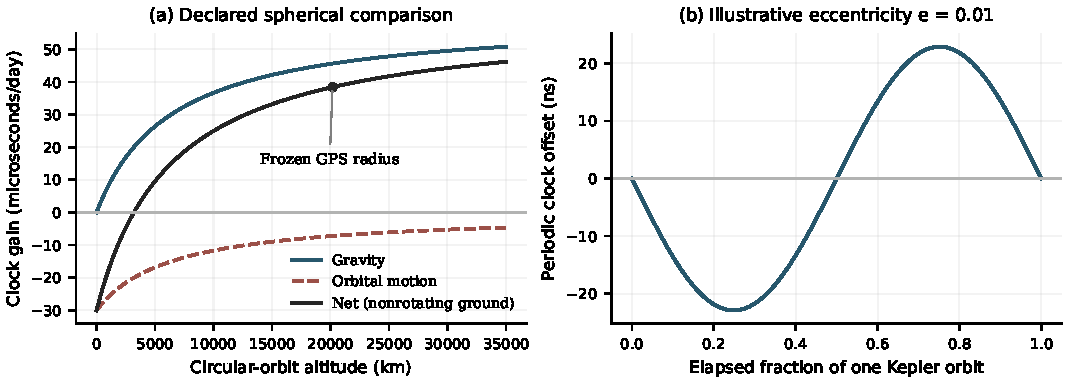
\includegraphics[width=\textwidth]{orbital_clock_controls.pdf}
\caption{Declared orbital controls, not fitted GPS data. (a) The first-order monopole gravitational, kinetic and net rates relative to a nonrotating spherical ground reference. The marked radius uses the frozen GPS arithmetic operands; the zero crossing follows from the same circular-orbit law. (b) The eccentricity clock offset for a declared Kepler orbit with $e=0.01$, plotted against elapsed orbital fraction from perigee. Its amplitude is $22.8966$ ns and its mean is zero; an interval comparison uses the difference of its endpoint values. Ground-reference rotation, actual geopotential harmonics, clock steering and propagation are separate inputs.}
\label{fig:orbitcontrols}
\end{figure*}


\section{Optical height and endpoint uncertainty}\label{app:height}


\subsection{A local height comparison is a separate channel}
GPS combines a gravitational potential difference, orbital motion and a reference time scale. A pair of nearly stationary clocks separated vertically supplies a different test. Let $h$ be upward height from a lower radius $r$, and initially use the spherical source. Rationalizing the exact endpoint ratio gives
\[
\begin{aligned}
 q_h&=\sqrt{\frac{1-a(r+h)}{1-a(r)}}-1,\\
 &=\frac{a(r)-a(r+h)}{(1-a(r))\left[\sqrt{\frac{1-a(r+h)}{1-a(r)}}+1\right]}.
\end{aligned}
\]
This expression is numerically stable at laboratory heights. Since
\[
 a(r)-a(r+h)=\frac{2\mu h}{c^2r(r+h)},\qquad \mu=GM,
\]
its leading value is $gh/c^2$, with $g=\mu/r^2$. In a real laboratory, the corresponding quantity is the local geopotential difference, including the reference's rotational contribution. A height alone is an approximation to that potential difference.

Bothwell and colleagues resolved a spatial clock-frequency gradient across a millimetre-scale strontium sample. Their corrected result is $-9.8(2.3)\times 10^{-20}\,\mathrm{mm}^{-1}$ in their coordinate convention, compared with the expected approximately $-10.9\times 10^{-20}\,\mathrm{mm}^{-1}$. Density, magnetic-field and other gradient systematics are included in the published analysis. The separately reported $7.6\times 10^{-21}$ synchronous comparison uncertainty is not the uncertainty of this gravitational gradient.~[8]

The recovered SAM CR006 packet uses the upward-positive convention, $g=9.796\,\mathrm{m\,s^{-2}}$, and a one-millimetre separation. It obtains approximately $1.0899520\times 10^{-19}$ and a residual of $0.478$ quoted standard deviations from the positive measured gradient.~[7] Its effective radius is chosen as $\sqrt{\mu/g}$, so the leading prediction already imports the local acceleration. The result is a useful consistency check on the endpoint coefficient and sign; it does not establish the inverse-radius profile independently across one millimetre, and it does not distinguish SAM from general relativity when their predictions agree.


\label{app:errors}


\subsection{A comparison must carry its error budget}
The difference between two endpoint rates is not automatically the ratio of two received signals. A transmitted comparison contains range-rate Doppler, propagation, synchronization and hardware contributions. Controlled transport introduces a trajectory and acceleration history. A useful test must state how those terms are removed or modeled before a residual is assigned to the endpoint law. It must identify which corrections and steering have already been applied to each timestamp, and retain the initial epoch and full observation interval. A short orbital segment can confuse a constant bias with part of a periodic residual. Rotating-frame propagation corrections remain necessary when that frame is used; the geoid rotation term in the clock rate does not replace them.~[4,5,10]

A simple bound makes the metrological requirement explicit. Within the declared first-order rate model, suppose $|\delta\Phi|\le\epsilon_\Phi$, $|\delta\Phi_0|\le\epsilon_0$ and $\|\delta\mathbf v\|\le\epsilon_v$. Then
\[
 |\delta q|\le
 \frac{\epsilon_\Phi+\epsilon_0+|\mathbf v|\epsilon_v+\epsilon_v^2/2}{c^2}.
\]
\textit{Proof.} Expand $|\mathbf v+\delta\mathbf v|^2-|\mathbf v|^2=2\mathbf v\cdot\delta\mathbf v+|\delta\mathbf v|^2$ and apply Cauchy--Schwarz. For equal initial clock offsets, integration gives $|\delta\tau|\le\int|\delta q|\,dt$, or $T\sup|\delta q|$ over a duration $T$. Two independently uncertain endpoints require both budgets. This is a bound on parameter errors in the stated rate law, not a complete receiver uncertainty analysis.

Near the surface, a one-metre geopotential-height error corresponds to about $1.09\times 10^{-16}$ fractional rate and $9.42$ picoseconds accumulated per day for the declared local $g$. A centimetre therefore matters near the $10^{-18}$ scale. These conversions are sensitivity estimates; they do not assign an uncertainty to a particular apparatus.

Pure relativistic truncation can be bounded separately. For $0\le x\le b<1$, Taylor's theorem gives
\[
 0\le 1-\frac{x}{2}-\sqrt{1-x}
 \le\frac{x^2}{8(1-b)^{3/2}}.
\]
The second derivative of $\sqrt{1-x}$ is $-1/[4(1-x)^{3/2}]$, which proves the bound. The exact remainder is
\[
 \sqrt{1-x}-1+x/2=-\frac{x^2}{2(1+\sqrt{1-x})^2}.
\]
Small omitted powers of a declared metric are not bounds on missing quadrupole fields, tides, ephemeris errors, clock steering, temperature shifts or the as-yet-uncontrolled nonuniform source coupling. Those require their own inputs and estimates.


\section{Solar timing operands and approximation certificates}\label{app:solar}


\subsection{The retained solar geometry}
The recovered solar CR006 packet declares $G=6.6743\times 10^{-11}$ SI, $M_\odot=1.98847\times 10^{30}$ kg, $c=299792458\,\mathrm{m\,s^{-1}}$, $R_\odot=695700000$ m and $1\,\mathrm{AU}=149597870700$ m. It places endpoints at radii $r_A=1$ AU and $r_B=8.43$ AU, on opposite sides of a closest approach $b=1.6R_\odot$. The resulting source length and straight-segment length are approximately
\[
 r_s=2953.3393821\ {\rm m},\qquad
 L=1.41070328817\times 10^{12}\ {\rm m}.
\]
At $\gamma=1$ its archived witnesses are
\[
 \int a\,\dd\ell=39337.4321183\ {\rm m},\qquad
 \Delta T_1=131.215549520\ \mu{\rm s}.
\]
The ideal frozen symmetric two-way value is twice the one-way value. None of these is a direct measurement of a Cassini tracking pass.~[15]

The retained photon-draft companion calculation compares the $\operatorname{asinh}$ primitive, the finite-endpoint logarithm and numerical quadrature. Their agreement checks one mathematical integral through different implementations. It does not create three independent observations. The archive uses $GM_\odot=1.3271645321\times 10^{20}\,\mathrm{m^3\,s^{-2}}$ from its separately frozen $G$ and mass. Substituting the different reference operand $1.32712440018\times 10^{20}$ gives about $131.211581713$ microseconds in the same geometry. That input change is not a relativistic correction or a newly inferred value of $\gamma$.

\begin{table}[htbp]
\centering\small
\caption{Retained opposite-side impact sweep, holding endpoint radii fixed. Rounded arithmetic values, not observed tracking data.}
\begin{tabular}{@{}rrr@{}}\toprule
$b/R_\odot$ & $1/r$ road ($\mu$s) & Normalized $1/r^2$ ($\mu$s)\\\midrule
1.2 & 136.883683 &175.070258\\
1.6 & 131.215550 &131.215550\\
3.0 & 118.830002 &69.818952\\
10.0 &95.103737 &20.701578\\\bottomrule
\end{tabular}
\end{table}
The inverse-square control is normalized to the central case. Its other cases then expose a different shape. Half and double source amplitude give half and double delay; the missing-road control gives zero by definition. These are useful operator checks, but the latter does not rule out every conceivable endpoint-based theory. The archive's $\gamma_{\rm eff}=1$ follows from its imposed road coefficient, rather than a fit to raw Cassini observations. Its broad central-delay interval and simplified gamma gate must be read in that limited role.~[15]


\subsection{Which approximation is being bounded?}
A numerical residual is useful only when its target is named. Three differences already occur in the frozen solar example. First, the finite logarithm differs from its far-endpoint approximation by about $138.275$ picoseconds. Second, changing the imported solar $GM$ changes the one-way prediction by about $3.968$ nanoseconds. Third, choosing higher-order metric coefficients would change the optical index and the ray. These are distinct effects with different physical meanings.

A controlled index example illustrates the distinction. Deliberately treat the truncated expressions $N^2=1-a$ and $h_{ij}=(1+a)\delta_{ij}$ as exact functions. Their index is
\[
 n_{\rm opt,*} =\sqrt{\frac{1+a}{1-a}}.
\]
This defines a comparison model; the original first-order metric did not specify these higher-order coefficients. For $0\leq a\leq\epsilon<1$, algebra gives
\[
 n_{\rm opt,*}-(1+a)=\frac{a^2(1+a)}{(1-a)(n_{\rm opt,*}+1+a)}\geq 0.
\]
Since the denominator's last factor is at least two,
\[
 0\leq\delta T_{\rm index}
 \leq\frac{1+\epsilon}{2c(1-\epsilon)}\int_{\Gamma_0}a^2\,\dd\ell.
\]
For the monopole straight segment,
\[
 \int a^2\,\dd\ell
 =\frac{r_s^2}{b}
  \left[\arctan(z_B/b)-\arctan(z_A/b)\right].
\]
In the frozen CR006 geometry, direct quadrature gives about $40.9480$ picoseconds for this stipulated fixed-path index remainder, below its $40.9482$ picosecond bound. This is a stringent check of that mathematical remainder, not an uncertainty bound on the physical Shapiro prediction. It excludes ray bending, unspecified metric terms, source motion, multipoles, plasma and apparatus. An exact Schwarzschild metric would have its own higher-order lapse and spatial coefficients; it is not obtained by declaring this truncation exact.

A complete accuracy claim therefore needs a hierarchy: source-input errors, metric-order remainder, path perturbation, dynamical geometry, transfer medium and measurement reduction. Small disagreement between two formulas for the same first-order integral controls implementation, not that entire hierarchy.


\subsection{The local background and the cosmological road}
The local solar calculation is a source-excess comparison with a declared background route. In the retained linear account, $A_{\rm tot}=A_0+a$ and
\[
 \Delta T_{\rm source}
 =\frac 1c\int_{\Gamma_0}(A_{\rm tot}-A_0)\,\dd\ell
 =\frac 1c\int_{\Gamma_0}a\,\dd\ell.
\]
The subtraction uses the same route and reference convention. It does not delete the background from the theory. More generally an optical comparison subtracts the chosen reference index: $c^{-1}\int(n_{\rm opt}-n_{\rm opt,ref})\,\dd\ell$, with endpoint units and geometry calibrated consistently.

The archive's deliberately un-subtracted floor control adds $A_0L/c$ with $A_0=1/(12\pi)$. It produces approximately $124.820038876$ seconds including the small source term, rather than the $131.216$ microsecond source excess.~[15] That result demonstrates the consequence of inserting a uniform baseline into this already source-subtracted observable. It is not a measurement excluding every homogeneous background, since a homogeneous index also changes coordinate and calibration conventions.

This linear road subtraction differs from the nonlinear raw-lapse normalization discussed above. A constant inside $\sqrt{1-A_0-a}$ changes the source coefficient after normalization; it cannot be removed by claiming that every local operation subtracts the floor. The receiving law must be stated before the background operation is performed.~[3,11]

The redshift-indexed amplitude-distance construction has its own source, propagation, detector and calibration inputs. Its finite-window inference is developed in the main text; it is not inserted into this source-excess timing integral. The Magic Bell remains a conceptual prompt rather than a global horizon theorem.

\section{Quantum-form and source-matrix certificates}\label{app:form-proof}
\subsection{Closedness and complete counterterm}
The graph norm $\|\Psi\|^2+\|T_g\Psi\|^2$ is equivalent to the free-field form norm by Eq.~\eqref{eq:equivalent-forms}. A weight $W$ bounded above and strictly below multiplies this squared map norm by equivalent constants. Completeness therefore proves closedness on the unchanged $Q(H_f)$; bounded source terms preserve closedness and a finite lower bound. Expansion of the same square supplies all free, interaction and counterterm pieces on that one domain. This argument uses $\int|u|^2/\omega<\infty$ and does not require $\int|u|^2<\infty$.

A finite exact source certificate makes the weighted counterterm concrete. On the two original polarizations choose
\[
 W=\begin{pmatrix}1&\ii/4\\-\ii/4&1\end{pmatrix},\qquad
 \operatorname{spec}W=\{3/4,5/4\}.
\]
Using the actual sixteen-state source and $C=\ii SD$, the counterterm divided by $\varepsilon^2\mu$ is
\[
 B_{\rm ct}=D^2+C^2+\frac{\ii}4(DC-CD)
 =2D^2+\frac 12SD^2.
\]
With $P_\pm=(I\pm S)/2$, the exact Gram factorizations are
\[
 B_{\rm ct}-\tfrac 32D^2=(DP_+)^*(DP_+),\qquad
 \tfrac 52D^2-B_{\rm ct}=(DP_-)^*(DP_-).
\]
Both $B_{\rm ct}$ and $D^2$ have rank twelve; each comparison has rank six. The four dark source dimensions are retained. This order-one polarization weight is an algebra certificate, separate from the small-$\delta$ phase-sign fixture in Table~\ref{tab:form-budgets}.

\subsection{Bootstrap energy inequality}
Remove the same even scalar from both static generators for the state comparison, while retaining it in their original energies. Conservation of the actual energy gives
\[
 N\varepsilon\langle S\rangle_{\rm act}+NK_{\rm act}+r[\Psi,\Psi]
 =N\varepsilon\langle S\rangle_0+NK_0+r[\Psi_0,\Psi_0].
\]
Subtract the corresponding conserved reference energy. The source expectation difference is at most $2d_\Psi$ because $\|S\|=1$; the form errors are bounded by $\delta K_{\rm act}$ and $\delta K_0$. Using $K_0,K_{\rm ref}\le\kappa$ gives the inequality in the main text. Together with the weak overlap identity it proves the stated first-crossing bound, without resolving unbounded field energy into separate poorly conditioned marginals.

\subsection{Common-form first-order current response}
For $q_\lambda=q_0+\lambda r_B$, equivalent form norms supply a common finite-energy space and uniform bounds for sufficiently small $\lambda$. Form-resolvent convergence gives strong Hilbert-space convergence of the evolved fixed preparation; the common energy bound gives weak form-space convergence. Conservation of $q_\lambda$ and the continuous bounded source term give convergence of the shifted $q_0$ norm. Weak convergence plus norm convergence is strong convergence in that form Hilbert space.

The exact weak variation identity can consequently be divided by $\lambda$ and passed to zero in its continuous pairings under a common integrable bound. This gives the displayed $z_1$ formula. A finite-energy preparation derivative adds its separate initial-state response. A uniform variation of every complete Hamiltonian term reduces to the exact internal-age derivative. A nonconstant output weight supplies a different, explicitly incidence-dependent response functional.

\section{Statistical and reconstruction certificates}\label{app:statistics}
\subsection{Contrast equals generalized least squares}
At a trial exponent $p$, let $t_i=e^{-ps_i}$ and $X_p=[\bm 1,\bm t]$. Form the consecutive contrast matrix $A_p$ with row entries $[\lambda_i,-(1+\lambda_i),1]$, where
\[
 \lambda_i=\frac{t_{i+2}-t_{i+1}}{t_{i+1}-t_i}.
\]
Each row annihilates both columns of $X_p$. For distinct ordered samples and $p>0$, the $m-2$ rows are linearly independent: the last nonzero column of each successive row gives a triangular independence argument. Thus their row space is the full annihilator of the two-column model.

Let $\Sigma=LL^T$ be positive definite, $\bm z=L^{-1}\bm y$, $Z=L^{-1}X_p$ and $B=A_pL$. Since $BZ=0$ and both spaces have the complementary dimensions,
\[
 B^T(BB^T)^{-1}B=I-Z(Z^TZ)^{-1}Z^T.
\]
Sandwiching between $\bm z^T$ and $\bm z$ gives
\[
 (A_p\bm y)^T(A_p\Sigma A_p^T)^{-1}A_p\bm y
 =(\bm y-X_p\widehat{\bm\vartheta})^T\Sigma^{-1}
 (\bm y-X_p\widehat{\bm\vartheta}).
\]
The projector has rank $m-2$. For fixed $p$, known covariance and a Gaussian model, this proves the stated $\chi^2_{m-2}$ law. Profiling $p$ changes the procedure and its calibration.

\subsection{Constant-ratio search and exponent profiling}
Whiten the data, project out the constant direction, and normalize the remaining $\bm t_p$ direction to $\bm q_p$. On a finite predeclared grid $\mathcal G$, the improvement over a constant fit is
\[
 \Delta_{\mathcal G}=\max_{p\in\mathcal G}(\bm q_p^T\bm z)^2.
\]
Under the constant-ratio null these form a correlated unit-variance Gaussian process on the same grid. Standard-normal simulations through that grid calibrate the complete search. The constant-ratio result concerns measured evolution; the separate single-power residual concerns the adequacy of its shape. Neither uses a one-exponent threshold after a grid search.~[19]

\subsection{Noisy Hankel determinant}
For increments $\bm d=\bm\mu+\bm e$ with covariance $V$, take $B_{02}=B_{20}=1/2$, $B_{11}=-1$ and all other entries zero. Then
\[
 E[\bm d^TB\bm d]=\bm\mu^TB\bm\mu+\Tr(BV).
\]
The bias-corrected determinant and its Gaussian variance are
\[
 \widehat H_c=d_0d_2-d_1^2-V_{02}+V_{11},
\]
\[
 \Var(\widehat H_c)=2\Tr(BVBV)+4\bm\mu^TBVB\bm\mu.
\]
The variance follows by expanding the quadratic form and applying the Gaussian second/fourth moments. Bias correction does not turn a quadratic statistic into a Gaussian one; calibrate its tails under the declared mean and covariance model.~[19]

\subsection{Calibration, Fieller set and information}
For fixed $p$, let $V=\Cov(\widehat\alpha,\widehat\beta)$ and $\widehat C_{\rm cal}=\widehat\alpha+\widehat\beta$. The coefficient variances are
\[
 v_{\alpha\alpha}=V_{00},\quad
 v_{CC}=V_{00}+2V_{01}+V_{11},\quad
 v_{\alpha C}=V_{00}+V_{01}.
\]
Inverting the Gaussian test for the linear combination $\alpha-xC_{\rm cal}$ gives the fixed-exponent Fieller set
\[
 (\widehat\alpha-x\widehat C_{\rm cal})^2
 \le k_\rho^2(v_{\alpha\alpha}-2xv_{\alpha C}+x^2v_{CC}).
\]
It may be bounded, disconnected or unbounded according to normalization information. For independent weights $w_i$, direct evaluation of the two-by-two coefficient matrix gives
\[
 \det(X_p^TWX_p)=\left(\sum_iw_i\right)^2\Var_w(t_i).
\]
This is the exact leverage certificate: nearly equal $t_i$ make the constant and transient columns difficult to separate.

If a covariance mode is $\Sigma_{\rm sys}=X_p\Omega X_p^T$, then $A_p\Sigma_{\rm sys}A_p^T=0$. Such a mode changes coefficient uncertainty without adding shape residual. A general redshift-dependent calibration template has a component outside that space.

\subsection{Held-out prediction with cross-covariance}
Partition the observations into training $T$ and held-out $H$. At fixed $p$, define
\[
 K=\Sigma_{HT}\Sigma_{TT}^{-1},\quad
 V_T=(X_T^T\Sigma_{TT}^{-1}X_T)^{-1},\quad
 B_H=X_H-KX_T.
\]
The training-only predictor and error covariance are
\[
 \widehat{\bm y}_H=K\bm y_T+B_H\widehat{\bm\vartheta}_T,
\]
\[
 V_H=\Sigma_{HH}-K\Sigma_{TH}+B_HV_TB_H^T.
\]
To prove the covariance, write $\bm y_H=K\bm y_T+B_H\bm\vartheta+\bm\epsilon_c$, where Gaussian conditioning makes $\bm\epsilon_c$ independent of the training data with covariance $\Sigma_{HH}-K\Sigma_{TH}$. Subtract the predictor and add the independent coefficient-estimation term. The $V_H$-weighted squared error is $\chi^2_{|H|}$ under the fixed-exponent Gaussian model. If training selects $p$, that selection is repeated in its calibration.~[19]

\subsection{Bin windows and ratio covariance}
For normalized bin windows $W_i(s)$, replace $t_i=e^{-ps_i}$ by
\[
 t_i(p)=\int W_i(s)e^{-ps}\,\dd s.
\]
A Gaussian window of variance $v_i$ gives $t_i=e^{-ps_i+p^2v_i/2}$; a top-hat window of half-width $h_i$ gives $t_i=e^{-ps_i}\sinh(ph_i)/(ph_i)$. Unequal widths can create a deterministic shape residual when only bin centers are used.

For jointly estimated positive channel distances $G_i,E_i$ and $Y_i=G_i/E_i$, the leading ratio Jacobian is
\[
 J_Y=\left[\diag(E_i^{-1}),-\diag(G_i/E_i^2)\right],\qquad
 \Sigma_Y\simeq J_YV_{GE}J_Y^T.
\]
Keep the cross-channel and cross-redshift blocks. Broad or non-Gaussian likelihoods use joint positive-distance likelihood/posterior samples in place of the linear expansion. A detected-event population also has selection normalization
\[
 \mathcal A(\vartheta)=\int p({\rm detected}\mid\theta,\vartheta)
 \pi(\theta\mid\vartheta)\,\dd\theta.
\]
An amplitude-law change can alter this normalization; widening ratio error bars does not encode that change.~[19]

\section{Finite-window endpoint proofs}\label{app:minimax}
\subsection{Correlated Gaussian two-point bound}
For two mean curves with finite sample-vector difference $\bm\Delta$ and common positive-definite covariance $\Sigma$,
\[
 D_{\rm KL}=\tfrac 12\bm\Delta^T\Sigma^{-1}\bm\Delta
 \le\frac{m\|\bm\Delta\|_\infty^2}{2\lambda_{\min}(\Sigma)}.
\]
For the slow-mode construction in the text, $\|\bm\Delta\|_\infty\le B\epsilon s_{\max}$. Choosing
\[
 \epsilon\le\frac{\sqrt{\lambda_{\min}(\Sigma)}}{B s_{\max}\sqrt m}
\]
makes $D_{\rm KL}\le 1/2$. Pinsker's inequality gives total variation at most $1/2$. To turn an estimator into a test, assign it to the nearer of the two plateau values. An erroneous assignment entails endpoint estimation error at least $B/2$; the sum of test-error probabilities is at least $1-\mathrm{TV}$. Hence every estimator obeys
\[
\begin{aligned}
 \max_jP_j(|\widehat \Xi_\infty-\Xi_{\infty,j}|\ge B/2)&\ge 1/4,\\
 \max_jE_j|\widehat \Xi_\infty-\Xi_{\infty,j}|&\ge B/8.
\end{aligned}
\]
For the fast-mode pair, replace $B\epsilon s_{\max}$ by $|D|e^{-Ps_{\min}}$ and $B$ by $|D|$. The same argument bounds calibration recovery. These claims concern the stated broad response class; an independently derived rate restriction changes that class.~[19]

\subsection{Positive-spectrum endpoint inequalities}
For a decreasing normalized curve
\[
 \Xi(s)=\Xi_\infty+\int_{p_{\min}}^\infty e^{-ps}\,\dd B(p),\quad
 \dd B\ge 0,\quad\int\dd B=1-\Xi_\infty,
\]
positivity gives $\Xi_\infty\le \Xi(s)$, while $e^{-ps}\le E=e^{-p_{\min}s}$ gives $\Xi(s)\le \Xi_\infty+E(1-\Xi_\infty)$. Rearrangement proves $(\Xi-E)/(1-E)\le \Xi_\infty\le\Xi$. The increasing case follows by applying the same argument to the positive deficit $\Xi_\infty-\Xi(s)$.

At the low endpoint, if $Y_\infty$ is fixed independently and $0<p\le p_{\max}$, then $Y(s)-Y_\infty\ge e^{-p_{\max}s}[C_{\rm cal}-Y_\infty]$ on a decreasing branch. Rearrangement gives the stated upper bound on $C_{\rm cal}$; positivity gives its lower bound. Simultaneous error bands preserve their declared joint coverage under monotone endpoint maps and interval intersection.

\section{Retained synthetic benchmark specification}\label{app:benchmark}
The following numbers are transcribed from the supplied Rev 6 source, not newly generated simulation outputs. Its 24 compressed samples span $z=0.03$ to $2$ equally in $s$, with $(\Xi_\infty,p,C_{\rm cal})=(0.90,3,1.04)$. The marginal fractional scale is $f_i=\sqrt{0.02^2+(0.0225z_i)^2}$, rising from $2.00\%$ to $4.92\%$. An independent centered lognormal component has shape $0.75$ and rms fraction $0.004+0.004z_i$; the remaining Gaussian core has an $80\%$ diagonal and $20\%$ exponentially correlated component in $s$. This is a synthetic compressed-data model, not a survey catalog.

The departures are $Y_{\rm two}/1.04=0.90+0.07e^{-3s}+0.03e^{-s/2}$, $Y_{\rm drift}/1.04=e^{0.01s}(0.90+0.10e^{-3s})$, and a localized feature centered at $s=0.60$, width $0.09$, amplitude $0.015$. The exponent grid is $0.25\le p\le 8$ with step $0.025$. Thresholds use 30000 null catalogs and each reported case 20000 independent test catalogs.~[19]

\begin{table}[htbp]\centering\small
\caption{Rev 6 reported rejection percentages at its percent-level error scale. Both test columns use the reported simulated 5\% threshold.}
\begin{tabular}{@{}lrr@{}}\toprule
Input & Fixed $p=3$ & Profiled $p$\\\midrule
Single power, $C_{\rm cal}=1.04$ &5.09&5.06\\
Same shape, $C_{\rm cal}=0.96$ &4.97&5.15\\
Second power &5.20&5.20\\
Calibration drift &4.97&5.03\\
Localized departure &6.20&5.87\\\bottomrule
\end{tabular}\end{table}
The noiseless fitted $(p,\Xi_\infty)$ are $(2.57760,0.91611)$ for the second power, $(3.34482,0.90972)$ for drift and $(2.95009,0.90775)$ for the localized departure. Their profiled Gaussian-core noncentralities at unit error scale are $0.001343$, $0.002851$ and $0.593907$; fixed-$p$ values are $0.03191$, $0.02624$ and $0.59429$. Under $\Sigma\mapsto c^2\Sigma$, they become $\lambda/c^2$. The reported complete-noise precision sweep uses 40000 independent null checks and 20000 catalogs per departure/precision point. Smooth departures remain close to null rejection after exponent profiling at the $0.3\%$ maximum-error endpoint, while fixed $p=3$ gives approximately $30\%$ and $24\%$ rejection for the second-power and drift examples.~[19]

Other reported internal checks include $95.017\%$ fixed-exponent Fieller coverage from 100000 catalogs, interval $[0.85863,0.94365]$ on the fiducial mean, and inferred calibration standard deviation $0.01595$. The constant-ratio scan threshold is $4.81599$; a separate 20000-catalog sample rejects $5.08\%$, compared with $8.93\%$ when a one-exponent threshold is incorrectly reused. The 16-training/eight-held-out test has mean statistic $8.00894$ and $5.005\%$ rejection over 100000 catalogs. Two overlapping Hankel contrasts have analytic correlation $-0.20587$ and reported simulation correlation $-0.20501$ from 200000 samples. These check separate pieces of one synthetic framework.

With 24 independent ratios of common absolute error $0.03$, the reported local Fisher $(\sigma_p,\sigma_{\Xi_\infty})$ are $(10.8103,0.20500)$ for low-only sampling, $(2.0498,0.02174)$ for broad sampling, $(21.8409,1.20322)$ for high-only sampling and $(1.9063,0.01883)$ for three bands. Low, transition and high-redshift coverage supply different leverage. A top-hat bin example fitted at point centers gives $(p,\Xi_\infty,C_{\rm cal})=(3.01539,0.900323,1.040059)$; the window-aware fixed-$p$ fit recovers the declared fiducial coefficients to its floating-point precision.~[19]

\section{Event-map robustness certificate}\label{app:event-error}
Suppose $F'\ge m_F>0$, $\|\widetilde F-F\|_\infty\le\epsilon_F$, and both inverse branches are defined on the common receiving interval. Monotonicity and the mean-value bound for $F$ give
\[
 |\widetilde F^{-1}(t)-F^{-1}(t)|\le\epsilon_F/m_F.
\]
If $|\theta_E'|\le L_\theta$, the encoded phase uncertainty is therefore at most $L_\theta\epsilon_F/m_F$. If derivative error at the compared emission events is at most $\epsilon_v<m_F$, then
\[
\begin{aligned}
 \left|\frac 1{\widetilde F'}-\frac 1{F'}\right|
 &\le\frac{\epsilon_v}{m_F(m_F-\epsilon_v)},\\
 |\ln\widetilde F'-\ln F'|&\le-\ln(1-\epsilon_v/m_F).
\end{aligned}
\]
Shifts of the emission argument require a bound on rate variation in addition to this derivative-error budget. With ideal current amplitude $|z|\ge r>0$ and complex error $|\Delta z|\le e<r$, the phase-error disk gives $|\Delta\theta|\le\arcsin(e/r)$ on the continuous branch. Add encoding, transfer-phase, timing, model and readout errors on that branch. Sampling increments and total uncertainty must retain a strict margin below $\pi$, or an independently recorded winding is needed. These bounds supply a ledger interface; their numerical operands come from the apparatus and the actual propagation problem.

\section{Reproduction routes and custody}\label{app:reproduce}
The compact replay packet contains the assembled editable chapter, inherited TeX inserts and figures, new response, canonical, continuum and work/flux derivations, frozen source operands, independent checks and results. It avoids duplicating historical IV/V reconstruction archives. The unchanged predecessor's compact replay was independently rerun here: all eleven steps and fourteen result files matched exactly, with 920 standard-library assertions. That validates its retained execution, while the present directional-kernel and inverse repairs have their own checks.

Run \texttt{python3 ops/reproduce.py} for portable mathematical checks on a disposable relocated copy. Add an explicitly supplied companion evidence ZIP to authenticate all 17 successful native mathematical requests and four local retrievals, using 2,939 assertions and 290 matrix entries. All 126 retained helper files were authenticated and the relocated native readback is byte-identical. The actual run used six controllers, three helpers and two original 180-second admission windows on its own reserved cores; no global startup lease or third round was used. Final completion and release receipts are retained. No replay starts the native engine. Numerical Bessel quadrature is an optional separately labeled diagnostic.

The finite-redshift PDF's embedded artifact link resolves to \url{https://doi.org/10.5281/zenodo.22985359}; its printed text truncates that link. The recovered archive inside the unchanged predecessor source archive identifies itself as a new independent reconstruction of an earlier identifiability manuscript. Its \texttt{PROVENANCE.md} distinguishes preserved paper numbers from new code/results, records unresolved historical covariance and draw-order details, and does not claim recovery of original historical simulation outputs. That archive is retained as a reconstruction, while the supplied Rev 6 PDF remains the authority for the historical benchmark transcribed in Appendix~\ref{app:benchmark}.

The archived GPS, optical and solar packets are arithmetic and scoped external-contact records. No new raw GPS reduction, optical-clock experiment or Cassini tracking fit is claimed by including them. The retained binary-pulsar receipt imports its masses and geometry and is not used as an independent arrival-time fit. The cited G11555 reference index did not supply its original strong-field theorem package; it is retained as a retrieval lead rather than substituted for that result.~[17]

\section{The complete actual-state tail coefficient}\label{app:tail-coefficient}
This explicit coefficient makes the preceding spatial tail bound
independently reproducible. Put $h=64/63$, $c_1=1/4+64/3969$,
$\lambda_\pm=64\Delta_\pm$, $k_0=1/R_-$,
and $(d_1,d_2,d_3)=(1,3,3)$. For $n=0,1,2$, define
\[
 \begin{gathered}
 I_0=(k_0^2-\lambda_-^2)/2,\quad I_1=k_0-\lambda_-,\\
 I_2=(k_0-\lambda_-)/\lambda_-,\quad
 J_n=\frac{k_0^{4-n}-\lambda_-^{4-n}}{4-n},\\
 A_n=\frac{hR_+^2}{15}(\lambda_+^{2-n}+k_0^{2-n})\\
 \hphantom{A_n=}+\frac{R_+^2}{15}[(n+2)h+c_1]I_n
       +\frac{hR_+^4}{105}J_n.
 \end{gathered}
\]
Here $I_2$ is an upper bound for the logarithmic integral, chosen to keep
the executable certificate rational. Then
\[
 \begin{aligned}
 C_A(L)=|g|_+\Bigg\{&\frac34\sum_{p=1}^3d_pL^{1-p}A_{p-1}\\
 &+\frac32\sum_{p,q=1}^3d_pd_qL^{1-p}R_-^{-q}
       k_0^{-(p+q-1)}\\
 &\hspace{3em}\times\left[2h+\frac{c_1}{p+q-1}\right]\Bigg\}.
 \end{aligned}
\]
It is valid for $L\ge2R_+$ and $\lambda_+<k_0$ and retains all nine
large-frequency Bessel products. The conservative constants use
$\pi\ge3$ and $\sqrt\kappa\ge8/9$. The fixed-shift tail adds
$4C_F^2/(5L^5)$ to $8C_A(L)^2/L$, where
\[
 C_F(L)=\frac{16|g|_+R_+^2}
 {15\pi_-\sqrt{\kappa}_-\,(1-y_L^2)},\qquad
 y_L=\frac{2LR_+}{L^2+R_+^2}.
\]
Take $\pi_-=3$ and $\sqrt{\kappa}_-=8/9$ as explicit rational lower bounds. The retained outward source endpoints are used throughout. This is the
original fixed-shift envelope, including its $L$ dependence.
The time-dependent soft comparison and the preparation-energy minimum
are paid separately in $\eta_{\rm ref}(L)$; they are not removed by taking
$L$ large. The compact replay keeps their original source enclosures.

\clearpage\onecolumn
\par\noindent\textbf{Retained predecessor dependency ledger.} This table records the earlier packet. Current canonical closures, local readout and remaining switched-shell/output operands are stated in Section~\ref{sec:composition6-join} and the preceding new sections.\par
\section*{Dependency ledger: physical claims and remaining inputs}
\label{app:dependency-ledger}
\small
\begin{tabularx}{\linewidth}{@{}>{\raggedright\arraybackslash}p{0.19\linewidth}>{\raggedright\arraybackslash}p{0.16\linewidth}X@{}}\toprule
Object&Status&What it establishes and what it still requires\\\midrule
Original source and six clocks&Source-reported&Signed action, even energy, both polarizations, counterterms, exact hard-branch plus soft-vacuum preparation and finite clock window are retained. The new checks consume their outward certificates; they do not rerun the original spectral campaign.\\[0.5em]
Uniform complete lapse&Derived, conditional&The full interacting history follows one internal-age map. A physical law assigning that lapse to a clock or worldline remains an input.\\[0.5em]
Positive spatial receiver&Derived, selected model&The Bessel/TT incidence is positive and has a common continuum domain. Its equality to canonical local stress is not assumed.\\[0.5em]
Physical profile and units&Declared&One positive Plummer body, one compact-body control and one shared SI fixture fix all operands before comparing lanes. The microscopic ruler/action calibration and gravity assignment are not derived from the source ledger.\\[0.5em]
Six signed responses&Derived enclosures&All six finite form-error budgets fit $0.2$ nrad at $7\times10^{-10}$; total sign is negative for every $0<\alpha\le10^{-3}$. Direct orientation contrasts and exact nulls are bounded. Isolated susceptibility signs remain unresolved.\\[0.5em]
Canonical tensor stress&Derived candidate, open completion&The retained action supplies number, pair, source-shell and complement kernels. A specified switch supplies leading pair energy and its scalar loop. Complete transported boundary bounds and instantaneous frequency-form comparisons are derived. Projective implementability, boundary time regularity, joint remainder, finite energy reference and covariant support law remain open.\\[0.5em]
Gradient return&Derived static result&The bounded Plummer profile has a controlled nonzero static Schur return through magnetic degree2 and electric degree3 sectors. This is not a joint quantum expectation or gradient-sign tomography.\\[0.5em]
Event maps&Derived, conditional&Actual endpoint epochs, proper waits and the moving transfer Jacobian compose correctly under the declared metric and travel approximation. Ephemerides, medium and observational nuisance inputs remain external.\\[0.5em]
Original carrier&Derived, prescribed source&The compact pulse has near, induction and radiation terms, edge-uniform remainders, a 6.25\% peak waveform correction and a signed whole-pulse energy deficit below $6.633\times10^{-14}$, exact positive near storage and complete maintained-source work balance. It remains a maintained four-cycle source protocol, distinct from the autonomous one-cycle clock certificate.\\[0.5em]
Amplitude coefficient&Open physical bridge&Localized source elimination gives its actual retarded kernel and passive spectral weight. It does not yet derive a homogeneous cosmological $Q$ or its background evolution.\\[0.5em]
Positive rate spectrum&Derived Euclidean observable&The actual dressing vector gives a positive continuous, gapless Euclidean measure. Its transform and gap-free slow mass are calculated; exact Hankel rank is infinite. A relaxation law, detector readout and mapping to $\log(1+z)$ are required for a physical distance-rate interpretation.\\[0.5em]
Noisy mode inference&Derived, conditional&One known-covariance event and positive support constraints certify finite-window curve bounds and minimum visible rank. Positive Gaussian quadrature now matches finite continuum samples with signed holdout bounds. Noisy exact mode counts or unrestricted plateau accuracy remain unsupported.\\[0.5em]
Metrology&Specified requirements&Coarse winding and fine final sampling give a sufficient preparation count near $2.173\,10^{22}$. Statistical coverage is conditional on all systematic bounds; no apparatus performance is claimed.\\\bottomrule
\end{tabularx}

\clearpage\twocolumn
\section*{References and source routes}
\begingroup\footnotesize\raggedright
\noindent[1] S. Brady, OpenAI ChatGPT and Codex. \emph{Original Write histories and an interacting source-field action}. Volume I, Chapter I, final source and clock certificates, 15 October 2026. \url{https://github.com/iwtbotiwtwot/sam_volume_I_i}.

\noindent[2] Same authors. \emph{Retention, accumulation, and the finite ledger}. Chapter II source-to-field update, 15 October 2026. \url{https://github.com/iwtbotiwtwot/sam_volume_I_ii}. The retained 24-page/48-section source supplies the physical reference and measurement protocols.

\noindent[3] Same authors. \emph{The spherical accumulation kernel and the source-to-field interface}. Chapter III local-action and quantum-source development, 15 October 2026. Retained 21-page/42-section source and linked certificates.

\noindent[4] N. Ashby. \emph{Relativity in the Global Positioning System}. Living Reviews in Relativity 6, 1 (2003), publisher PDF revision 21 June 2007, equations (12), (16), (18), (21), (27), (35)--(40). \url{https://doi.org/10.12942/lrr-2003-1}.

\noindent[5] GPS Directorate. \emph{IS-GPS-200N: NAVSTAR GPS Space Segment/Navigation User Segment Interfaces}, 1 August 2022, sections 3.3.1.1 and 20.3.3.3.3.1. \url{https://archive.gps.gov/technical/icwg/IS-GPS-200N.pdf}. This chapter retains the version-specific convention supplied with the original endpoint draft.

\noindent[6] SAM Research Project. \emph{CR005: Clocks and GPS external contact}. Courtroom revision \nolinkurl{b5e914f71377e86ef4c67e199973d9300795cda1}. \url{https://github.com/iwtbotiwtwot/The_Courtroom/tree/b5e914f71377e86ef4c67e199973d9300795cda1/03_CLOCKS_AND_GPS/CR005_CLOCKS_AND_GPS_EXTERNAL_CONTACT}.

\noindent[7] SAM Research Project. \emph{CR006: Optical-clock height holdout, endpoint A kernel}. Same Courtroom revision. \url{https://github.com/iwtbotiwtwot/The_Courtroom/tree/b5e914f71377e86ef4c67e199973d9300795cda1/03_CLOCKS_AND_GPS/CR006_OPTICAL_CLOCK_HEIGHT_HOLDOUT_ENDPOINT_A_KERNEL}.

\noindent[8] T. Bothwell et al. \emph{Resolving the gravitational redshift across a millimetre-scale atomic sample}. Nature 602, 420--424 (2022), p. 423 and Extended Data Table 1. \url{https://doi.org/10.1038/s41586-021-04349-7}. NIST publisher-version copy: \url{https://tsapps.nist.gov/publication/get_pdf.cfm?pub_id=933368}.

\noindent[9] S. Brady, OpenAI ChatGPT and Codex. \emph{SAM Unified Technical Synthesis---Volume I}, supplied manuscript, sections 3.1--3.6, Magic Bell printed p. 4, appendices A.5--A.6. Retained endpoint text: \url{https://github.com/iwtbotiwtwot/SAMA/blob/4c2b5dc1649da5900c90b90d0ce56c223dbb7717/vol_i/03-clocks-and-light/endpoint-clock-comparison-and-time-dilation.md}.

\noindent[10] N. Ashby and M. Weiss. \emph{Global Positioning System Receivers and Relativity}. NIST Technical Note 1385 (1999), sections 2.3 and 2.7. \url{https://tf.nist.gov/general/pdf/1274.pdf}.

\noindent[11] S. Brady, OpenAI ChatGPT and Codex. \emph{Endpoint clocks, motion, and the GPS comparison}. Supplied Chapter IV development draft and source/check bundle, 16 October 2026. Preserved unchanged in the predecessor archive, \texttt{inputs/iv/}.

\noindent[12] P. Teyssandier and C. Le Poncin-Lafitte. \emph{General post-Minkowskian expansion of time transfer functions} (2008), arXiv:0803.0277, equations (57), (67). \url{https://arxiv.org/abs/0803.0277}.

\noindent[13] I. I. Shapiro. \emph{Fourth Test of General Relativity}. Physical Review Letters 13, 789--791 (1964). \url{https://doi.org/10.1103/PhysRevLett.13.789}.

\noindent[14] B. Bertotti, L. Iess and P. Tortora. \emph{A test of general relativity using radio links with the Cassini spacecraft}. Nature 425, 374--376 (2003). \url{https://doi.org/10.1038/nature01997}. Also the 2004 Bertotti author presentation linked in the supplied photon draft, with delay-derivative sign conventions distinguished.

\noindent[15] SAM Research Project. \emph{CR006: Photon road Shapiro external contact}. Same pinned Courtroom revision. \url{https://github.com/iwtbotiwtwot/The_Courtroom/tree/b5e914f71377e86ef4c67e199973d9300795cda1/04_PHOTON_ROAD_SHAPIRO_DELAY/CR006_PHOTON_ROAD_SHAPIRO_EXTERNAL_CONTACT}. Distinct from optical-clock CR006.

\noindent[16] A. Hees, S. Bertone, C. Le Poncin-Lafitte and P. Teyssandier. \emph{Range, Doppler and astrometric observables computed from time transfer functions: a survey} (2014), arXiv:1412.3360, equations (2)--(4). \url{https://arxiv.org/abs/1412.3360}.

\noindent[17] SAM Research Project. Retained CR148 binary-pulsar receipt and SAMA G11555 reference index, at the Courtroom revision above and SAMA revision \nolinkurl{4c2b5dc1649da5900c90b90d0ce56c223dbb7717}. Their evidence roles are stated in Appendix~\ref{app:reproduce}; neither supplies a new independent fit or a recovered strong-field theorem here.

\noindent[18] S. Brady, OpenAI ChatGPT and Codex. \emph{Photon roads, the Magic Bell, and Shapiro delay}. Supplied Chapter V development draft and source/check bundle, 16 October 2026. Preserved unchanged in the predecessor archive, \texttt{inputs/v/}.

\noindent[19] S. Brady. \emph{Finite-redshift identifiability of cosmological distance ratios}, Rev 6, supplied 18-page PDF, 26 September 2026. Sections 2--7 and appendices A--B supply the retained amplitude-distance model, finite-window endpoint constructions, reconstruction and statistical benchmark. Embedded artifact link: \url{https://doi.org/10.5281/zenodo.22985359}. Recovered archive provenance is distinguished from original historical results in Appendix~\ref{app:reproduce}.
\noindent[20] NIST Digital Library of Mathematical Functions. Spherical Bessel integral representation, equation 10.54.1. \url{https://dlmf.nist.gov/10.54.E1}. The $n=2$ identity confirms the positive averaging normalization used here.


\noindent[21] A. Balmaseda, D. Lonigro and J. M. P\'erez-Pardo.
\emph{On the Schr\"odinger equation for time-dependent Hamiltonians with
a constant form domain} (2021), Assumption 3.8 and Theorem 3.10.
\url{https://arxiv.org/abs/2112.11063}.

\noindent[22] P. T. Nam, M. Napi\'orkowski and J. P. Solovej.
\emph{Diagonalization of bosonic quadratic Hamiltonians by Bogoliubov
transformations} (2015), Theorem 1, Theorem 2 and the renormalized-operator
remark following them. \url{https://arxiv.org/abs/1508.07321}.


\noindent[23] J. Derezi\'nski. \emph{Bosonic quadratic Hamiltonians}
(2017 revision), Theorems 3.20--3.21.
\url{https://arxiv.org/abs/1608.03289}.
\par\endgroup

\section*{Successor replay and evidence scope}
The new receiving-form, signed-prefix, canonical-coefficient and differential
metrology checks run with \texttt{python3 ops/reproduce.py} from the successor
source packet. Supplying its companion native-evidence ZIP also authenticates
every accepted current native return without starting Duck. Historical replay
counts printed above belong to their unchanged predecessor packets.
The retained joint source manifest authenticates all 193 source members;
the old Downloads ZIP was absent at recovery and has not been reconstructed
or represented as recovered. The complete retained member tree is included.
The final successor verification records current counts, offline PDF build,
all-page visual review and relocated source/native readback.

\section*{Retained C6 replay and evidence scope}
The new static canonical joint, weighted-frame/free-switch, real-time memory,
local-pointer and composed-record checks run with
\texttt{python3 ops/reproduce.py} from the composition source packet.
Its companion native-evidence ZIP authenticates every admitted current
request, complete successful output and retained failure without starting
Duck. Eleven native mathematical requests completed; one exceeded the
installed scalar input-length budget. Its exact bounded replacement is
independently checked but was not admitted after the original deadline.
All four local-corpus retrievals completed. Six controllers and three helpers
used two 180-second windows and own-core locks, with no global startup lease,
third round or automatic repeat.

Historical replay counts and statuses above describe their retained packets.
The actual predecessor source ZIP is now available and included unchanged:
438 manifest-listed files plus its manifest, including the earlier
193-member authenticated source tree. The new replay checks their bytes;
it does not rerun historical research. Final verification records the
current counts, offline PDF build, all-page visual review and relocated
source/native readback.

\section*{Current C7 replay and evidence scope}
The current finite-preparation, paired-cap, complete tensor and joint-domain
proof checks run with \texttt{python3 ops/reproduce.py}. The companion native
evidence packet retains every admitted request, full output, failure and
bounded correction, with source hashes and portable independent readback.
Twelve native requests completed; two original preparation requests failed
because of an extra payload field. Both corrected requests were admitted
inside the original second window and completed. The failures remain
unchanged. Four local-corpus retrievals completed. Six controllers and three
helpers used exactly two 180-second admission windows on their own cores,
with no global startup lease, third round or automatic repeat.

The actual C6 predecessor ZIP is retained unchanged: 264 listed files plus
its manifest. Its embedded C5 source ZIP has 438 listed files plus its
manifest and includes the preceding authenticated 193-file source tree.
The current replay checks those bytes without rerunning historical research.
Historical counts and status statements elsewhere retain their original scope.

\section*{Data and code availability}
The compact source packet contains this editable combined chapter, frozen source operands, derivations, executable checks and results. A separate full native-evidence packet retains the completed execution and custody records. The unchanged predecessor archive retains the original IV/V bundles and historical reconstruction provenance. The chapter source uses $N$ for lapse, $n_{\rm opt}$ for optical index and $p$ for the distance exponent throughout. Original inputs retain their original notation and evidence identities.
\end{document}
